% ============================================================
%  Rapport PFE – 
%  main.tex — fichier principal (inclut les chapitres séparément)
%  Compilé avec pdflatex (2 passes)
% ============================================================

\documentclass[12pt,a4paper]{report}

% ---- Encodage et langue ----
\usepackage[utf8]{inputenc}
\usepackage[T1]{fontenc}
\usepackage[french]{babel}
% ---- Mise en page ----
\usepackage[top=2.5cm, bottom=2.5cm, left=3cm, right=2.5cm]{geometry}
\usepackage{setspace}
\onehalfspacing

% ---- Polices et typographie ----
\usepackage{lmodern}
\usepackage{microtype}

% ---- Graphiques et couleurs ----
\usepackage{graphicx}
\usepackage[table,xcdraw]{xcolor}
\definecolor{primaryblue}{RGB}{31, 73, 125}
\definecolor{lightgray}{RGB}{242, 242, 242}

% ---- Couleurs SAP (chapitre 4) ----
\definecolor{SAPBlue}{RGB}{0, 120, 215}
\definecolor{SAPLightBlue}{RGB}{218, 237, 255}
\definecolor{SAPGreen}{RGB}{50, 168, 82}
\definecolor{SAPLightGreen}{RGB}{220, 245, 228}
\definecolor{SAPOrange}{RGB}{232, 120, 0}
\definecolor{SAPLightOrange}{RGB}{255, 237, 213}
\definecolor{SAPGray}{RGB}{100, 100, 100}
\definecolor{SAPLightGray}{RGB}{245, 245, 245}
\definecolor{SAPRed}{RGB}{200, 50, 50}
\definecolor{CodeBg}{RGB}{248, 248, 248}
\definecolor{CodeBorder}{RGB}{200, 200, 200}

% ---- TikZ (schémas et diagrammes) ----
\usepackage{tikz}
\usetikzlibrary{arrows.meta, positioning, calc,
                shapes.geometric, fit, backgrounds,
                shadows, decorations.pathreplacing, patterns}

% ---- Tableaux ----
\usepackage{booktabs}
\usepackage{float}
\usepackage{tabularx}
\usepackage{multirow}
\usepackage{longtable}
\usepackage{array}
\usepackage{ colortbl, xcolor}

% ---- Listes ----
\usepackage{enumitem}

% ---- Boîtes colorées (tcolorbox) ----
\usepackage[most,breakable]{tcolorbox}

\newtcolorbox{definitionbox}[1]{
  enhanced, breakable,
  colback=SAPLightBlue, colframe=SAPBlue,
  fonttitle=\bfseries\color{white},
  title={#1},
  attach boxed title to top left={yshift=-2mm, xshift=4mm},
  boxed title style={colback=SAPBlue, rounded corners},
  rounded corners, arc=3mm
}

\newtcolorbox{remarquebox}{
  enhanced, breakable,
  colback=SAPLightGreen, colframe=SAPGreen,
  fonttitle=\bfseries\color{white},
  title={Remarque},
  attach boxed title to top left={yshift=-2mm, xshift=4mm},
  boxed title style={colback=SAPGreen, rounded corners},
  rounded corners, arc=3mm
}
% \ptag already defined previously
\newcommand{\opnum}[1]{%
  \tikz[baseline=-0.55ex]{%
    \node[circle, fill=SAPBlue, text=white, font=\small\bfseries,
          minimum size=1.5em, inner sep=0pt]{#1};%
  }%
}
\newcommand{\exarrow}{\;\textcolor{SAPBlue!65}{$\to$}\;}
\usepackage{colortbl}   % \rowcolor, \arrayrulecolor
\newtcolorbox{sourcebox}[1]{
  enhanced, breakable,
  colback=SAPLightOrange, colframe=SAPOrange,
  fonttitle=\bfseries\color{white},
  title={#1},
  attach boxed title to top left={yshift=-2mm, xshift=4mm},
  boxed title style={colback=SAPOrange, rounded corners},
  rounded corners, arc=3mm
}
% ===== TikZ & positioning =====
\usetikzlibrary{
    positioning,
    arrows.meta,
    shadows,
    calc
}
\usetikzlibrary{decorations.pathreplacing, fit, backgrounds}

% ===== Float placement =====
\usepackage{float}

% ===== Colors =====
\usepackage{xcolor}

% ── Packages (if not already present) ──
\usepackage{xcolor}
\usepackage{tikz}
\usepackage{tcolorbox}
\usepackage{booktabs}
\usepackage{colortbl}
\usetikzlibrary{arrows.meta, positioning, fit, backgrounds, shadows}
\tcbuselibrary{skins, breakable, most}

% ── Color definitions ──
\definecolor{offlinecolor}{HTML}{1565C0}
\definecolor{onlinecolor}{HTML}{2E7D32}
\definecolor{offlinebg}{HTML}{E3F2FD}
\definecolor{onlinebg}{HTML}{E8F5E9}
\definecolor{arrowcolor}{HTML}{5C6BC0}
\definecolor{stepbg}{HTML}{EDE7F6}
\definecolor{stepfg}{HTML}{4527A0}
% ===== SAP Color Palette =====
\definecolor{SAPBlue}{HTML}{0A6ED1}
\definecolor{SAPLightBlue}{HTML}{EAF3FC}

\definecolor{SAPGreen}{HTML}{107E3E}
\definecolor{SAPLightGreen}{HTML}{EAF7ED}

\definecolor{SAPOrange}{HTML}{E9730C}
\definecolor{SAPLightOrange}{HTML}{FFF3E8}

\definecolor{SAPGray}{HTML}{5B5B5B}

% ---- Listings (code) ----
\usepackage{listings}
\usepackage{caption}
\usepackage{tcolorbox}
\tcbuselibrary{skins, breakable}
\usepackage{enumitem}
% tikz already assumed loaded

\lstdefinestyle{sapcode}{
  backgroundcolor=\color{CodeBg},
  basicstyle=\ttfamily\small,
  breaklines=true,
  captionpos=b,
  commentstyle=\color{SAPGray}\itshape,
  frame=single,
  framerule=0.5pt,
  rulecolor=\color{CodeBorder},
  keywordstyle=\color{SAPBlue}\bfseries,
  stringstyle=\color{SAPGreen},
  numbers=left,
  numberstyle=\tiny\color{SAPGray},
  numbersep=8pt,
  showstringspaces=false,
  tabsize=2,
  xleftmargin=15pt,
  xrightmargin=5pt,
}
\lstset{style=sapcode}

% ---- En-têtes et pieds de page ----
\usepackage{fancyhdr}
\setlength{\headheight}{14.1pt}
\addtolength{\topmargin}{-2.1pt}
\pagestyle{fancy}
\fancyhf{}
\fancyhead[L]{\small\textit{\leftmark}}
\fancyfoot[C]{\thepage}
\renewcommand{\headrulewidth}{0.4pt}

% ---- Bibliographie ----
\usepackage[numbers,sort&compress]{natbib}

% ---- Hyperliens ----
\usepackage[hidelinks]{hyperref}

% ---- Titres personnalisés ----
\usepackage{titlesec}
\titleformat{\chapter}[display]
  {\normalfont\huge\bfseries\color{primaryblue}}
  {\chaptertitlename\ \thechapter}{20pt}{\Huge}
\titleformat{\section}
  {\normalfont\Large\bfseries\color{primaryblue}}
  {\thesection}{1em}{}
\titleformat{\subsection}
  {\normalfont\large\bfseries\color{SAPGray}}
  {\thesubsection}{1em}{}

% ============================================================
\begin{document}

% ---- Table des matières ----
\tableofcontents
\clearpage

% ---- Chapitres ----

\chapter{Cadre général du projet}
\label{chap:cadre_general}

% ============================================================
\section*{Introduction}
\addcontentsline{toc}{section}{Introduction}

Ce chapitre a pour objectif de présenter le cadre général dans lequel s'inscrit ce projet
de fin d'études. Nous commençons par une présentation de l'organisme d'accueil, puis
nous effectuons une étude de l'existant afin d'identifier les lacunes des solutions actuelles
de surveillance des systèmes SAP. Nous détaillons ensuite la problématique retenue, avant
de présenter la solution proposée et la méthodologie de développement adoptée.

% ============================================================
\section{Présentation de l'organisme d'accueil}
\label{sec:organisme}

\subsection{AVAXIA GROUP}

AVAXIA GROUP est une société de conseil en technologies de l'information à dimension
internationale, fondée en 2006. Elle dispose d'une présence stratégique dans plusieurs
régions, avec son siège social à Dubaï et des centres opérationnels en Tunisie, au Japon
et au Canada. L'organisation est spécialisée dans les solutions technologiques d'entreprise,
avec un accent particulier sur l'implémentation des systèmes ERP (\textit{Enterprise Resource
Planning}), l'intégration de systèmes et les services gérés pour les applications métiers
critiques. Son expertise technique s'étend à l'écosystème SAP ainsi qu'à des plateformes
complémentaires telles que Salesforce.

\begin{figure}[htbp]
  \centering
  
\includegraphics[width=0.35\textwidth]{avaxia_logo.png}

  \caption{Logo Avaxia Group}
  \label{fig:avaxia_logo.png}
\end{figure}

\subsection{Philosophie et approche}

Avaxia Group adopte une méthodologie résolument centrée sur le client dans son modèle
de prestation de services, en privilégiant des partenariats collaboratifs plutôt que des
relations purement transactionnelles.

\subsection{Portefeuille de services}

Avaxia met à disposition  un portefeuille complet de services numériques et de conseil, avec une
forte orientation vers les solutions d'entreprise, le support d'infrastructure et les
technologies émergentes. Le groupe est structuré autour de deux départements spécialisés,
chacun offrant des domaines de services distincts :

\begin{itemize}[leftmargin=*, label=\textbullet]
  \item \textbf{Consultance fonctionnelle :} Conception de solutions métier pour le
        déploiement de nouveaux modules SAP fonctionnels, analyse et optimisation des
        processus de bout en bout, ainsi que la gestion du déploiement fonctionnel et de
        la planification des tests.
  \item \textbf{Big Data :} Services incluant la gestion, la transformation, l'intégration,
        le stockage et l'analyse des données. Les compétences couvrent le développement de
        pipelines de données, les processus ETL et la gouvernance des données.
  \item \textbf{VR / AR :} Développement d'environnements VR interactifs permettant aux
        utilisateurs de naviguer, d'interagir avec des objets et de collaborer en temps
        réel. Les applications comprennent les systèmes de surveillance, les simulations,
        les programmes de formation et les visites virtuelles.
\end{itemize}

\subsection{Structure organisationnelle}

L'architecture organisationnelle d'Avaxia Group est conçue pour faciliter une expertise
spécialisée tout en maintenant une collaboration transversale. La structure du groupe
s'articule autour de trois niveaux :

\begin{itemize}[leftmargin=*, label=\textbullet]
  \item \textbf{Organisation divisionnelle :} Assure les responsabilités de chaque
        département en fonction de son rôle, en gérant le développement commercial et les
        décisions stratégiques.
  \item \textbf{Organisation opérationnelle :} Se concentre sur les défis techniques et
        les expertises qui pilotent les projets et services (planification, exécution,
        livraison et support). Elle permet également de suivre, évaluer et optimiser les
        opérations de projets.
  \item \textbf{Structure corporative :} Supporte le front office en représentant les
        opérations internes (Finance, RH, Formation, Marketing, Qualité de service,
        Informatique), afin d'assurer la continuité de l'activité dans son ensemble.
\end{itemize}

Ce projet se déroule au sein de l'équipe Quadient, rattachée au département
\textit{SAP Infrastructure and BASIS} du bureau tunisien d'Avaxia Group. Les
responsabilités de cette équipe englobent la surveillance et le support des systèmes SAP
critiques auprès de plusieurs clients, ce qui en fait un environnement idéal pour
développer et valider un système avancé de détection d'anomalies basé sur la technologie
RAG.

% ============================================================
% ============================================================
\section{Étude de l'existant}
\label{sec:existant}

Dans le cadre du développement d’un système intelligent de surveillance des systèmes SAP
au sein d’Avaxia Group, une étude de l’existant a été réalisée afin de comprendre les
processus actuels mis en œuvre par l’équipe BASIS.

\subsection*{Rôle du consultant SAP BASIS}

Le consultant SAP BASIS est responsable de l’administration technique des systèmes SAP.
Ses missions principales incluent la surveillance des systèmes, la gestion des performances,
le traitement des incidents techniques ainsi que la maintenance quotidienne des environnements SAP.

Dans le cadre de la surveillance, le consultant BASIS vérifie régulièrement l’état global
du système à travers différentes transactions SAP. Il analyse les jobs en arrière-plan,
les erreurs système, les impressions en attente ainsi que l’activité des processus.
Ces actions permettent d’assurer le bon fonctionnement des systèmes et d’identifier
les anomalies éventuelles.
\subsection*{Surveillance des systèmes SAP}

La surveillance quotidienne des systèmes SAP repose sur l’utilisation de plusieurs codes
de transaction (T-codes), chacun fournissant des informations spécifiques :

\begin{itemize}
    \item \texttt{SM37} : permet de consulter les jobs en arrière-plan et leur état d’exécution.
    \item \texttt{ST22} : permet d’analyser les dumps ABAP générés par les erreurs système.
    \item \texttt{SP01} : permet de visualiser les spools d’impression.
    \item \texttt{DB02} : fournit des informations sur l’état de la base de données.
    \item \texttt{SM66} : permet de superviser les processus actifs du système.
\end{itemize}

Ces transactions sont utilisées de manière régulière par les consultants BASIS afin de
collecter les informations nécessaires à la supervision des systèmes SAP.
% ============================================================
% Schema 1 : Surveillance manuelle des systèmes SAP
% ============================================================
\begin{figure}[H]
\centering
\begin{tikzpicture}[
    node distance=0.8cm,
    every node/.style={font=\small},
    mainbox/.style={draw, rounded corners=4pt, minimum height=0.9cm, text centered, font=\small\bfseries},
    tcode/.style={draw=#1, fill=#1!10, rounded corners=4pt, minimum width=2.2cm, minimum height=1.2cm, text centered, font=\small\bfseries, text=#1!80!black},
    resultbox/.style={draw=red!70!black, fill=red!5, rounded corners=4pt, minimum height=0.9cm, text centered, font=\small\bfseries, text=red!70!black},
    arr/.style={-{Stealth[length=5pt]}, thick, color=gray!70!black},
]

% Consultant
\node[mainbox, draw=blue!60, fill=blue!8, minimum width=5cm] (consultant) {Consultant BASIS};

% Daily check
\node[mainbox, draw=gray!60, fill=gray!8, minimum width=7cm, below=of consultant] (check) {Vérification manuelle quotidienne};
\draw[arr] (consultant) -- (check);

% Annotation
\node[font=\scriptsize\itshape, color=gray!70, below=0.15cm of check] (annot) {Interroge chaque T-code séparément};

% T-codes row
\node[tcode=violet, below=1cm of check, xshift=-5cm] (sm37) {\textbf{SM37}\\\scriptsize Jobs batch};
\node[tcode=violet, right=0.3cm of sm37] (st22) {\textbf{ST22}\\\scriptsize Dumps ABAP};
\node[tcode=violet, right=0.3cm of st22] (sp01) {\textbf{SP01}\\\scriptsize Spools};
\node[tcode=violet, right=0.3cm of sp01] (db02) {\textbf{DB02}\\\scriptsize Stats BD};
\node[tcode=violet, right=0.3cm of db02] (sm66) {\textbf{SM66}\\\scriptsize Processus};

% Arrows from check to T-codes
\foreach \n in {sm37, st22, sp01, db02, sm66} {
    \draw[arr] (check.south) -- ++(0,-0.3) -| (\n.north);
}

% Convergence
\coordinate (conv) at ($(sp01.south)+(0,-0.8)$);
\foreach \n in {sm37, st22, sp01, db02, sm66} {
    \draw[gray!50, thin] (\n.south) -- (\n.south |- conv);
}
\draw[gray!50, thin] (sm37.south |- conv) -- (sm66.south |- conv);

% Manual analysis
\node[mainbox, draw=orange!70!black, fill=orange!8, minimum width=7cm, below=1.5cm of sp01, text=orange!70!black] (analyse) {Analyse manuelle};
\node[font=\scriptsize\itshape, color=gray!60, below=0.05cm of analyse] {Sans agrégation $\cdot$ Risque d'omission};
\draw[arr] (conv) -- (analyse.north);

% Result
\node[resultbox, minimum width=5.5cm, below=0.8cm of analyse] (result) {Détection tardive des anomalies};
\draw[arr] (analyse.south) -- (result.north);

\end{tikzpicture}
\caption{Processus de surveillance manuelle des systèmes SAP}
\label{fig:surveillance-manuelle}
\end{figure}

\subsection*{Structure des données SAP}

Les systèmes SAP génèrent quotidiennement un volume important de données sous forme de logs.
Chaque transaction produit des informations selon une structure spécifique.

Par exemple :
\begin{itemize}
    \item \texttt{SM37} expose des champs tels que \textit{Job\_Name}, \textit{Job\_ID},
    \textit{Status}, \textit{Start\_Date} et \textit{End\_Date}.
    \item \texttt{ST22} fournit des informations comme \textit{Error\_Name},
    \textit{Server}, \textit{Date}, \textit{Time}, \textit{User} et \textit{Client}.
    \item \texttt{SP01} contient des données telles que \textit{Spool\_Number},
    \textit{Owner}, \textit{Created\_On} et \textit{Status}.
\end{itemize}

Ces données sont utilisées par les consultants pour analyser l’état du système et suivre
les différentes activités en cours.
% ============================================================
% Schema 2 : Surcharge et hétérogénéité des données
% ============================================================
\begin{figure}[H]
\centering
\begin{tikzpicture}[
    node distance=0.8cm,
    every node/.style={font=\small},
    mainbox/.style={draw, rounded corners=4pt, minimum height=0.9cm, text centered, font=\small\bfseries},
    fieldbox/.style={draw=#1!40, fill=#1!4, rounded corners=4pt, minimum width=3.8cm, minimum height=3.5cm, text centered, align=center},
    resultbox/.style={draw=red!35, fill=red!3, rounded corners=4pt, minimum height=1.1cm, text centered, align=center, minimum width=3.8cm},
    arr/.style={-{Stealth[length=5pt]}, color=gray!50},
]
 
% SAP System
\node[mainbox, draw=gray!35, fill=gray!4, minimum width=12cm] (sap) {Système SAP --- volume important de logs quotidiens};
 
% SM37
\node[fieldbox=blue!30, below=1cm of sap, xshift=-4.5cm] (sm37) {};
\node[font=\small\bfseries, text=blue!45!black] at ($(sm37.north)+(0,-0.4)$) {SM37};
\node[font=\scriptsize\itshape, text=gray!55] at ($(sm37.north)+(0,-0.75)$) {Jobs en arrière-plan};
\node[font=\scriptsize\ttfamily, text=gray!60, anchor=west, align=left] at ($(sm37.west)+(0.3,-0.3)$) {
    Job\_Name\\Job\_ID\\Status\\Start\_Date\\End\_Date
};
 
% ST22
\node[fieldbox=teal!35, below=1cm of sap] (st22) {};
\node[font=\small\bfseries, text=teal!45!black] at ($(st22.north)+(0,-0.4)$) {ST22};
\node[font=\scriptsize\itshape, text=gray!55] at ($(st22.north)+(0,-0.75)$) {Dumps ABAP};
\node[font=\scriptsize\ttfamily, text=gray!60, anchor=west, align=left] at ($(st22.west)+(0.3,-0.3)$) {
    Error\_Name\\Server\\Date, Time\\User\\Client
};
 
% SP01
\node[fieldbox=orange!20, below=1cm of sap, xshift=4.5cm] (sp01) {};
\node[font=\small\bfseries, text=orange!45!black] at ($(sp01.north)+(0,-0.4)$) {SP01};
\node[font=\scriptsize\itshape, text=gray!55] at ($(sp01.north)+(0,-0.75)$) {Spools d'impression};
\node[font=\scriptsize\ttfamily, text=gray!60, anchor=west, align=left] at ($(sp01.west)+(0.3,-0.3)$) {
    Spool\_Number\\Type\\Owner\\Created\_On\\Status
};
 
% Arrows from SAP to T-codes
\foreach \n in {sm37, st22, sp01} {
    \draw[arr] (sap.south) ++(0,0) -- ++(0,-0.2) -| (\n.north);
}
 
% Dashed warning zone
\node[draw=red!35, dashed, rounded corners=6pt, fill=red!2,
      minimum width=13cm, minimum height=1.3cm,
      below=0.8cm of st22.south, align=center] (noagg) {
    {\bfseries\color{red!45!black} Aucun mécanisme d'agrégation unifié}\\[-1pt]
    {\scriptsize\itshape\color{red!35!black} Structures variables traitées séparément}
};
 
\foreach \n in {sm37, st22, sp01} {
    \draw[arr] (\n.south) -- (\n.south |- noagg.north);
}
 
% Consequences
\node[resultbox, below=0.8cm of noagg, xshift=-3cm] (frag) {
    {\bfseries\color{red!45!black} Analyse fragmentée}\\[-1pt]
    {\scriptsize\itshape\color{gray!60} Corrélation impossible}
};
\node[resultbox, below=0.8cm of noagg, xshift=3cm] (surcharge) {
    {\bfseries\color{red!45!black} Surcharge cognitive}\\[-1pt]
    {\scriptsize\itshape\color{gray!60} Risque d'erreur humaine}
};
 
\draw[arr] (noagg.south) ++(0,0) -- ++(0,-0.15) -| (frag.north);
\draw[arr] (noagg.south) ++(0,0) -- ++(0,-0.15) -| (surcharge.north);
 
\end{tikzpicture}
\caption{Surcharge et hétérogénéité des données issues des T-codes SAP}
\label{fig:heterogeneite-donnees}
\end{figure}


\subsection*{Gestion de la connaissance SAP}

La connaissance SAP au sein de l'équipe est répartie entre plusieurs sources : le portail
SAP Help, qui organise la documentation de manière hiérarchique sur des milliers de
pages, des livres techniques au format PDF, des SAP Notes référencées par numéro, et
l'expérience individuelle des consultants. Chaque consultant accède à ces sources de
manière indépendante selon ses besoins, sans système centralisé de partage ou de
capitalisation des connaissances.
% ============================================================
% ============================================================
\subsection{Critique de l'existant}
\label{sec:critique}

L’analyse de l’existant met en évidence plusieurs limites structurelles et
fonctionnelles dans les processus actuels de surveillance et de gestion de la
connaissance au sein de l’équipe BASIS.

\subsubsection*{Limites de la surveillance des systèmes SAP}

Le processus actuel de surveillance repose principalement sur une approche manuelle,
dans laquelle les consultants BASIS interrogent individuellement plusieurs transactions
afin d’obtenir une vision de l’état du système. Cette approche induit une dépendance
forte à l’intervention humaine et mobilise un effort opérationnel important, notamment
dans des environnements multi-systèmes.

En outre, l’absence de consolidation des informations issues des différents T-codes
ne permet pas d’obtenir une vue globale et cohérente du système. Les données étant
consultées de manière isolée, la corrélation entre événements devient difficile,
ce qui limite la capacité d’analyse transversale.

Par ailleurs, le mode de surveillance actuel repose sur des mécanismes de détection
basés sur des seuils statiques. Ce type d’approche présente des limites importantes :
d’une part, il peut générer un volume élevé d’alertes non pertinentes dans le cas
de variations normales du système ; d’autre part, certaines anomalies progressives
ou atypiques peuvent ne pas être détectées si elles ne dépassent pas les seuils définis.

Enfin, l’absence de mécanismes d’analyse prédictive ou de détection des tendances
empêche toute anticipation des dégradations du système, limitant ainsi la surveillance
à une logique essentiellement réactive.

\subsubsection*{Limites liées à la gestion des données}

Les données générées par les systèmes SAP présentent une forte hétérogénéité en termes
de structure et de format, chaque transaction produisant ses propres champs et
indicateurs. Cette diversité complique leur exploitation et rend difficile toute
forme de traitement unifié.

L’absence d’un mécanisme d’agrégation ou de normalisation des données limite la
possibilité d’analyse globale et empêche la mise en place d’outils avancés d’analyse,
notamment dans le cadre de la détection d’anomalies ou de corrélations complexes entre événements.

De plus, le volume important de données à analyser quotidiennement constitue une
charge cognitive significative pour les consultants, ce qui peut impacter l’efficacité
du processus de surveillance et la rapidité de prise de décision.

\subsubsection*{Limites de la gestion des connaissances SAP}

La gestion des connaissances au sein de l’équipe repose sur un ensemble de sources
hétérogènes et distribuées, incluant la documentation officielle, les SAP Notes
et les ressources internes. Cette organisation ne repose sur aucun système unifié
permettant une centralisation ou une structuration des informations.

La recherche d’information s’effectue généralement à partir de mots-clés, sans prise
en compte du contexte sémantique ni des relations entre les documents. Cela peut
entraîner des difficultés dans l’identification rapide des informations pertinentes.

Par ailleurs, les liens entre les différentes منابع documentaires ne sont pas
explicitement structurés, ce qui oblige les consultants à naviguer manuellement entre
plusieurs sources. Cette situation peut allonger les délais de résolution des incidents.

Enfin, la dépendance à l’expertise individuelle constitue un facteur de fragilité
organisationnelle. L’absence de mécanismes de capitalisation et de partage structuré
des connaissances peut entraîner une perte d’information critique en cas d’indisponibilité
ou de départ de certains experts.
\subsection{Solutions existantes et analyse concurrentielle}
\label{sec:solutions_existantes}

Plusieurs solutions dédiées ou adaptées à la surveillance des environnements SAP
existent actuellement. Ces solutions se distinguent principalement par leur niveau
d’intégration avec l’écosystème SAP, leurs capacités d’analyse ainsi que leur
approche de la détection des anomalies.

\subsubsection*{Outils natifs SAP}

Les outils natifs proposés par SAP constituent la première catégorie de solutions
utilisées pour la supervision des systèmes. Parmi eux, SAP Solution Manager (SolMan)
offre un ensemble de fonctionnalités intégrées permettant la surveillance technique,
la gestion des incidents ainsi que le suivi des performances des systèmes SAP.

Cette solution présente l’avantage d’une intégration native avec les environnements SAP,
permettant un accès direct aux données internes et aux transactions. Elle propose
également des mécanismes de monitoring centralisé et des outils de diagnostic.

Cependant, ces outils restent principalement orientés vers une surveillance technique
classique. Ils reposent en grande partie sur des règles et des seuils prédéfinis,
et offrent des capacités limitées en matière d’analyse intelligente, notamment en
ce qui concerne la détection proactive des anomalies ou l’interprétation contextuelle
des événements.

\subsubsection*{Solutions SAP basées sur le Machine Learning}

SAP propose également des solutions intégrant des capacités de Machine Learning,
notamment à travers SAP Leonardo ML. Ces solutions permettent d’exploiter les données
générées par les systèmes SAP afin d’identifier des patterns et de détecter certaines
anomalies.

L’intégration native avec les systèmes ERP constitue un avantage majeur, facilitant
l’accès aux données et leur traitement en temps réel. Ces outils permettent également
d’introduire une dimension prédictive dans la surveillance des systèmes.

Néanmoins, ces solutions présentent certaines limites, notamment en termes de flexibilité
et de personnalisation. Elles sont généralement dépendantes de l’écosystème SAP et
souvent orientées vers des déploiements cloud, ce qui peut ne pas convenir à toutes
les architectures existantes. De plus, leur coût peut représenter un frein pour
certaines organisations.

\subsubsection*{Approches hybrides et pratiques courantes}

En complément des outils existants, de nombreuses organisations adoptent des approches
hybrides combinant les outils SAP avec des procédures manuelles réalisées par les
consultants BASIS. Ces pratiques incluent l’utilisation des T-codes de surveillance
ainsi que l’analyse directe des logs système.

Cette approche permet une certaine flexibilité et une adaptation aux besoins spécifiques
de chaque environnement SAP. Elle repose toutefois fortement sur l’expertise humaine
et nécessite une interprétation manuelle des informations collectées.
\subsubsection*{Synthèse comparative}

\begin{table}[H]
\centering
\caption{Synthèse des solutions de surveillance SAP}
\label{tab:synthese_sap}
\renewcommand{\arraystretch}{1.4}
\begin{tabular}{|p{3.2cm}|p{3.5cm}|p{3.5cm}|p{3.5cm}|}
\hline
\textbf{Catégorie} & \textbf{Approche} & \textbf{Points forts} & \textbf{Limites} \\
\hline

Outils natifs SAP (SolMan)
&
Surveillance basée sur T-codes et règles prédéfinies
&
Intégration native avec SAP \newline
Accès direct aux données système \newline
Supervision centralisée
&
Faible capacité d'analyse intelligente \newline
Basé sur des seuils statiques \newline
Peu flexible
\\
\hline

Solutions SAP avec Machine Learning (SAP Leonardo ML)
&
Analyse basée sur des modèles de Machine Learning
&
Détection d'anomalies \newline
Analyse prédictive \newline
Intégration ERP native
&
Coût élevé \newline
Dépendance au cloud \newline
Personnalisation limitée
\\
\hline

Approches hybrides (outils + intervention humaine)
&
Combinaison de monitoring automatique et analyse manuelle
&
Flexibilité \newline
Adaptation aux besoins spécifiques \newline
Exploitation de l'expertise humaine
&
Dépendance aux consultants \newline
Charge opérationnelle élevée \newline
Risque d'erreur humaine
\\
\hline

\end{tabular}
\end{table}
\subsubsection*{Synthèse}

L’analyse des solutions existantes montre que, malgré la disponibilité d’outils
performants, la surveillance des systèmes SAP reste largement dépendante de
configurations spécifiques, de règles statiques et de l’intervention humaine.

Les capacités d’analyse avancée, notamment en termes de compréhension contextuelle
des événements et de détection intelligente des anomalies, restent limitées ou
partiellement exploitées dans les solutions actuelles.
\label{sec:solution}

Afin de remédier aux limites constatées dans le système actuel, un système de surveillance
intelligent des environnements SAP est proposé. Cette solution a pour objectif d'automatiser
la détection des anomalies, de fournir des alertes enrichies en contexte et de centraliser
l'accès à la documentation SAP.


\begin{itemize}[leftmargin=*, label=\textbullet]

  \item \textbf{Collecte et traitement de la documentation :} La solution collecte automatiquement
la documentation SAP depuis le portail SAP Help ainsi que les livres techniques, en
préservant leur structure et leur contenu. Les données collectées sont ensuite nettoyées,
organisées et enrichies avec des informations contextuelles pour faciliter leur
exploitation ultérieure.

  \item \textbf{Collecte et traitement de la documentation :} La solution collecte automatiquement
la documentation SAP depuis le portail SAP Help ainsi que les livres techniques, en
préservant leur structure et leur contenu. Les données collectées sont ensuite nettoyées,
organisées et enrichies avec des informations contextuelles pour faciliter leur
exploitation ultérieure.

  \item \textbf{Base de connaissances centralisée :} L'ensemble de la documentation traitée est
stocké dans une base de connaissances unifiée, permettant aux consultants d'interroger
directement le système en langage naturel pour retrouver une information pertinente, sans
avoir à naviguer manuellement entre plusieurs sources.



  \item \textbf{Recherche et génération de réponses :} Lorsqu'un consultant pose une question,
le système identifie les documents les plus pertinents dans la base de connaissances et
génère automatiquement une réponse argumentée et sourcée, adaptée au contexte de la
requête.
  \item \textbf{Prévention des erreurs :} Des mécanismes de validation sont intégrés pour
s'assurer que les réponses générées sont bien fondées sur la documentation disponible
et non sur des informations incorrectes.
  \item \textbf{Interface et déploiement :} La solution est accessible via une interface web
intuitive comprenant un chatbot de support, un tableau de bord de surveillance en temps
réel et un panneau d'administration. Elle est également connectée à Microsoft Teams afin
de notifier automatiquement les équipes lors de la survenue d'incidents critiques.




\end{itemize}

% ============================================================
\section{Méthodologie de développement}
\label{sec:methodologie}


\subsection{Présentation des méthodologies candidates}

\subsubsection{CRISP-DM}

CRISP-DM (\textit{Cross-Industry Standard Process for Data Mining}) est une méthodologie
éprouvée par l'industrie pour guider les projets de fouille de données. Son cycle de vie
se compose de six phases interdépendantes (voir Figure~\ref{fig:crisp_dm}) :

\begin{figure}[htbp]
  \centering
   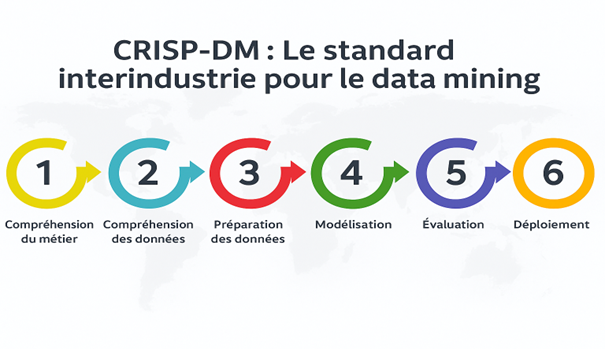
\includegraphics[width=0.65\textwidth]{crisp_dm.png}

  \caption{Cycle de vie du framework CRISP-DM}
  \label{fig:crisp_dm}
\end{figure}

\begin{enumerate}[leftmargin=*, label=\arabic*.]
  \item \textbf{Compréhension métier (\textit{Business Understanding}) :} Définir les
        objectifs du projet et traduire les objectifs métier en problèmes de fouille de
        données.
  \item \textbf{Compréhension des données (\textit{Data Understanding}) :} Collecter les
        données initiales, évaluer leur qualité et découvrir des premières perspectives.
  \item \textbf{Préparation des données (\textit{Data Preparation}) :} Nettoyer,
        transformer et mettre en forme les données pour les besoins de la modélisation.
  \item \textbf{Modélisation (\textit{Modeling}) :} Sélectionner et appliquer des
        techniques de modélisation avec des paramètres optimisés.
  \item \textbf{Évaluation (\textit{Evaluation}) :} Évaluer les résultats du modèle par
        rapport aux objectifs métier et aux critères de succès.
  \item \textbf{Déploiement (\textit{Deployment}) :} Mettre en production les résultats
        et établir une stratégie de surveillance continue.
\end{enumerate}

\paragraph{Avantages de CRISP-DM}
\begin{itemize}[leftmargin=*, label=\textbullet]
  \item \textbf{Orienté métier :} Démarre par la compréhension métier, en parfait
        alignement avec les besoins d'entreprise tels que l'interprétation des anomalies
        SAP et l'analyse d'impact.
  \item \textbf{Workflow itératif :} Encourage les retours continus et le raffinement du
        modèle, utile pour améliorer la précision et la pertinence des alertes.
  \item \textbf{Neutre technologiquement :} N'impose pas de contraintes d'outillage, bien
        adapté à une intégration flexible avec des stacks modernes.
  \item \textbf{Largement adopté :} Éprouvé par l'industrie et soutenu par une
        documentation et des outils abondants.
  \item \textbf{Accent sur l'évaluation :} Inclut des phases dédiées à l'évaluation de
        la performance technique et de l'adéquation métier, essentielles pour les
        applications de surveillance SAP.
\end{itemize}

\paragraph{Limites de CRISP-DM}
\begin{itemize}[leftmargin=*, label=\textbullet]
  \item \textbf{Absence de MLOps intégré :} Ne traite pas nativement les pratiques de
        déploiement modernes (CI/CD, versionnage, surveillance).
\end{itemize}

\subsubsection{KDD – Knowledge Discovery in Databases}

Le processus KDD (\textit{Knowledge Discovery in Databases}), introduit par Fayyad et al.
en 1996, est l'une des premières méthodologies formelles pour extraire des connaissances
actionnables de larges volumes de données. Il met l'accent sur le cycle de vie complet,
de la préparation des données jusqu'à l'interprétation des connaissances.

\begin{figure}[htbp]
  \centering
   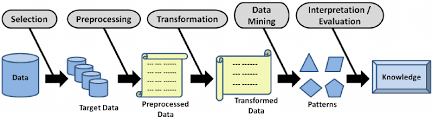
\includegraphics[width=0.65\textwidth]{kdd.png}

  \caption{Étapes du processus KDD}
  \label{fig:kdd}
\end{figure}

\paragraph{Avantages}
\begin{itemize}[leftmargin=*, label=\textbullet]
  \item Fort accent sur la validité, la nouveauté et l'utilité des connaissances.
  \item Promeut un pipeline d'analyse de données complet et itératif.
\end{itemize}

\paragraph{Inconvénients}
\begin{itemize}[leftmargin=*, label=\textbullet]
  \item Guidance limitée sur le déploiement ou l'opérationnalisation.
  \item Moins d'accent sur les pratiques agiles ou les principes d'ingénierie logicielle.
\end{itemize}

\subsubsection{TDSP – Team Data Science Process}

Le TDSP (\textit{Team Data Science Process}) est un framework développé par Microsoft
pour guider les projets de data science. Son cycle de vie comprend cinq étapes itératives,
similaires à celles de CRISP-DM (voir Figure~\ref{fig:tdsp}).

\begin{figure}[htbp]
  \centering
   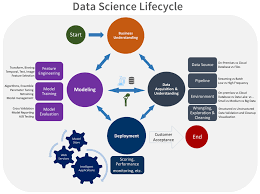
\includegraphics[width=0.65\textwidth]{tdsp (1).png}

  \caption{Cycle de vie de la méthodologie Microsoft TDSP}
  \label{fig:tdsp}
\end{figure}

\begin{enumerate}[leftmargin=*, label=\arabic*.]
  \item \textbf{Compréhension métier :} Définir les objectifs et identifier les sources
        de données.
  \item \textbf{Acquisition et compréhension des données :} Ingérer les données et
        déterminer si elles peuvent répondre à la question posée.
  \item \textbf{Modélisation :} Ingénierie des fonctionnalités et entraînement des
        modèles.
  \item \textbf{Déploiement :} Mise en production dans un environnement opérationnel.
\end{enumerate}

\paragraph{Avantages}
\begin{itemize}[leftmargin=*, label=\textbullet]
  \item \textbf{Agile :} Insiste sur les livrables incrémentaux.
  \item \textbf{Familier :} Backlog produit, user stories, versionnage Git et sprint
        planning familiers aux équipes habituées aux pratiques logicielles courantes.
  \item \textbf{Natif data science :} Reconnaît les différences entre data science et
        ingénierie logicielle.
  \item \textbf{Flexible :} Peut être implémenté seul ou combiné avec d'autres approches.
\end{itemize}

\paragraph{Inconvénients}
\begin{itemize}[leftmargin=*, label=\textbullet]
  \item \textbf{Sprints fixes :} De nombreux data scientists peinent avec les sprints de
        durée fixe imposés par TDSP.
  \item \textbf{Quelques incohérences :} La documentation Microsoft n'est pas toujours
        parfaitement cohérente.
\end{itemize}

\subsection{Comparaison des méthodologies}

\begin{table}[htbp]
  \centering
  \caption{Comparaison des méthodologies CRISP-DM, TDSP et KDD}
  \label{tab:methodo_comparison}
  \begin{tabularx}{\textwidth}{>{\bfseries}p{3.2cm} X X X}
    \toprule
    \textbf{Aspect} & \textbf{CRISP-DM} & \textbf{TDSP} & \textbf{KDD} \\
    \midrule
    Objectif principal & Processus structuré et itératif pour la fouille de données orientée métier & Cycle de vie agile pour projets ML scalables & Extraction de patterns et connaissances depuis des données brutes \\
    \midrule
    Intégration métier & Forte : la compréhension métier est le point de départ & Forte : phase d'alignement intégré & Limitée : orientée données et patterns \\
    \midrule
    Préparation des données & Extensive et itérative & Forte, souvent automatisée & Phase centrale \\
    \midrule
    Support à la modélisation & Sélection et ajustement de modèles inclus & Fort avec suivi de performance & Présent mais moins structuré \\
    \midrule
    Support au déploiement & Modéré : inclus mais peu prescriptif & Fort : accent sur la production et DevOps & Minimal \\
    \midrule
    Interprétabilité & Soulignée lors de l'évaluation & Modérée : axée sur la reproductibilité & Haute : les patterns doivent être compréhensibles \\
    \midrule
    Meilleur cas d'usage & Fouille de données avec contexte métier fort & Flux ML collaboratifs et itératifs & Découverte de connaissances dans des données brutes non étiquetées \\
    \bottomrule
  \end{tabularx}
\end{table}

\subsection{Méthodologie retenue : CRISP-DM}

\textbf{CRISP-DM} a été adoptée comme méthodologie principale de ce projet en raison de
son alignement métier, de sa neutralité technologique et de son accent sur l'amélioration
itérative — une exigence clé pour la construction d'un assistant de surveillance SAP
utilisable et adaptable.

% ============================================================
\section*{Conclusion}
\addcontentsline{toc}{section}{Conclusion}

Ce chapitre a mis en évidence l'importance stratégique du développement d'un système
de détection d'anomalies SAP répondant aux lacunes critiques des approches de
surveillance actuelles. Grâce à la méthodologie CRISP-DM, le projet vise à transformer
la surveillance SAP réactive en une détection d'anomalies proactive et contextualisée.
La solution proposée, basée sur une architecture hybride RAG enrichie par des graphes de
connaissances, constitue une réponse innovante aux limites des outils existants, tout en
s'appuyant sur des technologies open source accessibles et performantes.
% ============================================================
%  Chapitre 2 : Compréhension métier et spécification des besoins
% ============================================================

\chapter{Compréhension métier et spécification des besoins}
\label{chap:business_understanding}

\section*{Introduction}
\addcontentsline{toc}{section}{Introduction}

Ce chapitre présente le contexte métier et les objectifs du projet d'assistant
intelligent de surveillance SAP dans le cadre de la méthodologie CRISP-DM. Il met en
évidence l'importance d'aligner les efforts techniques sur les objectifs métier, afin
que la solution développée réponde aux défis réels auxquels sont confrontées les équipes SAP.

Avant de commencer la phase de réalisation, il est crucial de bien définir les contours du système à mettre en place. Ce chapitre jette les bases du projet en identifiant les attentes des utilisateurs, en précisant les fonctionnalités requises et en établissant les contraintes à respecter. La méthodologie CRISP-DM oriente cette démarche structurée, depuis la compréhension du domaine jusqu'à la conception d'une solution appropriée pour le contexte de surveillance SAP d'Avaxia Group.

% ============================================================
\section{Contexte métier SAP}
\label{sec:contexte_sap}

\subsection{Qu'est-ce qu'un ERP ?}

Un système ERP (\textit{Enterprise Resource Planning}) est un logiciel qui intègre et
gère les principaux processus métier d'une organisation : finances, ressources humaines,
fabrication, chaîne d'approvisionnement, ventes et achats. Il fournit une source unique
de vérité, élimine la duplication des données et améliore l'efficacité opérationnelle.
Les solutions ERP permettent aux entreprises d'obtenir une visibilité en temps réel sur
leurs opérations, d'automatiser les processus et de prendre des décisions basées sur
les données.

\textbf{SAP} (\textit{Systems, Applications and Products in Data Processing}) est l'un
des principaux fournisseurs de logiciels ERP. Sa suite logicielle couvre de nombreux
domaines fonctionnels. Parmi ses modules les plus utilisés :

\begin{itemize}[leftmargin=*, label=\textbullet]
  \item \textbf{SAP EWM (\textit{Extended Warehouse Management}) :} Module spécialisé
        dans l'optimisation des entrepôts et la gestion des stocks. Il aide les entreprises
        à gérer efficacement leurs opérations d'entreposage et à garantir la disponibilité
        des produits au bon moment.
  \item \textbf{SAP ECC (\textit{Enterprise Central Component}) :} Module central de
        l'ERP SAP. Il intègre les finances, les ventes, les achats, la fabrication et
        les ressources humaines au sein d'une plateforme unifiée.
  \item \textbf{SAP Solution Manager (SOLMAN) :} Outil central de gestion et de
        surveillance fourni par SAP. Il couvre la gestion du cycle de vie des applications,
        la gestion de projets, la gestion des services IT et le suivi des processus métier.
\end{itemize}

\begin{figure}[H]
  \centering
  
\includegraphics[width=0.15\textwidth]{images/SAP_2011_logo.svg}
  \caption{Logo SAP}
  \label{fig:sap_logo}
\end{figure}

% ============================================================
\subsection{Le consultant SAP BASIS}

Le consultant SAP BASIS est responsable de l'infrastructure technique de l'environnement SAP : installations, mises à jour et application des correctifs. Il assure la résolution des problèmes de connectivité, les ajustements de composants et l'assistance aux systèmes externes et aux bases de données.

Ses principales responsabilités englobent l'administration des systèmes, la surveillance des performances, la sécurité et la gestion des bases de données, ainsi que la résolution des incidents techniques.

Il prend également en charge la sauvegarde et la récupération des données, la gestion des intégrations et des interfaces, les mises à jour et migrations des systèmes, et veille à maintenir une documentation à jour tout en assurant la formation des équipes concernées.

Dans le cadre du suivi opérationnel, il surveille en continu les performances et le bon fonctionnement des systèmes SAP à l'aide des transactions \textit{(T-Codes)} dédiées, et applique les correctifs nécessaires via les \textit{SAP Notes} afin de garantir la stabilité et la fiabilité de l'environnement.

% ============================================================
\subsection{Les codes de transaction SAP (T-codes)}

Dans SAP, les codes de transaction (T-codes) sont des commandes alphanumériques courtes
permettant d'accéder rapidement à des fonctions spécifiques, des rapports ou des
diagnostics système. Ils servent de points d'entrée dans les modules fonctionnels de SAP,
permettant aux utilisateurs de contourner les menus profonds et d'exécuter directement
des tâches telles que la surveillance des jobs, la gestion des files d'attente ou
l'analyse des performances.

Chaque T-code correspond à une fonction ou un programme backend : généralement implémenté
en ABAP : qui effectue un ensemble défini d'opérations. Lors de l'exécution d'un T-code,
SAP vérifie les autorisations de l'utilisateur, exécute la logique associée et présente
une interface interactive.

Dans le cadre de ce projet, un ensemble de T-codes à haute criticité a été sélectionné
pour assurer une couverture complète du comportement des systèmes SAP :

\begin{itemize}[leftmargin=*, label=\textbullet]
  \item \texttt{ST22} – Analyse des erreurs d'exécution ABAP (\textit{short dumps}).
  \item \texttt{DB02} – Surveillance des statistiques de base de données (croissance,
        espace table, index manquants).
  \item \texttt{SM37} – Surveillance des jobs en arrière-plan.
  \item \texttt{SP01} – Vérification des requêtes d'impression et de leurs statuts.
  \item \texttt{SM66} – Vue globale des processus de travail actifs.
  \item \texttt{SM58} – Analyse des erreurs RFC transactionnelles (traitement asynchrone).
  \item \texttt{SMQ1}, \texttt{SMQ2} – Surveillance des files d'attente entrantes et
        sortantes (qRFC/tRFC).
  \item \texttt{SM12}, \texttt{SM13} – Révision des entrées verrouillées et des
        enregistrements de mise à jour.
  \item \texttt{ST03N} – Analyse des statistiques de charge de travail et de performance.
  \item \texttt{SOST} – Surveillance des messages SAPconnect (e-mails, fax, etc.).
  \item \texttt{ST13} – Outils BASIS pour les diagnostics approfondis et les journaux.
\end{itemize}

Ces T-codes ont été sélectionnés en raison de leur criticité pour les opérations en temps
réel, de leur pertinence pour les équipes BASIS et de leur fréquence d'utilisation lors
de la résolution des incidents. En s'appuyant sur la documentation officielle de ces
transactions et sur les SAP Notes associées, le système permet aux consultants BASIS de
retrouver rapidement les procédures d'analyse et de résolution applicables à chaque
erreur observée.

\subsubsection*{SM37 : Job Overview}

SM37 surveille les \textit{jobs batch} — ce sont des tâches automatiques qui
tournent en arrière-plan (traitements de données, interfaces, rapports).
L'administrateur vérifie qu'aucun job n'est en erreur ou bloqué.

\begin{figure}[H]
  \centering
  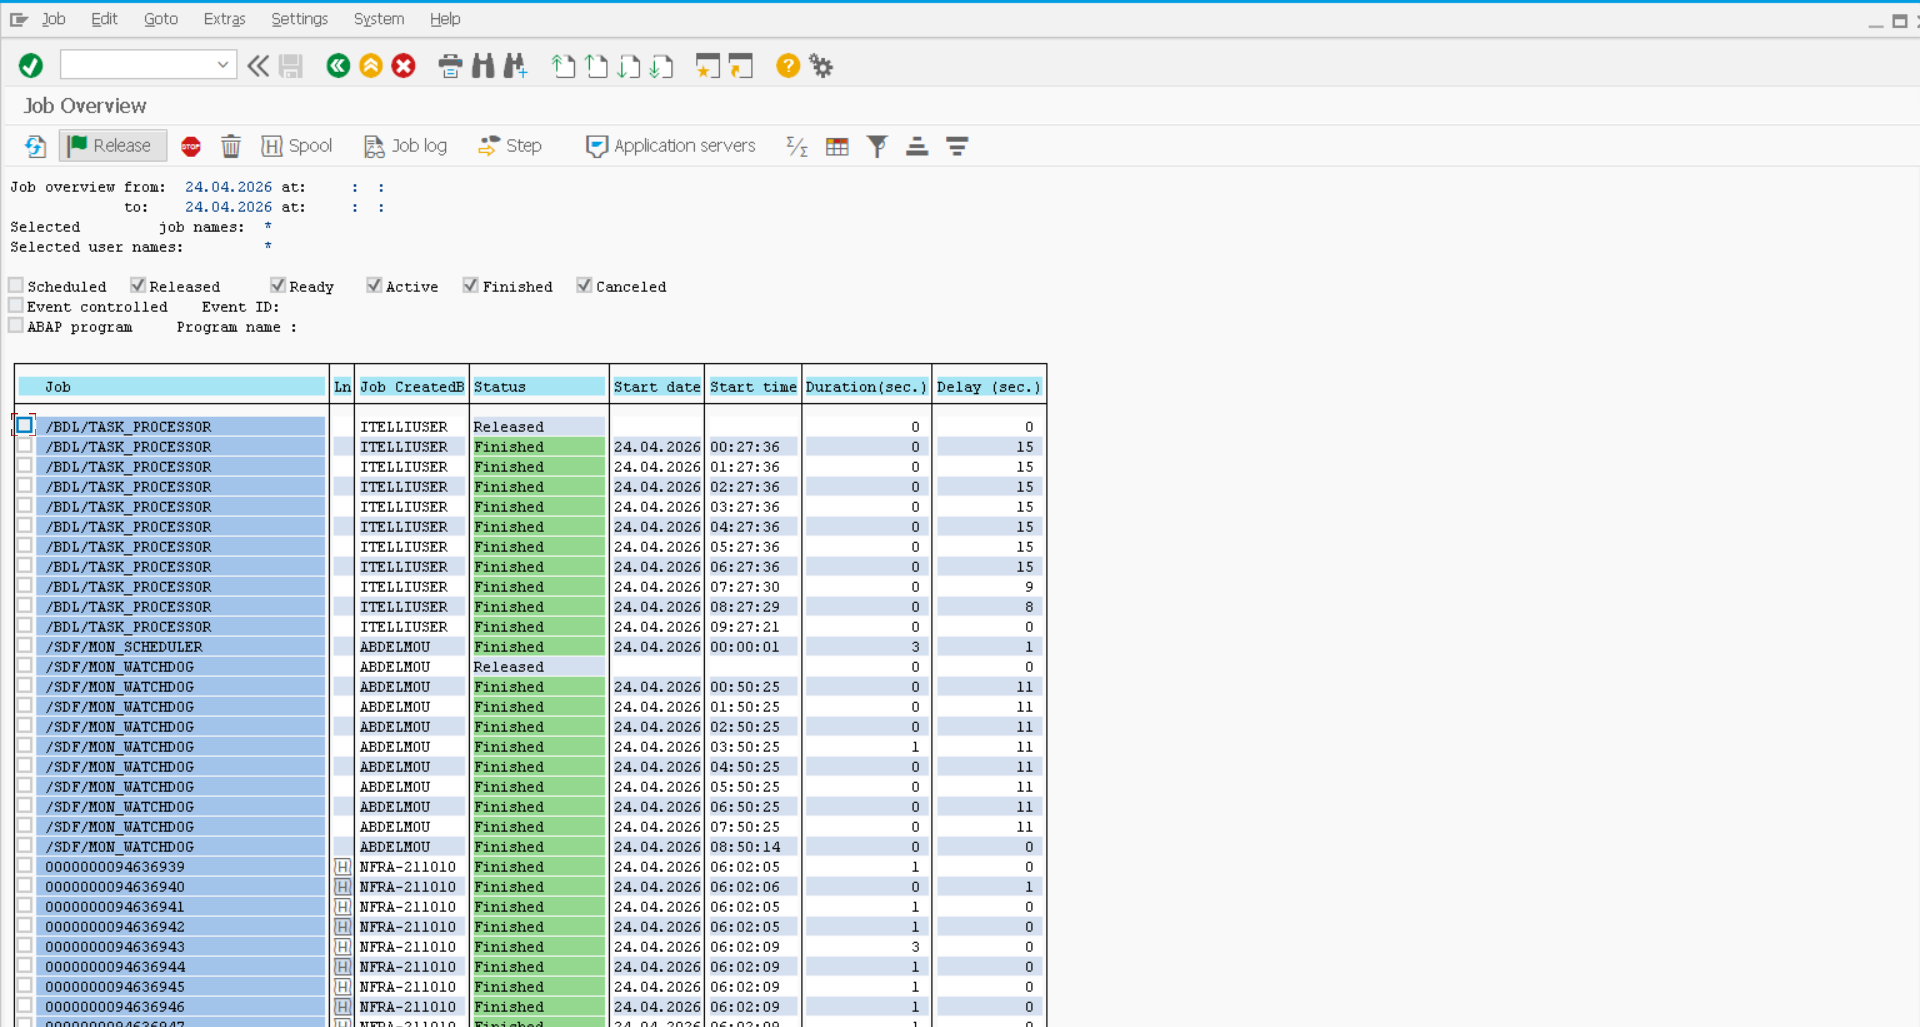
\includegraphics[width=\textwidth]{images/sm37.png}
  \caption{SM37 : Vue d'ensemble des jobs batch}
  \label{fig:sm37}
\end{figure}

La figure~\ref{fig:sm37} présente l'interface du T-code \texttt{SM37}, qui affiche
la liste des jobs planifiés avec leur statut (\textit{Finished}, \textit{Released},
\textit{Active}), leur date et heure de démarrage, leur durée d'exécution ainsi que
le délai éventuel. Cette vue permet à l'administrateur BASIS d'identifier en un coup
d'œil tout job bloqué, annulé ou présentant un délai anormal, et d'intervenir
rapidement avant que cela n'impacte les processus métier.

\subsubsection*{DB02 : Space Overview}

DB02 surveille la base de données ; l'administrateur contrôle l'espace disque
disponible pour éviter que la base de données sature, ce qui provoquerait un
arrêt complet du système.

\begin{figure}[H]
  \centering
  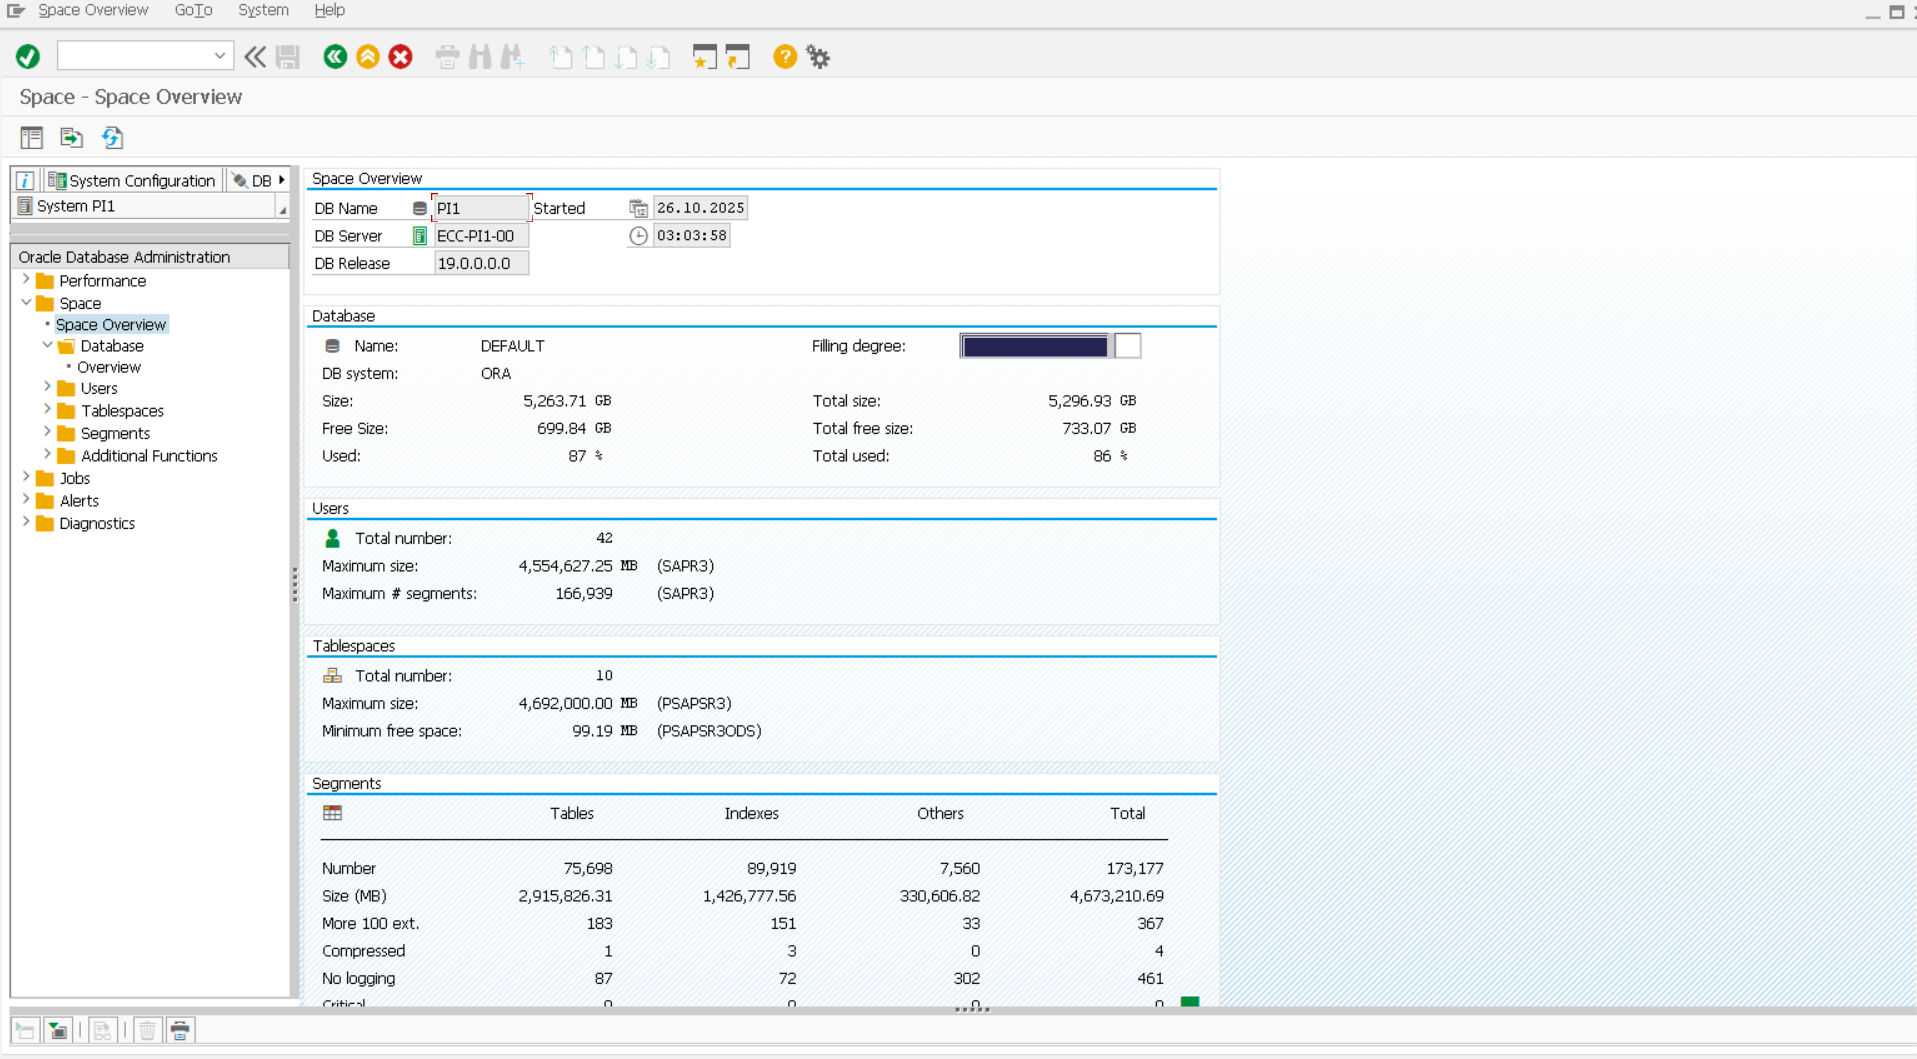
\includegraphics[width=\textwidth]{images/db02.png}
  \caption{DB02 : Vue d'ensemble de l'espace base de données}
  \label{fig:db02}
\end{figure}

La figure~\ref{fig:db02} illustre le T-code \texttt{DB02}, qui fournit une vue
synthétique de l'état de la base de données Oracle. On y retrouve le taux de
remplissage global, la taille totale et l'espace libre, ainsi que le détail par
tablespace et par segment (tables, index, autres). Un taux d'utilisation élevé
comme les 87\% visibles ici : constitue un signal d'alerte critique nécessitant
une action immédiate d'extension ou de purge pour prévenir toute saturation du système.

\subsubsection*{ST22 : Runtime Errors}

ST22 liste les erreurs critiques ABAP : l'administrateur analyse les
\textit{dumps} pour identifier les programmes qui plantent et corriger
les problèmes avant qu'ils n'impactent les utilisateurs.

\begin{figure}[H]
  \centering
  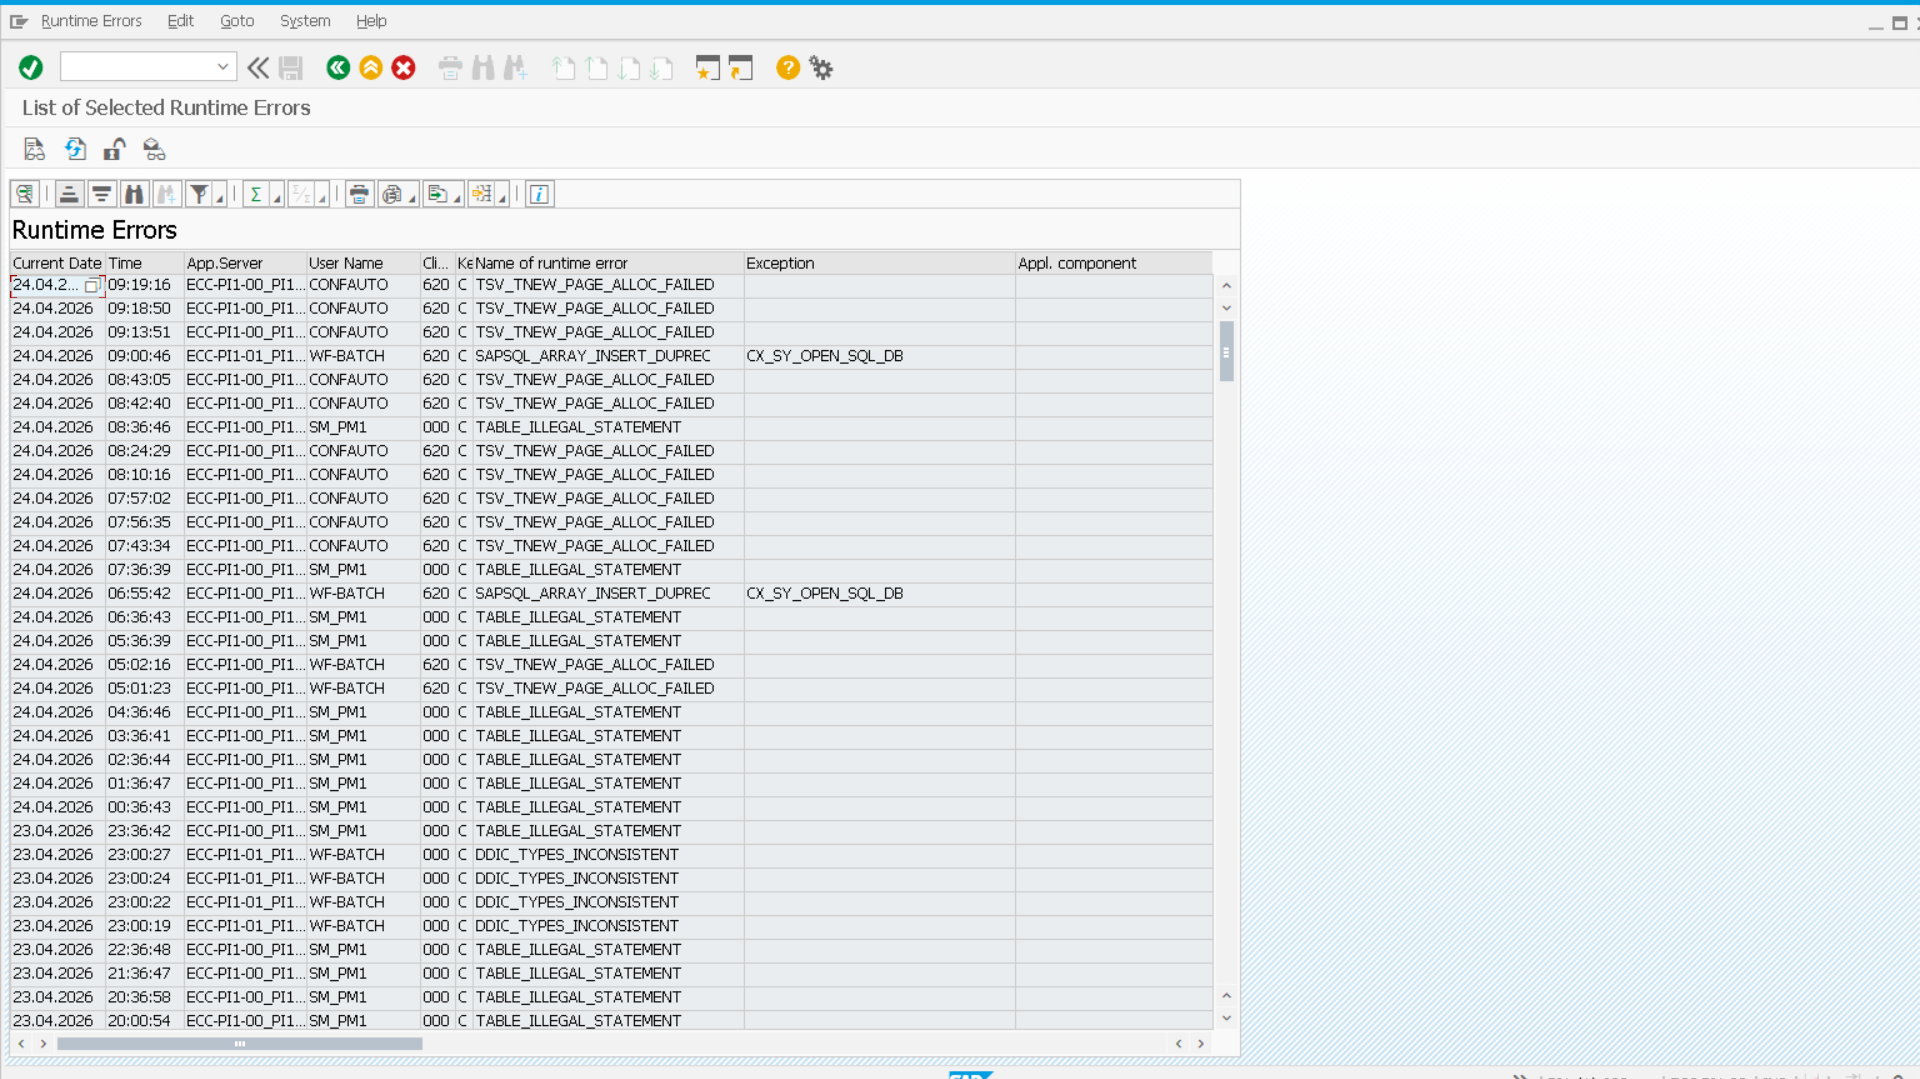
\includegraphics[width=\textwidth]{images/st22.png}
  \caption{ST22 : Liste des erreurs d'exécution ABAP}
  \label{fig:st22}
\end{figure}

La figure~\ref{fig:st22} présente l'interface du T-code \texttt{ST22}, qui recense
l'ensemble des \textit{short dumps} ABAP survenus sur le système. Chaque entrée
indique la date, l'heure, le serveur applicatif, l'utilisateur concerné et le nom
de l'erreur. Les erreurs récurrentes telles que \texttt{TSV\_TNEW\_PAGE\_ALLOC\_FAILED}
(manque de mémoire) ou \texttt{TABLE\_ILLEGAL\_STATEMENT} (instruction SQL non autorisée)
sont des indicateurs d'anomalies systémiques qui doivent être analysées et résolues
en priorité par l'équipe BASIS.

% ─────────────────────────────────────────────────────────────
\section{Vision et objectifs du système futur}
% ─────────────────────────────────────────────────────────────

Dans le cadre de l'optimisation et de la modernisation de l'exploitation des systèmes SAP, le projet vise à développer un assistant intelligent capable d'analyser et d'exploiter de manière efficace les données issues des différentes transactions et opérations. Les principaux objectifs du système futur sont les suivants :

\begin{itemize}
    \item \textbf{Centraliser et organiser les données SAP} provenant des différents modules, afin de disposer d'une source unique et fiable d'informations.
    \item \textbf{Analyser et interpréter les incidents} grâce à un assistant intelligent qui retrouve et présente les procédures de diagnostic et de résolution adaptées au contexte SAP de l'utilisateur.
    \item \textbf{Faciliter l'analyse des incidents} en fournissant rapidement, à partir d'un T-code ou d'un message d'erreur, les sections de documentation et les SAP Notes pertinentes pour leur résolution.
    \item \textbf{Exploiter le corpus documentaire SAP} grâce à un pipeline de recherche sémantique et lexicale (RAG hybride), produisant des réponses sourcées et vérifiables en langage naturel.
    \item \textbf{Offrir une interface interactive} sous forme d'assistant conversationnel permettant aux utilisateurs de poser des questions, d'obtenir des analyses et de recevoir des conseils personnalisés.
    \item \textbf{Assurer une accessibilité via une application web} intuitive, permettant de visualiser les analyses, exploiter les données collectées et interagir avec l'assistant de manière ergonomique.
\end{itemize}

Ainsi, ce système contribuera à améliorer la compréhension et la gestion des données SAP, à faciliter l'analyse des anomalies, et à offrir un outil intelligent d'aide à la décision pour les utilisateurs.

% ─────────────────────────────────────────────────────────────
\section{Spécification des besoins}
\label{sec:specification_besoins}
% ─────────────────────────────────────────────────────────────

L'analyse des besoins a pour objectif de comprendre les attentes des utilisateurs et de définir le
contexte métier dans lequel s'inscrit le système à développer. Elle permet de décrire
les fonctionnalités que le système prendra en charge, ses interactions avec les différents
intervenants, ainsi que les règles qui encadrent ces interactions.

\subsection{Identification des acteurs}

Pour déterminer les besoins fonctionnels et non fonctionnels, nous débutons par
l'identification des acteurs impliqués dans le système, en précisant le rôle spécifique
de chacun. Ainsi, nous identifions trois rôles distincts qui interagissent avec le
système :

\begin{table}[H]
\centering
\renewcommand{\arraystretch}{1.45}
\caption{Acteurs du système AutoMoni et leurs responsabilités}
\label{tab:acteurs}
\begin{tabularx}{\textwidth}{|p{4.5cm}|p{3.5cm}|X|}
\hline
\textbf{Acteur} & \textbf{Type} & \textbf{Responsabilités principales} \\
\hline
Administrateur SAP (consultant BASIS)
  & Acteur principal
  & Surveille les environnements SAP à travers les données de monitoring collectées en temps réel. Interagit avec l'assistant intelligent pour poser des questions techniques en langage naturel, consulter les alertes T-code, accéder aux journaux de transactions et visualiser les graphiques d'analyse. Configure les paramètres de surveillance et de la plateforme AutoMoni. Soumet des feedbacks sur les réponses du chatbot afin d'améliorer la qualité du système RAG. Cumule l'ensemble des privilèges de l'Utilisateur SAP. \\
\hline
Utilisateur SAP
  & Acteur principal
  & Consulte les pages de monitoring SAP, interagit avec l'assistant intelligent via la page chatbot ou le panneau latéral, pose des questions en langage naturel, navigue vers les pages T-code depuis le chatbot et consulte l'historique de ses conversations. \\
\hline
Système SAP (source externe)
  & Acteur secondaire
  & Fournit les données de surveillance opérationnelle via les appels RFC (PyRFC). Ne déclenche pas d'interactions directes avec l'interface, mais alimente en continu la base de données de monitoring interrogée par les acteurs humains. \\
\hline
\end{tabularx}
\end{table}

\subsection{Besoins fonctionnels}

Les besoins fonctionnels définissent l'ensemble des fonctionnalités que le système doit
fournir afin de permettre aux utilisateurs d'exploiter et d'analyser les données issues
de l'environnement SAP à travers un assistant intelligent basé sur l'intelligence
artificielle et reposant sur une architecture de génération augmentée par récupération
\textit{(RAG -- Retrieval-Augmented Generation)}.

Le système repose sur deux types d'acteurs principaux : l'\textbf{Administrateur SAP}
et l'\textbf{Utilisateur SAP}. Il convient de préciser que l'administrateur SAP englobe
l'ensemble des privilèges de l'utilisateur SAP : en plus de ses responsabilités de
supervision et de configuration, il peut également interagir avec l'assistant intelligent
et exploiter pleinement les fonctionnalités offertes par le module RAG, au même titre
qu'un utilisateur standard.

\subsubsection*{Administrateur SAP}

L'administrateur occupe un rôle central de supervision et de gouvernance de la plateforme AutoMoni.
En tant qu'acteur disposant des droits les plus étendus, il cumule l'ensemble des fonctionnalités
de l'utilisateur SAP, auxquelles s'ajoutent ses responsabilités d'administration.
Ses responsabilités spécifiques sont les suivantes~:

\begin{itemize}
  \item Interagir avec l'assistant intelligent RAG via la page chatbot dédiée ou le tiroir
        latéral accessible depuis toutes les pages.
  \item Formuler des requêtes en langage naturel sur les données SAP et recevoir des réponses
        vérifiées accompagnées de leurs sources documentaires.
  \item Naviguer automatiquement vers une page de monitoring en mentionnant un T-code dans le chatbot.
  \item Soumettre un retour (\textit{feedback}) sur les réponses générées afin d'améliorer
        la qualité du pipeline RAG.
\end{itemize}

\subsubsection*{Utilisateur SAP}

L'utilisateur SAP constitue l'acteur principal de l'application AutoMoni.
Il peut exploiter les fonctionnalités suivantes~:

\begin{itemize}
  \item S'authentifier à l'application.
  \item Consulter les pages de monitoring SAP correspondant aux T-codes de surveillance.
  \item Interagir avec l'assistant intelligent via la page chatbot dédiée ou via le panneau
        latéral coulissant disponible sur toutes les pages.
  \item Poser des questions en langage naturel sur les données issues du système SAP.
  \item Naviguer vers une page de monitoring en mentionnant un T-code dans le chatbot.
  \item Consulter les sources documentaires et les avertissements associés à chaque réponse.
  \item Consulter l'historique de ses propres interactions avec le chatbot.
\end{itemize}

\subsection{Besoins non fonctionnels}

Les besoins non fonctionnels définissent les critères de qualité mesurables que le système doit respecter. Ils constituent les \textit{Business Success Criteria} de la phase Business Understanding de CRISP-DM et seront confrontés aux mesures du chapitre~6.

\subsubsection{Performance}

Le pipeline complet (retrieval + génération) doit retourner une réponse en moins de 5 secondes pour 95\,\% des requêtes (P95 $\leq$ 5\,s). Ce seuil justifie le choix de l'index HNSW (recherche en $O(\log n)$) et le déploiement local du LLM via Ollama.

\subsubsection{Fiabilité}

Le taux d'hallucination doit rester inférieur à 5\,\%, garanti par une validation déterministe par règles~: les T-codes SAP et numéros de SAP Notes mentionnés dans la réponse sont comparés par expressions régulières à ceux présents dans les chunks récupérés~; toute entité non ancrée est supprimée avant renvoi (cf.\ §\,5.9.5 et §\,6.7).

\subsubsection{Confidentialité}

L'intégralité du pipeline tourne en local — LLM via Ollama, base vectorielle via PostgreSQL/pgvector. Aucune donnée SAP n'est transmise à des APIs cloud externes.

\subsubsection{Scalabilité}

L'index HNSW supporte l'insertion incrémentale sans reconstruction, ce qui permet d'ajouter de nouvelles SAP Notes ou de nouveaux modules sans réindexer l'intégralité du corpus.

\begin{table}[H]
\centering
\renewcommand{\arraystretch}{1.3}
\caption{Synthèse des besoins non fonctionnels}
\label{tab:nfr_synthese}
\begin{tabularx}{\textwidth}{|p{3cm}|p{4cm}|X|}
\hline
\textbf{Catégorie} & \textbf{Seuil cible} & \textbf{Mécanisme de garantie} \\
\hline
Performance & P95 $\leq$ 5\,s & Index HNSW + LLM local Ollama \\
\hline
Fiabilité & Taux d'hallucination $<$ 5\,\% & Validation ensembliste des T-codes et SAP Notes (§\,5.9.5, §\,6.7) \\
\hline
Confidentialité & 0 donnée transmise à des APIs cloud & Pipeline 100\,\% local (Ollama + pgvector) \\
\hline
Scalabilité & Insertion sans réindexation & Index HNSW incrémental (PostgreSQL pgvector) \\
\hline
\end{tabularx}
\end{table}

\subsection{Diagramme de cas d'utilisation général}

La figure~\ref{fig:usecase_deploy} synthétise les interactions entre les acteurs identifiés et les fonctionnalités du système. L'Administrateur SAP cumule les privilèges de l'Utilisateur SAP et y ajoute la configuration de la plateforme. L'Utilisateur SAP peut consulter les pages de monitoring, interroger l'assistant et naviguer automatiquement vers les pages T-code mentionnées dans les réponses.

\begin{figure}[H]
    \centering
    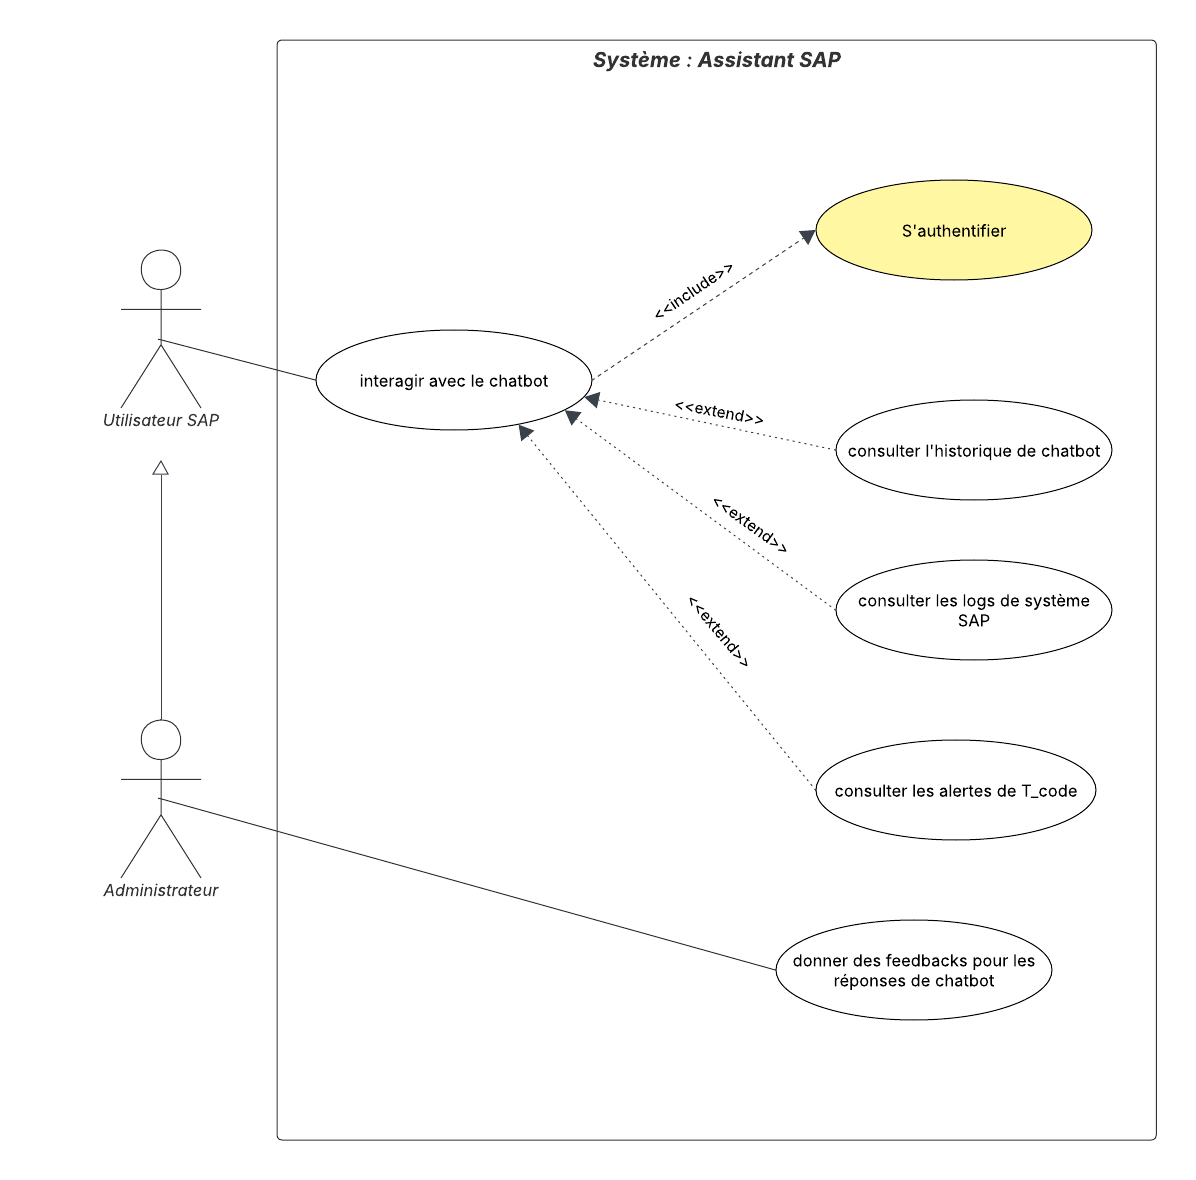
\includegraphics[width=0.9\textwidth]{images/casutilisation.png}
    \caption[Diagramme de cas d'utilisation]{Diagramme de cas d'utilisation général du système}
    \label{fig:usecase_deploy}
\end{figure}

% ============================================================
\section{État de l'art}
\label{sec:etat_art}

\subsection{Les Fondements Technologiques de l'IA Générative}

L'intelligence artificielle générative repose sur un ensemble de technologies complémentaires qui, combinées, permettent de concevoir des systèmes capables d'analyser, de raisonner et de produire du contenu à partir de données complexes. Cette section présente les principaux fondements technologiques qui soutiennent la compréhension et la génération du langage naturel.

Elle introduit tout d'abord les concepts essentiels de l'apprentissage automatique (\textit{Machine Learning}) et de l'intelligence artificielle, avant d'explorer l'apprentissage profond (\textit{Deep Learning}) ainsi que les modèles basés sur l'architecture \textit{Transformer}. Elle aborde ensuite le traitement automatique du langage naturel (\textit{NLP -- Natural Language Processing}) et met en lumière l'émergence des modèles de langage de grande taille (\textit{LLMs -- Large Language Models}), qui jouent un rôle central dans la génération de texte. Enfin, l'architecture \textit{RAG (Retrieval-Augmented Generation)} est présentée comme une approche permettant d'enrichir ces modèles en leur fournissant un accès à des connaissances actualisées et vérifiables. L'ensemble de ces technologies constitue le socle sur lequel repose la solution proposée dans ce projet.

\subsection{Machine Learning et Intelligence Artificielle}

Le \textit{Machine Learning}, ou apprentissage automatique, constitue l'un des piliers fondamentaux de l'intelligence artificielle. Il permet à un système d'apprendre à partir de données sans être explicitement programmé pour chaque tâche. En analysant des ensembles de données, le modèle identifie des régularités statistiques qu'il utilise pour effectuer des prédictions sur de nouvelles données. Cette capacité d'apprentissage automatique est à la base des avancées récentes en intelligence artificielle générative.

\subsection{Deep Learning}

L'apprentissage profond (\textit{Deep Learning}) est une sous-discipline du \textit{Machine Learning} qui repose sur des réseaux de neurones artificiels composés de plusieurs couches. Ces réseaux permettent d'extraire progressivement des représentations de plus en plus abstraites des données. Grâce à cette structure, ils sont particulièrement efficaces pour traiter des données non structurées telles que le texte, les images ou encore les signaux audio.

\subsection{Architecture Transformer}

Proposée en 2017 dans l'article \textit{« Attention is All You Need »} \cite{vaswani2017attention}, l'architecture \textit{Transformer} s'est imposée comme une référence dans le domaine du traitement du langage naturel. Elle repose sur le mécanisme d'\textbf{attention} (\textit{self-attention}), qui permet au modèle d'évaluer l'importance de chaque mot par rapport à tous les autres mots d'une séquence, indépendamment de leur position.

Contrairement aux architectures séquentielles traditionnelles telles que les réseaux récurrents (\textit{RNN, LSTM}), le Transformer traite les données en parallèle, ce qui améliore considérablement les performances et permet de capturer efficacement les dépendances à long terme dans le texte.

\subsection{Traitement Automatique du Langage Naturel (NLP)}

Le traitement automatique du langage naturel (\textit{NLP}) est un domaine de l'intelligence artificielle dédié à l'interaction entre les machines et le langage humain. Il regroupe un ensemble de techniques permettant de comprendre, analyser et générer du texte~\cite{jurafsky2024slp}.

Parmi les principales applications du NLP figurent la classification de textes, l'analyse de sentiments, la traduction automatique, la reconnaissance d'entités nommées ainsi que la génération automatique de contenu.

\subsection{Les Modèles de Langage de Grande Taille : Capacités et Limites}

Les modèles de langage de grande taille (\textit{LLMs}) sont des modèles avancés d'apprentissage profond entraînés sur des volumes massifs de données textuelles (livres, articles, sites web, code, etc.). Leur objectif est de comprendre et de générer un langage proche de celui des humains~\cite{brown2020gpt3}.

Comme illustré dans la figure~\ref{fig:llm_intersection}, ces modèles se situent à l'intersection du \textit{Deep Learning} et du \textit{NLP}, combinant ainsi la puissance des réseaux de neurones profonds avec les techniques d'analyse linguistique.

En pratique, un LLM prédit le mot (ou jeton) le plus probable à la suite d'une séquence donnée. En répétant ce processus, il est capable de produire des textes cohérents, de répondre à des questions, de résumer des documents ou encore de traduire des contenus. Plus le modèle contient de paramètres, plus il est capable de capturer les nuances complexes du langage.

\begin{figure}[H]
  \centering
  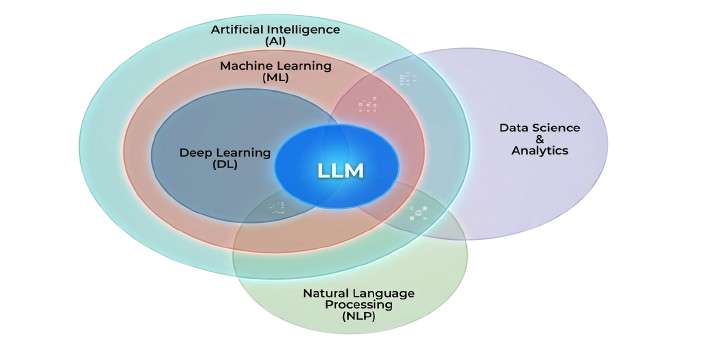
\includegraphics[width=0.6\textwidth]{images/llmv1.png}
  \caption{Les LLMs à l'intersection du \textit{Deep Learning} et du \textit{NLP}}
  \label{fig:llm_intersection}
\end{figure}

Malgré leurs performances impressionnantes, les LLMs présentent certaines limites. Leur connaissance est limitée aux données utilisées lors de leur entraînement, ce qui les empêche de traiter des informations récentes. De plus, ils peuvent générer des \textbf{hallucinations}, c'est-à-dire produire des réponses plausibles mais incorrectes. Enfin, ils n'ont pas accès aux données internes ou confidentielles d'une organisation.

Parmi les modèles les plus connus figurent \textit{GPT-4}, \textit{Claude} et \textit{Gemini}.

\subsection{Architecture de RAG (Retrieval-Augmented Generation)}

Bien que les LLMs possèdent une connaissance générale acquise lors de leur entraînement, ils ne disposent pas d'un accès direct aux données spécifiques d'une organisation ni aux informations les plus récentes. L'architecture \textit{RAG (Retrieval-Augmented Generation)}~\cite{lewis2020rag} a été conçue pour répondre à cette limitation.

Son fonctionnement repose sur plusieurs étapes. Tout d'abord, les documents sont découpés en fragments appelés \textit{chunks}. Chaque fragment est ensuite transformé en un vecteur numérique (\textit{embedding}) représentant son contenu sémantique~\cite{reimers2019sbert}. Ces vecteurs sont stockés dans une base de données vectorielle.

Lorsqu'une requête utilisateur est soumise, le système identifie les fragments les plus pertinents à l'aide d'une mesure de similarité (généralement la similarité cosinus). Ces informations sont ensuite injectées dans le contexte du modèle, qui génère une réponse basée sur des données réelles et vérifiables.

Ainsi, le RAG peut être comparé à un assistant intelligent capable de consulter une base documentaire avant de formuler une réponse, garantissant ainsi une meilleure fiabilité.
\begin{figure}[H]
\centering
\resizebox{\textwidth}{!}{
\begin{tikzpicture}[
    node distance=2.2cm and 1.6cm,
    every node/.style={font=\footnotesize},
    box/.style={
        draw,
        rounded corners=8pt,
        minimum width=2.6cm,
        minimum height=0.9cm,
        align=center,
        line width=0.8pt,
        drop shadow={opacity=0.15}
    },
    arrow/.style={->, line width=0.9pt}
]

% ---- NODES ----
\node[box, fill=SAPLightOrange, draw=SAPOrange] (docs) {Documents};

\node[box, fill=SAPLightBlue, draw=SAPBlue, right=of docs] (chunk) {Chunking};

\node[box, fill=gray!10, draw=black!50, right=of chunk] (query) {User Query};

\node[box, fill=SAPLightGreen, draw=SAPGreen, right=of query] (vectordb) {Vector DB};

\node[box, fill=SAPLightOrange, draw=SAPRed, below=1.8cm of vectordb] (retrieval) {Top-K\\Retrieval};

\node[box, fill=SAPLightOrange, draw=SAPOrange, left=of retrieval] (llm) {LLM};

\node[box, fill=SAPLightBlue, draw=SAPBlue, left=of llm] (response) {Response};

% ---- FLUX ----
\draw[arrow] (docs) -- node[above]{découpage} (chunk);

\draw[arrow] (chunk) -- node[above]{vectorisation} (query);

\draw[arrow, dashed, color=SAPGreen]
(query) -- node[above]{stockage} (vectordb);

\draw[arrow, color=SAPRed]
(vectordb) -- node[right]{} (retrieval);

\draw[arrow] (query) -- (llm);

\draw[arrow, color=SAPOrange]
(retrieval) -- node[above]{contexte} (llm);

\draw[arrow, color=SAPBlue]
(llm) -- node[above]{génération} (response);

\end{tikzpicture}
}
\caption{Architecture du système RAG }
\label{fig:rag_compact}
\end{figure}

\subsection{L'architecture de CAG (Cache-Augmented Generation) : une amélioration du RAG}

Bien que l'architecture RAG améliore significativement la génération de réponses en intégrant des documents externes, elle présente encore certaines limites, notamment en termes de latence et de coût de calcul, dues aux requêtes répétées vers la base vectorielle.

Pour répondre à ces contraintes, une évolution appelée \textit{CAG (Cache-Augmented Generation)}~\cite{chan2024cag} a été proposée. Le principe de cette approche repose sur l'introduction d'un mécanisme de cache intelligent permettant de stocker les résultats des requêtes précédentes ainsi que les documents fréquemment récupérés.

Ainsi, lorsqu'une requête similaire est posée, le système peut réutiliser directement les informations déjà calculées sans solliciter à nouveau la base vectorielle ou les modèles d'embedding. Cela permet de réduire le temps de réponse et d'améliorer l'efficacité globale du système.

En comparaison avec le RAG classique, le CAG optimise le processus de génération en réduisant les redondances de calcul tout en conservant la pertinence des informations fournies. Cette approche est particulièrement utile dans les systèmes à forte charge ou dans les applications nécessitant une réponse en temps réel.

\subsection{L'architecture de Fine-Tuning : personnalisation des modèles IA}

En plus des approches RAG et CAG, le \textit{Fine-Tuning} est une autre méthode souvent utilisée pour améliorer les performances des modèles d'intelligence artificielle~\cite{devlin2019bert}. Cette technique consiste à ré-entraîner un modèle de langage préexistant sur des données propres à un domaine ou à une organisation.

Le Fine-Tuning permet au modèle d'acquérir le vocabulaire métier, les structures de données et les connaissances spécifiques à une entreprise. Le Fine-Tuning, à la différence du RAG qui récupère des informations externes dynamiquement au moment de la requête, intègre directement ces connaissances dans les paramètres internes du modèle.

Cette approche a plusieurs avantages, notamment une meilleure spécialisation du modèle, une génération de réponses plus cohérente et une réduction de la dépendance aux bases documentaires externes. Mais, elle demande beaucoup de ressources lors de l'entraînement, des mises à jour fréquentes des données et un coût de calcul plus lourd.

\subsection{Comparaison des approches Fine-Tuning, RAG et CAG}

Afin de mieux positionner ces trois approches les unes par rapport aux autres, il convient de les comparer selon plusieurs critères déterminants. Chacune d'elles présente un profil distinct en termes de flexibilité, de coût et de précision. Le Fine-Tuning offre une très haute spécialisation métier, mais au prix d'un entraînement coûteux et d'une mise à jour manuelle des connaissances. Le RAG classique permet une adaptation dynamique aux nouvelles informations grâce à la base documentaire, mais peut souffrir de latences liées aux requêtes vectorielles répétées. Le RAG enrichi du mécanisme de cache (CAG) combine la pertinence documentaire du RAG avec une réduction significative des délais de calcul, ce qui le rend particulièrement adapté aux environnements à forte charge comme les systèmes SAP en production. Le tableau~\ref{tab:comparaison_rag_cag_finetuning} synthétise cette comparaison selon les principaux critères d'évaluation.

\begin{table}[H]
\centering
\renewcommand{\arraystretch}{1.4}
\resizebox{\textwidth}{!}{
\begin{tabular}{|p{3.2cm}|p{3.8cm}|p{3.8cm}|p{4cm}|}
\hline
\textbf{Critère} & \textbf{Fine-Tuning} & \textbf{RAG} & \textbf{RAG + CAG (RAG avancé)} \\
\hline

Principe &
Réentraîner le modèle sur des données spécifiques &
Récupération dynamique de documents pertinents &
RAG avec mécanisme de cache intelligent \\
\hline

Accès aux données récentes &
Limité après l'entraînement &
Oui &
Oui avec optimisation du cache \\
\hline

Temps de réponse &
Rapide &
Moyen &
Très rapide \\
\hline

Coût de calcul &
Élevé lors de l'entraînement &
Modéré &
Optimisé grâce au cache \\
\hline

Mise à jour des connaissances &
Nécessite un nouvel entraînement &
Automatique via la base documentaire &
Automatique avec réutilisation des résultats \\
\hline

Précision métier &
Très élevée &
Élevée &
Très élevée \\
\hline

Dépendance à une base vectorielle &
Non &
Oui &
Oui \\
\hline

Cas d'utilisation &
Modèles spécialisés métier &
Assistants documentaires intelligents &
Applications temps réel et systèmes à forte charge \\
\hline

\end{tabular}
}
\caption{Comparaison entre Fine-Tuning, RAG et RAG+CAG}
\label{tab:comparaison_rag_cag_finetuning}
\end{table}

% ─────────────────────────────────────────────────────────────
\section{Le choix du RAG pour ce projet}
% ─────────────────────────────────────────────────────────────

Dans le cadre de ce projet, l'architecture RAG avec le CAG a été retenue pour plusieurs raisons essentielles :

\begin{itemize}[leftmargin=*, label=\textbullet]

  \item \textbf{Adaptation à un domaine évolutif :}
  Dans des environnements tels que les systèmes ERP et SAP, les informations évoluent fréquemment. Le RAG permet d'intégrer des données actualisées au moment de la génération des réponses.

  \item \textbf{Amélioration de la fiabilité :}
  En s'appuyant sur des documents externes, le RAG réduit significativement les hallucinations et améliore la précision des réponses.

  \item \textbf{Optimisation des coûts :}
  Contrairement à d'autres approches, le RAG et spécifiquement le CAG ne nécessite pas de réentraînement du modèle, ce qui permet de limiter les coûts tout en conservant ses capacités en utilisant le cache.

\end{itemize}

En outre, en l'absence de jeux de données annotés par des experts et compte tenu de la complexité des \textit{SAP Notes}, l'utilisation d'approches telles que la distillation de connaissances n'est pas adaptée. Le RAG constitue ainsi un compromis efficace entre flexibilité, précision et scalabilité, particulièrement pertinent pour les applications en entreprise.

% ─────────────────────────────────────────────────────────────
\section{Gestion de projet avec la méthode CRISP-DM}
\label{sec:crisp_planification}
% ─────────────────────────────────────────────────────────────

La méthodologie CRISP-DM (\textit{Cross-Industry Standard Process for Data Mining}) a été
adoptée pour structurer et piloter ce projet. Cette démarche itérative, éprouvée dans les
projets de science des données, organise le travail en six phases successives~:
\textit{Business Understanding}, \textit{Data Understanding}, \textit{Data Preparation},
\textit{Modeling}, \textit{Evaluation} et \textit{Deployment}. Chaque phase produit des
livrables concrets qui servent d'entrée à la phase suivante, garantissant ainsi une
progression maîtrisée du projet.

Dans le cadre de ce projet, les six phases se déclinent comme suit~:

\begin{itemize}[leftmargin=2em]
\item \textbf{Business Understanding :} identification du contexte du projet, analyse des besoins de l'entreprise, définition des objectifs à atteindre ainsi que des exigences fonctionnelles et non fonctionnelles du système.

\item \textbf{Data Understanding :} étude et analyse des différentes sources d'information exploitées pour la constitution de la base de connaissances SAP.

\item \textbf{Data Preparation :} préparation et structuration des données afin de les rendre exploitables par le système de recherche et de génération de réponses.

\item \textbf{Modeling :} conception et mise en place de la solution intelligente permettant la recherche d'informations pertinentes et la génération de réponses adaptées aux besoins des utilisateurs.

\item \textbf{Evaluation :} évaluation des performances de la solution développée afin de vérifier sa capacité à fournir des réponses pertinentes et fiables.

\item \textbf{Deployment :} intégration de l'assistant intelligent au sein de la plateforme AutoMoni et mise à disposition de la solution dans son environnement d'utilisation.

\end{itemize}

% ─────────────────────────────────────────────────────────────
\section{Diagramme de Gantt}
\label{sec:gantt}
% ─────────────────────────────────────────────────────────────

Le diagramme de Gantt ci-dessous illustre la planification temporelle du projet selon les
phases CRISP-DM. Il met en évidence les différentes tâches, leur durée estimée et les
dépendances entre les phases tout au long du cycle de développement.

\begin{figure}[H]
    \centering
    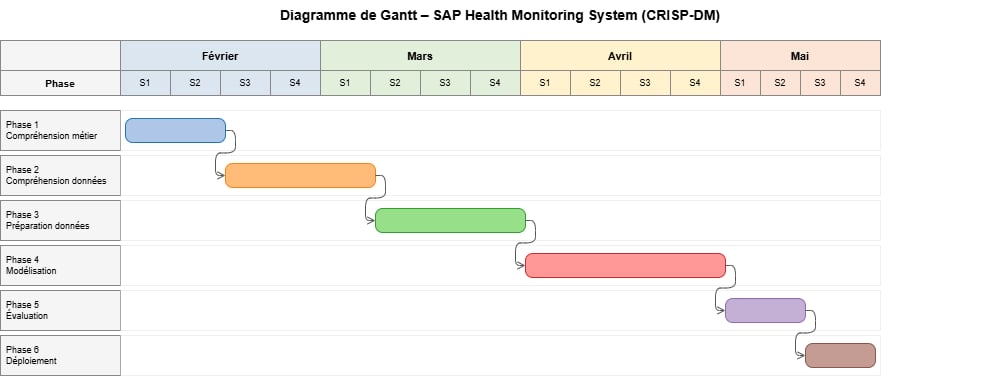
\includegraphics[width=\textwidth]{images/diagramme-de-gant.jpeg}
    \caption{Diagramme de Gantt }
    \label{fig:gantt}
\end{figure}

\section*{Conclusion}
\addcontentsline{toc}{section}{Conclusion}

Ce chapitre a posé l'ensemble des fondements du projet selon la phase Business Understanding de CRISP-DM~: contexte métier SAP et rôle du consultant BASIS, vision et objectifs de la solution, acteurs et besoins fonctionnels et non fonctionnels chiffrés, état de l'art des architectures d'IA générative (Fine-Tuning, RAG, CAG), choix d'une approche RAG hybride enrichie par cache, et planification temporelle du projet selon les six phases CRISP-DM. Le chapitre suivant aborde la phase Data Understanding en présentant les sources documentaires SAP et leur qualité.

% ============================================================
%  Chapitre 3 : Compréhension métier
% ============================================================

\chapter{Compréhension métier}
\label{chap:business_understanding}

% ============================================================
\section*{Introduction}
\addcontentsline{toc}{section}{Introduction}

Ce chapitre présente le contexte métier et les objectifs du projet de détection
d'anomalies dans le cadre de la méthodologie CRISP-DM. Il met en évidence l'importance
d'aligner les efforts techniques sur les objectifs métier, afin que la solution développée
réponde aux défis réels auxquels sont confrontées les équipes SAP.

% ============================================================
\section{État de l'art}
\label{sec:etat_art}

\subsection{Qu'est-ce qu'un ERP ?}

Un système ERP (\textit{Enterprise Resource Planning}) est un logiciel qui intègre et
gère les principaux processus métier d'une organisation : finances, ressources humaines,
fabrication, chaîne d'approvisionnement, ventes et achats. Il fournit une source unique
de vérité, élimine la duplication des données et améliore l'efficacité opérationnelle.
Les solutions ERP permettent aux entreprises d'obtenir une visibilité en temps réel sur
leurs opérations, d'automatiser les processus et de prendre des décisions basées sur
les données.

\textbf{SAP} (\textit{Systems, Applications and Products in Data Processing}) est l'un
des principaux fournisseurs de logiciels ERP. Sa suite logicielle couvre de nombreux
domaines fonctionnels. Parmi ses modules les plus utilisés :

\begin{itemize}[leftmargin=*, label=\textbullet]
  \item \textbf{SAP EWM (\textit{Extended Warehouse Management}) :} Module spécialisé
        dans l'optimisation des entrepôts et la gestion des stocks. Il aide les entreprises
        à gérer efficacement leurs opérations d'entreposage et à garantir la disponibilité
        des produits au bon moment.
  \item \textbf{SAP ECC (\textit{Enterprise Central Component}) :} Module central de
        l'ERP SAP. Il intègre les finances, les ventes, les achats, la fabrication et
        les ressources humaines au sein d'une plateforme unifiée.
  \item \textbf{SAP Solution Manager (SOLMAN) :} Outil central de gestion et de
        surveillance fourni par SAP. Il couvre la gestion du cycle de vie des applications,
        la gestion de projets, la gestion des services IT et le suivi des processus métier.
\end{itemize}

% ============================================================
\subsection{Le consultant SAP BASIS}

Le consultant SAP BASIS est responsable de l'infrastructure technique de l'environnement
SAP : installations, mises à jour et application des correctifs. Il assure la résolution
des problèmes de connectivité, les ajustements de composants et l'assistance aux systèmes
externes et aux bases de données. Ses principales responsabilités comprennent :

\begin{enumerate}[leftmargin=*, label=\arabic*.]
  \item Administration des systèmes
  \item Surveillance et optimisation des performances
  \item Administration de la sécurité
  \item Administration des bases de données
  \item Résolution des incidents techniques
  \item Sauvegarde et récupération des données
  \item Gestion des intégrations et des interfaces
  \item Mises à jour et migrations des systèmes
  \item Documentation et formation
\end{enumerate}

% ============================================================
\subsection{Les codes de transaction SAP (T-codes)}

Dans SAP, les codes de transaction (T-codes) sont des commandes alphanumériques courtes
permettant d'accéder rapidement à des fonctions spécifiques, des rapports ou des
diagnostics système. Ils servent de points d'entrée dans les modules fonctionnels de SAP,
permettant aux utilisateurs de contourner les menus profonds et d'exécuter directement
des tâches telles que la surveillance des jobs, la gestion des files d'attente ou
l'analyse des performances.

Chaque T-code correspond à une fonction ou un programme backend — généralement implémenté
en ABAP — qui effectue un ensemble défini d'opérations. Lors de l'exécution d'un T-code,
SAP vérifie les autorisations de l'utilisateur, exécute la logique associée et présente
une interface interactive.

Dans le cadre de ce projet, un ensemble de T-codes à haute criticité a été sélectionné
pour assurer une couverture complète du comportement des systèmes SAP :

\begin{itemize}[leftmargin=*, label=\textbullet]
  \item \texttt{ST22} – Analyse des erreurs d'exécution ABAP (\textit{short dumps}).
  \item \texttt{DB02} – Surveillance des statistiques de base de données (croissance,
        espace table, index manquants).
  \item \texttt{SM37} – Surveillance des jobs en arrière-plan.
  \item \texttt{SP01} – Vérification des requêtes d'impression et de leurs statuts.
  \item \texttt{SM66} – Vue globale des processus de travail actifs.
  \item \texttt{SM58} – Analyse des erreurs RFC transactionnelles (traitement asynchrone).
  \item \texttt{SMQ1}, \texttt{SMQ2} – Surveillance des files d'attente entrantes et
        sortantes (qRFC/tRFC).
  \item \texttt{SM12}, \texttt{SM13} – Révision des entrées verrouillées et des
        enregistrements de mise à jour.
  \item \texttt{ST03N} – Analyse des statistiques de charge de travail et de performance.
  \item \texttt{SOST} – Surveillance des messages SAPconnect (e-mails, fax, etc.).
  \item \texttt{ST13} – Outils BASIS pour les diagnostics approfondis et les journaux.
\end{itemize}

Ces T-codes ont été sélectionnés en raison de leur criticité pour les opérations en temps
réel, de leur pertinence pour les équipes BASIS et de leur fréquence d'utilisation lors
de la résolution des incidents. En surveillant en continu ces transactions et en
interprétant leurs sorties par le biais d'un raisonnement assisté par IA, le système
permet une détection précoce des anomalies et soutient une analyse plus rapide des causes
profondes.

% ---- SM37 ----
\subsubsection*{SM37 — Job Overview}

SM37 surveille les \textit{jobs batch} — ce sont des tâches automatiques qui
tournent en arrière-plan (traitements de données, interfaces, rapports).
L'administrateur vérifie qu'aucun job n'est en erreur ou bloqué.

\begin{figure}[H]
  \centering
  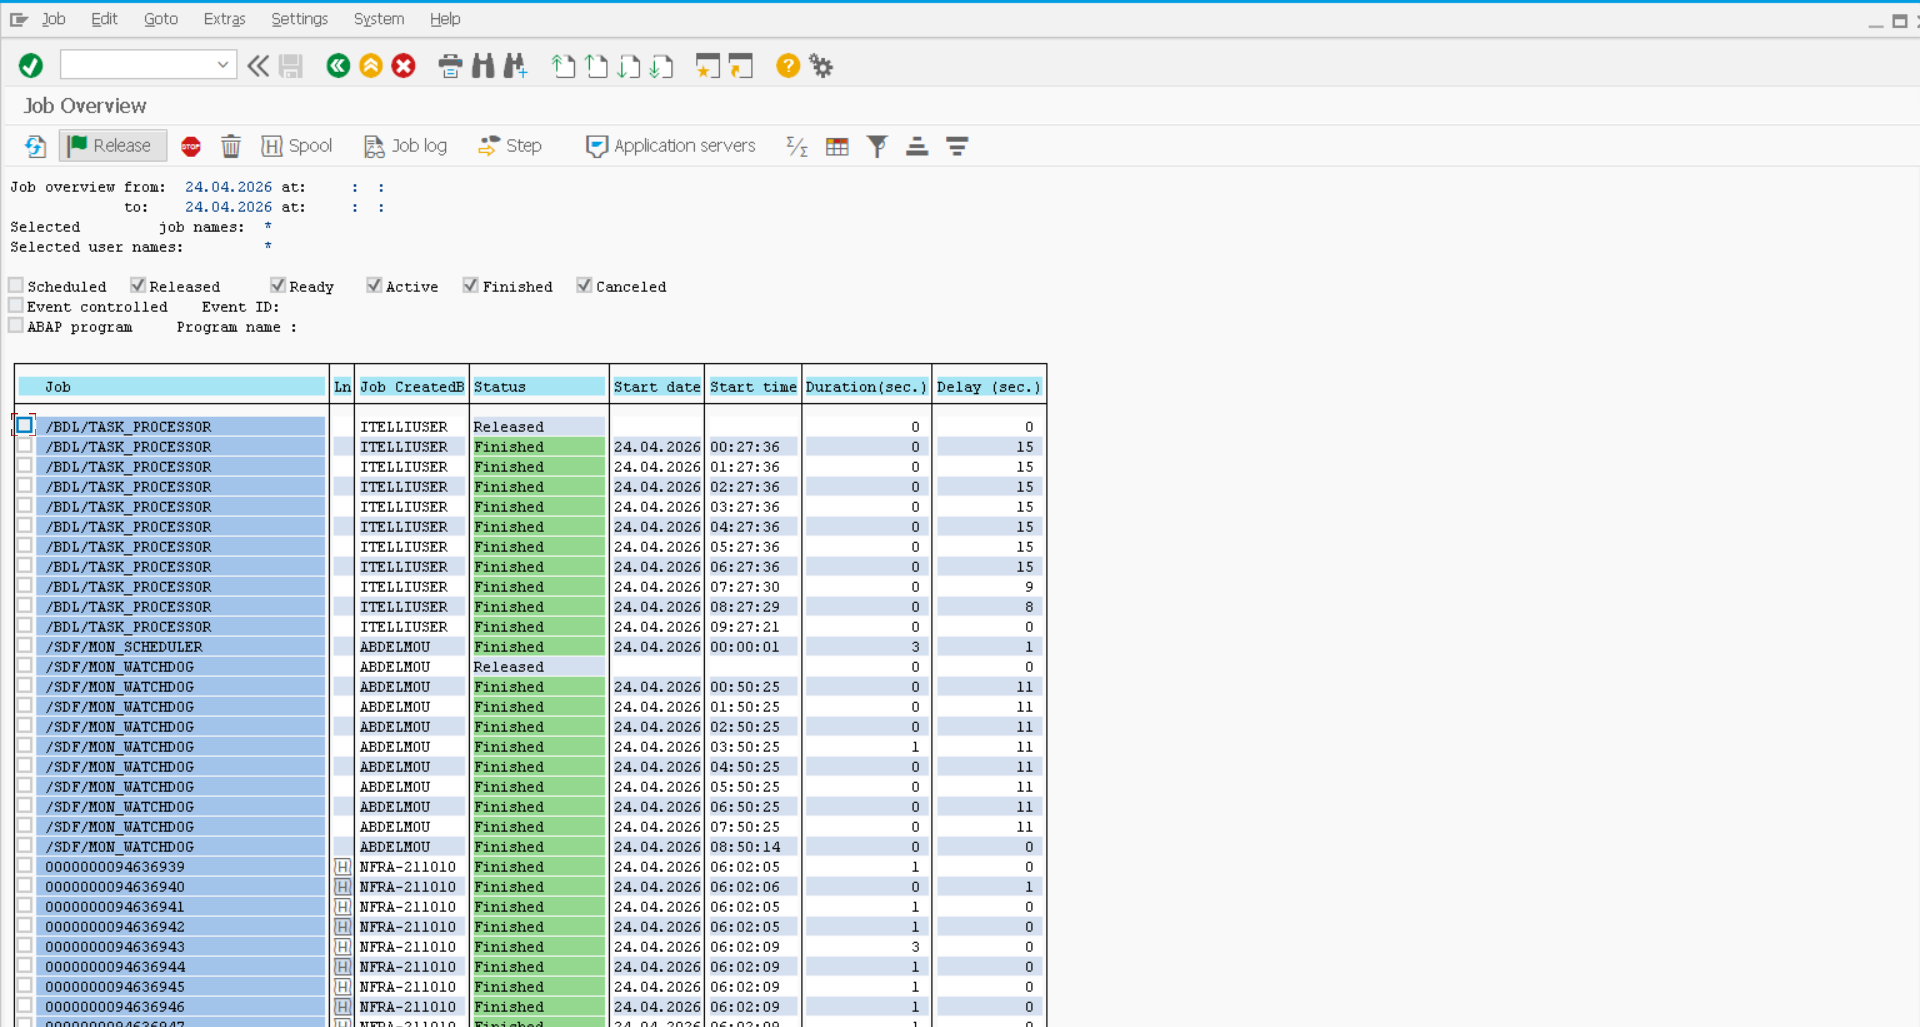
\includegraphics[width=\textwidth]{images/sm37.png}
  \caption{SM37 — Vue d'ensemble des jobs batch}
  \label{fig:sm37}
\end{figure}

La figure SM37 présente l'interface du T-code \texttt{SM37}, qui affiche
la liste des jobs planifiés avec leur statut (\textit{Finished}, \textit{Released},
\textit{Active}), leur date et heure de démarrage, leur durée d'exécution ainsi que
le délai éventuel. Cette vue permet à l'administrateur BASIS d'identifier en un coup
d'œil tout job bloqué, annulé ou présentant un délai anormal, et d'intervenir
rapidement avant que cela n'impacte les processus métier.

% ---- DB02 ----
\subsubsection*{DB02 — Space Overview}

DB02 surveille la base de données — l'administrateur contrôle l'espace disque
disponible pour éviter que la base de données sature, ce qui provoquerait un
arrêt complet du système.

\begin{figure}[H]
  \centering
  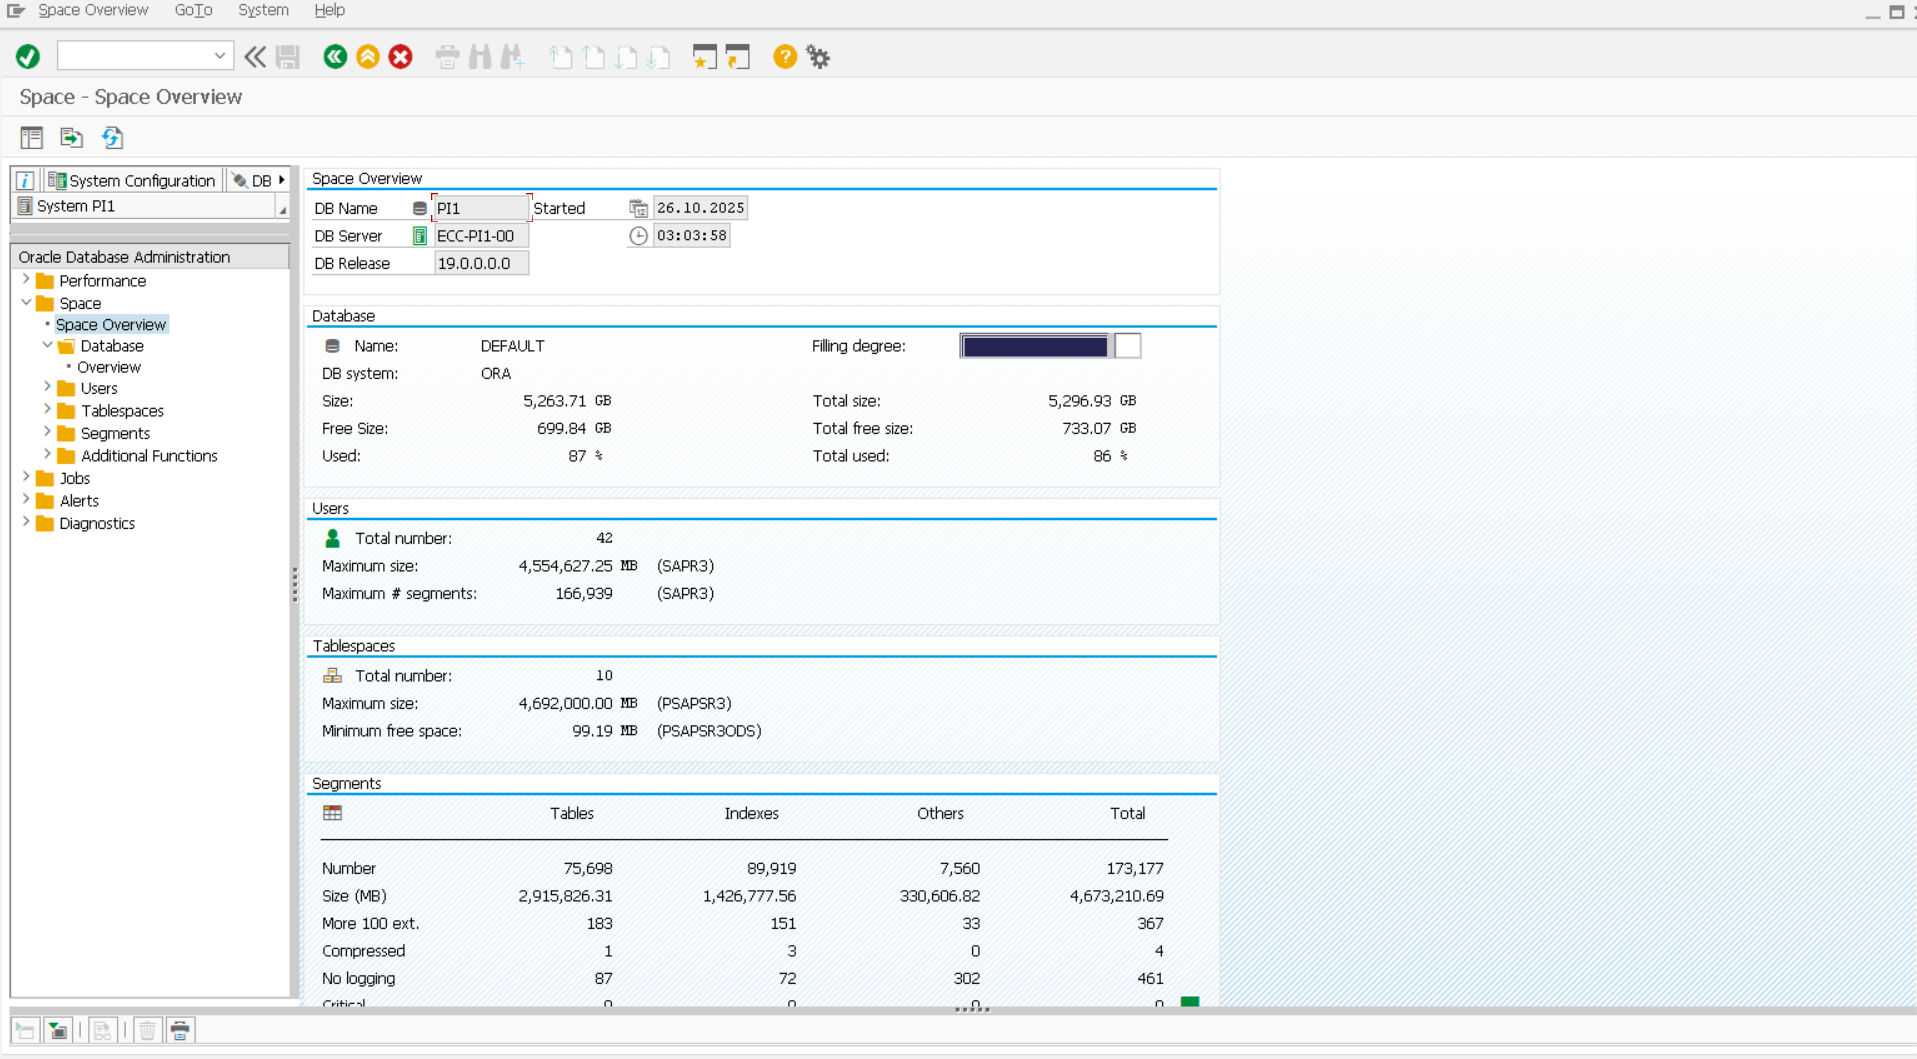
\includegraphics[width=\textwidth]{images/db02.png}
  \caption{DB02 — Vue d'ensemble de l'espace base de données}
  \label{fig:db02}
\end{figure}

La figure db02 illustre le T-code \texttt{DB02}, qui fournit une vue
synthétique de l'état de la base de données Oracle. On y retrouve le taux de
remplissage global, la taille totale et l'espace libre, ainsi que le détail par
tablespace et par segment (tables, index, autres). Un taux d'utilisation élevé —
comme les 87\% visibles ici — constitue un signal d'alerte critique nécessitant
une action immédiate d'extension ou de purge pour prévenir toute saturation du système.

% ---- ST22 ----
\subsubsection*{ST22 — Runtime Errors}

ST22 liste les erreurs critiques ABAP — l'administrateur analyse les
\textit{dumps} pour identifier les programmes qui plantent et corriger
les problèmes avant qu'ils n'impactent les utilisateurs.

\begin{figure}[H]
  \centering
  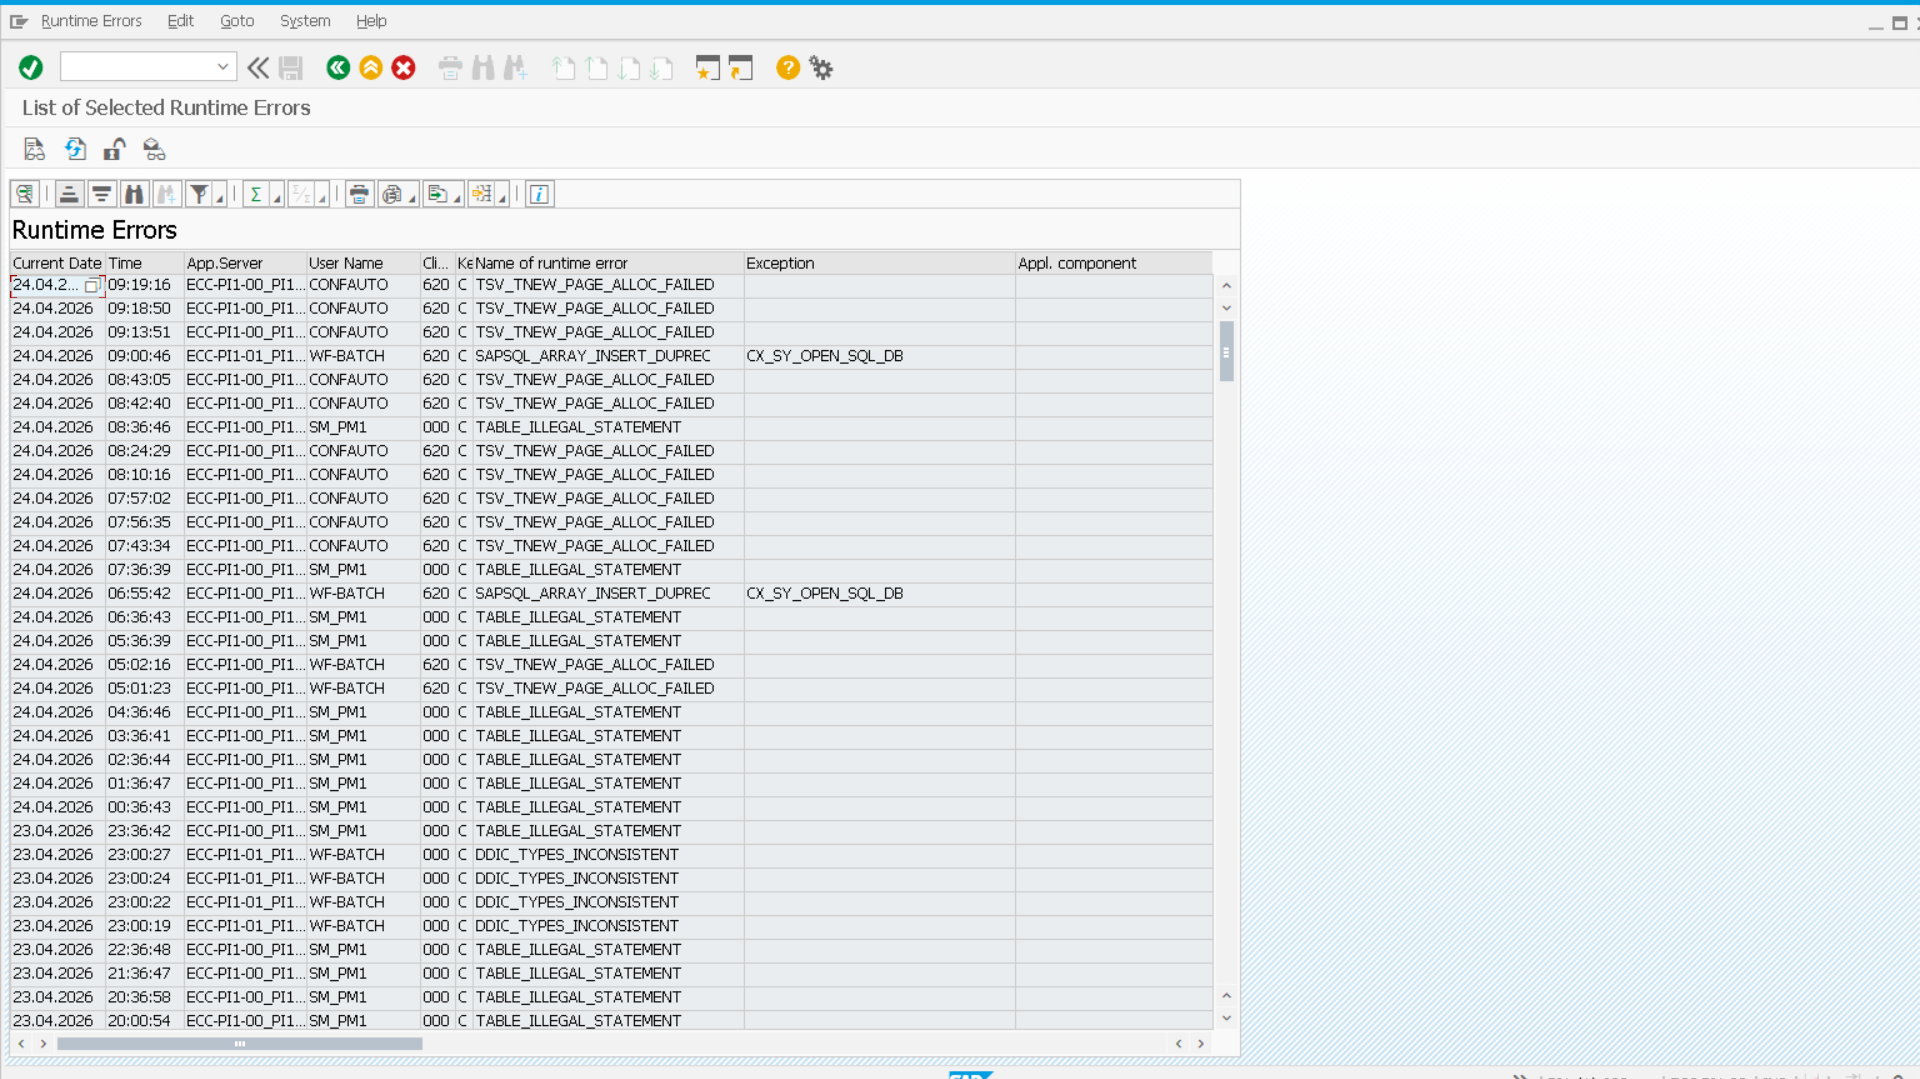
\includegraphics[width=\textwidth]{images/st22.png}
  \caption{ST22 — Liste des erreurs d'exécution ABAP}
  \label{fig:st22}
\end{figure}

La figure ST22 présente l'interface du T-code \texttt{ST22}, qui recense
l'ensemble des \textit{short dumps} ABAP survenus sur le système. Chaque entrée
indique la date, l'heure, le serveur applicatif, l'utilisateur concerné et le nom
de l'erreur. Les erreurs récurrentes telles que \texttt{TSV\_TNEW\_PAGE\_ALLOC\_FAILED}
(manque de mémoire) ou \texttt{TABLE\_ILLEGAL\_STATEMENT} (instruction SQL non autorisée)
sont des indicateurs d'anomalies systémiques qui doivent être analysées et résolues
en priorité par l'équipe BASIS.

% ============================================================
\subsection{Les Fondements Technologiques de l'IA Générative}

L'intelligence artificielle générative s'appuie sur une série de composants technologiques
complémentaires qui, lorsqu'ils sont assemblés, permettent la création de systèmes capables
d'interpréter, de raisonner et de produire du contenu à partir de données complexes. Ce
rapport se concentre sur deux éléments essentiels : les modèles de langage de grande taille
(LLMs), qui assurent la compréhension et la génération, et l'architecture RAG
(\textit{Retrieval-Augmented Generation}), qui améliore ces modèles en leur offrant une
base de savoir actualisée et vérifiable.

% ============================================================
\subsection{Architecture de l'IA RAG}

Un grand modèle de langage (LLM) détient une compréhension générale acquise lors de son
entraînement, mais il n'a pas d'accès direct à vos documents internes, à vos bases de
données confidentielles ou aux informations les plus récentes. L'architecture RAG
(\textit{Retrieval-Augmented Generation}) pallie cette lacune : avant de générer une
réponse, le système découpe d'abord les documents sources en fragments appelés
\textit{chunks} — de courts passages de quelques phrases ou paragraphes —, puis transforme
chacun d'eux en un \textit{embedding}, c'est-à-dire un vecteur numérique qui encode le
sens du texte plutôt que ses mots exacts. Ces vecteurs sont stockés dans une base de
données vectorielle, qui permet de retrouver en quelques millisecondes les chunks
sémantiquement les plus proches d'une question donnée, grâce à une mesure de similarité
cosinus. On peut percevoir le RAG comme un assistant disposant de sa propre bibliothèque :
au lieu de répondre directement de mémoire, il consulte d'abord les bonnes références,
extrait les passages essentiels, les injecte dans son contexte, puis construit une réponse
ancrée sur des faits vérifiables et traçables.
\begin{figure}[H]
  \centering
  \resizebox{\textwidth}{!}{%
  \begin{tikzpicture}[
      node distance=0.8cm and 1.5cm,
      box/.style={
          draw,
          rounded corners=8pt,
          minimum width=3cm,
          minimum height=1cm,
          align=center,
          font=\normalsize\bfseries,
          line width=1.2pt
      },
      arrow/.style={-Latex, line width=1.5pt},
      label/.style={font=\small, midway}
  ]

  % ══════════════════════════════
  % LIGNE 1 (haut) : Indexation
  % ══════════════════════════════
  \node[box, fill=yellow!40, draw=yellow!80!black] (docs)
      {Documents};

  \node[box, fill=blue!25, draw=blue!70, right=2cm of docs] (chunking)
      {Chunking};

  \node[box, fill=purple!25, draw=purple!70, right=2cm of chunking] (embedding)
      {Embeddings};

  \node[box, fill=green!30, draw=green!70, right=2cm of embedding] (vector)
      {Vector DB};

  % ══════════════════════════════
  % LIGNE 2 (bas) : Génération
  % ══════════════════════════════
  \node[box, fill=red!20, draw=red!70, below=2.5cm of vector] (retrieval)
      {Top-K \\ Retrieval};

  \node[box, fill=orange!30, draw=orange!80, left=2cm of retrieval] (llm)
      {LLM};

  \node[box, fill=cyan!25, draw=cyan!70, left=2cm of llm] (response)
      {Response};

  % ══════════════════════════════
  % USER QUERY : centré verticalement
  % ══════════════════════════════
  \node[box, fill=gray!20, draw=gray!60,
        below=2.5cm of embedding] (query)
      {User Query};

  % ══════════════════════════════
  % FLÈCHES — Indexation (ligne 1)
  % ══════════════════════════════
  \draw[arrow, blue!80]
      (docs) -- node[label, above]{\small découpage} (chunking);

  \draw[arrow, purple!80]
      (chunking) -- node[label, above]{\small vectorisation} (embedding);

  \draw[arrow, green!80]
      (embedding) -- node[label, above]{\small stockage} (vector);

  % ══════════════════════════════
  % FLÈCHES — Génération (ligne 2)
  % ══════════════════════════════
  \draw[arrow, red!80]
      (vector) -- node[label, right]{\small similarité} (retrieval);

  \draw[arrow, orange!80]
      (retrieval) -- node[label, below]{\small contexte} (llm);

  \draw[arrow, cyan!80]
      (llm) -- node[label, below]{\small génération} (response);

  % ══════════════════════════════
  % FLÈCHES — User Query
  % ══════════════════════════════
  \draw[arrow, dashed, gray!70]
      (query) -- node[label, right]{\small recherche} (vector);

  \draw[arrow, gray!70]
      (query) -- node[label, right]{\small prompt} (llm);

  \end{tikzpicture}%
  }

  \caption{Pipeline RAG : indexation, vectorisation, récupération et génération}
  \label{fig:rag_pipeline}
\end{figure}

% ============================================================
\subsection{Large Language Models (LLMs)}

Un LLM (\textit{Large Language Model}) est un type de modèle d'intelligence artificielle
qui a été formé sur d'énormes volumes de textes — tels que livres, articles, sites
internet, code — dans le but de comprendre les structures, les significations et les
connexions entre les mots d'une langue. En pratique, il anticipe le terme (ou jeton) le
plus susceptible de suivre un certain texte et c'est en répétant ce processus des milliers
de fois qu'il produit des réponses cohérentes, rédige des documents, fait des traductions,
résume ou répond à des interrogations. Plus le modèle est vaste (comportant des milliards
de paramètres), plus il a la capacité de saisir les subtilités complexes du langage. Des
exemples de LLM accessibles au public comprennent ChatGPT, Claude et Gemini.

% ============================================================
\section*{Conclusion}
\addcontentsline{toc}{section}{Conclusion}

Ce chapitre souligne l'importance stratégique du développement d'un système de détection
d'anomalies adapté aux transactions SAP dans le cadre de la méthodologie CRISP-DM. En
alignant les capacités techniques sur les objectifs métier, ce projet vise à améliorer
l'efficacité opérationnelle des équipes BASIS, à optimiser les processus de prise de
décision et à réduire le temps moyen de résolution des incidents.
\chapter{Compréhension des Données}

Ce chapitre correspond à la phase de compréhension des données du cycle CRISP-DM. Elle couvre quatre tâches : la collecte des données, leur description structurelle, leur exploration statistique et la vérification de leur qualité. Le projet mobilise deux corpus distincts : des données de surveillance opérationnelle SAP extraites en temps réel et stockées dans MongoDB, et une base de connaissances documentaire construite à partir de 297 livres de formation SAP et du portail d'aide en ligne, indexée dans PostgreSQL avec pgvector.

% ─────────────────────────────────────────────────────────────────────────────
\section{Collecte des Données}
% ─────────────────────────────────────────────────────────────────────────────

\subsection{Données de Surveillance SAP — Extraction via PyRFC}

Les données de surveillance opérationnelle sont extraites automatiquement des systèmes SAP de production par la couche \textbf{PyRFC}, le connecteur Python pour les Remote Function Calls SAP. PyRFC permet d'appeler directement les modules de fonction SAP depuis Python sans passer par la SAP GUI, rendant l'extraction répétable, planifiable et traçable.

Chaque extraction produit des enregistrements horodatés portant un champ \texttt{SID} qui identifie le système SAP source et un champ \texttt{Extraction\_Timestamp} qui permet l'historisation. Dix-huit transactions SAP sont couvertes : journaux d'erreurs ABAP (ST22), statuts de jobs (SM37), espace base de données (DB02), entrées de verrouillage (SM12), processus de travail (SM50, SM66), files qRFC (SMQ1, SMQ2), messagerie (SOST), ainsi que les métriques système CPU, mémoire et système de fichiers.

\subsection{Base de Connaissances RAG — Extraction Multi-Agent}

La base de connaissances du chatbot est construite à partir de deux sous-sources documentaires.

La première est constituée de \textbf{297 supports de cours SAP au format PDF} : administration Basis (ADM100, ADM505), développement ABAP (BC100, BC400), modules fonctionnels MM, SD, FI, et formations spécialisées NetWeaver, HANA, Fiori, sécurité. Ces documents issus du programme de formation accrédité SAP constituent la référence pédagogique la plus complète pour un technicien SAP.

La seconde est le \textbf{portail d'aide en ligne SAP} (help.sap.com), dont des sections thématiques ont été extraites par web scraping. Ce portail fournit une documentation orientée configuration, codes d'erreur, paramètres système et notes de correction (SAP Notes), complémentaire aux livres de formation.

\paragraph{Extraction PDF par agents parallèles.}
Le script \texttt{Sap\_batch\_extractor.py} orchestre un ensemble d'agents d'extraction, chacun responsable d'un sous-ensemble de livres. Chaque agent opère de façon autonome : il charge le PDF avec \textbf{pdfplumber}, détecte la hiérarchie des sections à partir de la taille et de la graisse de police, extrait le texte de chaque section, isole les figures et produit un fichier \texttt{structured\_content.json}. Le traitement en parallèle réduit le temps total d'extraction de plusieurs heures à quelques dizaines de minutes.

\paragraph{Web scraping du portail SAP.}
L'extraction des pages d'aide utilise une chaîne de trois outils : \textbf{Scrapy} pour la navigation et le téléchargement des pages statiques, \textbf{Playwright} pour les composants dynamiques chargés en JavaScript, et \textbf{BeautifulSoup} pour le parsing et le nettoyage du HTML brut.

\paragraph{Résilience SSL lors de l'ingestion.}
L'ingestion des vecteurs dans la base PostgreSQL distante hébergée sur Supabase expose le pipeline à des interruptions de connexion SSL sur des sessions de longue durée. Deux mécanismes ont été implémentés : des TCP keepalives (\texttt{keepalives\_idle=30\,s, keepalives\_interval=10\,s}) pour maintenir la connexion active, et une boucle de retry automatique en cas de drop SSL.

\begin{lstlisting}[language=Python, caption={Boucle de retry SSL dans ingest\_to\_db.py}]
for attempt in range(3):
    try:
        conn = psycopg2.connect(
            DB_URL, keepalives=1,
            keepalives_idle=30, keepalives_interval=10
        )
        # ingestion du batch
        break
    except Exception as exc:
        if "SSL" in str(exc):
            print(f"[WARN] SSL drop, retry {attempt+1}/3")
            time.sleep(2)
        else:
            raise
\end{lstlisting}

% ─────────────────────────────────────────────────────────────────────────────
\section{Description des Données}
% ─────────────────────────────────────────────────────────────────────────────

\subsection{Collections MongoDB — Données de Surveillance}

Les données de surveillance sont réparties dans dix-huit collections MongoDB, chacune correspondant à une transaction SAP ou à une métrique système. Le tableau suivant présente les collections et leurs champs principaux.

\begin{longtable}{|p{2.4cm}|p{4.0cm}|p{7.2cm}|}
\caption{Collections MongoDB et champs principaux}
\label{tab:mongo-collections}\\
\hline
\textbf{Collection} & \textbf{Transaction SAP} & \textbf{Champs principaux} \\
\hline
\endfirsthead
\hline
\textbf{Collection} & \textbf{Transaction SAP} & \textbf{Champs principaux} \\
\hline
\endhead
\texttt{ST22}      & Erreurs d'exécution ABAP     & Current\_Date, Runtime\_Error\_Name, Application\_Server, User\_Name \\
\hline
\texttt{SM37}      & Jobs en arrière-plan          & Job, Status, Start\_Date, End\_Date, Job\_Created\_By \\
\hline
\texttt{DB02}      & Espace base de données        & TableSpace\_Name, Used\_Percent, Free\_MB, AutoExtend \\
\hline
\texttt{SM12}      & Entrées de verrouillage       & Table\_Name, User\_name, Date, Time \\
\hline
\texttt{SM51}      & Serveurs d'application        & HOST, STATE \\
\hline
\texttt{SM66}      & Processus de travail          & WP\_Type, Total, Running, WP\_Ratio \\
\hline
\texttt{SM58}      & RFC transactionnel             & Function\_Module, Target\_System, Status \\
\hline
\texttt{SM13}      & Enregistrements de mise à jour & User, TCode, Status \\
\hline
\texttt{SP01}      & Demandes de spool              & Spool\_No, User\_Name, Status \\
\hline
\texttt{ST13}      & Chaînes de processus           & Chain\_ID, Log\_ID, Status \\
\hline
\texttt{ST03N}     & Analyse de charge              & Task\_Type, Average\_Response\_Time\_per\_Step \\
\hline
\texttt{SMQ1/SMQ2} & Files qRFC                    & Queue\_Name, Destination, Status \\
\hline
\texttt{SOST}      & Messagerie sortante            & Creator, ErrorMsg \\
\hline
\texttt{CPU}       & Métriques processeur           & user\_cpu\_percent, system\_cpu\_percent, idle\_cpu\_percent \\
\hline
\texttt{MEMORY}    & Métriques mémoire              & MIN\_FR\_MEM, MAX\_FR\_MEM, AVG\_SWAPFR \\
\hline
\texttt{FSYS}      & Système de fichiers            & filesystem\_path, capacity\_gb, free\_gb \\
\hline
\texttt{MSS\_DB}   & Base SQL Server                & DB\_SIZE, LOG\_SIZE, RESERVED \\
\hline
\end{longtable}

Chaque enregistrement porte également les champs transversaux \texttt{SID} (identifiant du système SAP source) et \texttt{Extraction\_Timestamp} (horodatage de l'extraction), qui permettent de surveiller plusieurs instances SAP dans la même base et de reconstituer un historique.

Le schéma de chaque document est flexible (BSON sans contrainte de colonne), ce qui permet d'adapter la structure aux spécificités de chaque transaction sans migration de schéma. Les exemples suivants illustrent la structure réelle des enregistrements.

\begin{lstlisting}[caption={Enregistrement ST22 — erreur d'exécution ABAP}]
{
  "Current_Date"       : "2024-12-11",
  "Time"               : "14:46:45",
  "Application_Server" : "ECC-SYS-00",
  "User_Name"          : "USER____",
  "Client"             : "620",
  "Runtime_Error_Name" : "DBIF_RSQL_INVALID_REQUEST",
  "SID"                : "ECC",
  "Extraction_Timestamp": "2024-12-12 11:49:32"
}
\end{lstlisting}

\begin{lstlisting}[caption={Enregistrement SM37 — job annulé}]
{
  "Job"            : "Z3_WM_UPDATE",
  "Job_Created_By" : "BATCH_USER",
  "Status"         : "Cancelled",
  "Start_Date"     : "2025-04-24",
  "Start_Time"     : "19:08:01",
  "End_Date"       : "2025-04-24",
  "End_Time"       : "19:08:01",
  "SID"            : "ECC",
  "Extraction_Timestamp": "2025-04-25 10:59:14"
}
\end{lstlisting}

\subsection{Fichiers Produits par le Pipeline RAG}

L'extraction et la transformation des données documentaires produisent une famille de fichiers intermédiaires et finaux.

\begin{table}[H]
\centering
\caption{Fichiers produits par le pipeline de traitement documentaire}
\label{tab:fichiers}
\begin{tabularx}{\textwidth}{|p{5.8cm}|X|}
\hline
\textbf{Fichier} & \textbf{Contenu} \\
\hline
\texttt{output/<COURS>/structured\_content.json} & Contenu hiérarchique extrait par livre (sections, procédures, tableaux, métadonnées) \\
\hline
\texttt{normalized/unified\_content.json} & Documents normalisés issus de toutes les sources, après nettoyage et unification du schéma \\
\hline
\texttt{chunked\_for\_embedding.json} & Segments finaux après découpage hiérarchique (parents + enfants + singles) \\
\hline
\texttt{metadata.json} & Métadonnées des 76\,463 chunks filtrés, alignées par index avec les vecteurs \\
\hline
\texttt{embeddings.npy} & Vecteurs d'embeddings — forme (76\,463, 1\,024), float32 \\
\hline
\end{tabularx}
\end{table}

\subsection{Schéma de la Table PostgreSQL \texttt{sap\_chunks}}

Tous les segments documentaires sont stockés dans une table PostgreSQL dont le schéma supporte simultanément la recherche sémantique par vecteur, le filtrage par métadonnées et la recherche plein texte BM25.

\begin{lstlisting}[language=SQL, caption={Schéma de la table sap\_chunks}]
CREATE TABLE sap_chunks (
    chunk_id            UUID PRIMARY KEY,
    text                TEXT NOT NULL,
    title               TEXT,
    source_type         VARCHAR,     -- 'technical_book' | 'sap_help'
    source_book         TEXT,
    module              VARCHAR,     -- BASIS | ABAP | MM | SD | FI | SECURITY | HANA | FIORI
    section_type        VARCHAR,     -- 'section' | 'procedure' | 'note' | 'table'
    breadcrumb          TEXT[],      -- chemin hierarchique de la section
    mentioned_tcodes    TEXT[],      -- T-codes detectes (SM37, ST22, SE38...)
    mentioned_sap_notes TEXT[],      -- numeros de notes SAP (5 a 7 chiffres)
    is_parent           BOOLEAN,     -- TRUE si chunk parent (non indexe)
    parent_chunk_id     UUID,        -- reference au chunk parent
    text_search         TSVECTOR,    -- colonne pour la recherche full-text BM25
    embedding           vector(1024) -- vecteur BGE-large-en-v1.5
);

-- Index de recherche vectorielle approximative :
CREATE INDEX sap_chunks_hnsw ON sap_chunks
    USING hnsw (embedding vector_cosine_ops)
    WITH (m = 16, ef_construction = 64);

-- Index full-text BM25 :
CREATE INDEX sap_chunks_fts ON sap_chunks USING gin(text_search);

-- Index sur les T-codes pour le filtrage par transaction :
CREATE INDEX sap_chunks_tcodes ON sap_chunks USING gin(mentioned_tcodes);
\end{lstlisting}

L'index HNSW (\textit{Hierarchical Navigable Small World}) transforme la recherche par similarité cosinus d'une complexité linéaire $O(N)$ en une complexité approximative $O(\log N)$, ce qui rend le système viable à l'échelle de 76\,463 vecteurs de 1\,024 dimensions. Les paramètres \texttt{m=16} et \texttt{ef\_construction=64} équilibrent précision de rappel et temps de construction. L'index HNSW occupe 154\,Mo, l'index GIN sur les T-codes 11\,Mo.

% ─────────────────────────────────────────────────────────────────────────────
\section{Exploration des Données}
% ─────────────────────────────────────────────────────────────────────────────

\subsection{Corpus Documentaire RAG — Distribution Volumétrique}

Après extraction, normalisation, découpage et filtrage des chunks de figures, le corpus final compte \textbf{76\,463 segments} répartis sur deux types de sources.

\begin{table}[H]
\centering
\caption{Distribution des segments par type de source}
\label{tab:distribution-source}
\begin{tabular}{lrr}
\toprule
\textbf{Source} & \textbf{Segments} & \textbf{Part} \\
\midrule
Livres de formation (\texttt{technical\_book}) & 40\,899 & 53,5\,\% \\
Portail d'aide SAP (\texttt{sap\_help})        & 35\,564 & 46,5\,\% \\
\midrule
\textbf{Total} & \textbf{76\,463} & \textbf{100\,\%} \\
\bottomrule
\end{tabular}
\end{table}

\begin{table}[H]
\centering
\caption{Distribution des segments par module SAP}
\label{tab:distribution-module}
\begin{tabular}{lr}
\toprule
\textbf{Module SAP} & \textbf{Segments (approx.)} \\
\midrule
ABAP         & 12\,699 \\
Fiori        &  6\,263 \\
BASIS        &  4\,251 \\
HANA         &  3\,994 \\
MM / SD / FI & $\approx$ 8\,000 \\
Non classifié & $\approx$ 41\,256 \\
\bottomrule
\end{tabular}
\end{table}

\subsection{Structure du Découpage Hiérarchique}

Le pipeline de segmentation produit trois types de segments. Les \textit{singles} sont des documents courts tenant en un seul segment (73\,137 unités) ; ils sont directement indexés. Les \textit{parents} sont des sections longues conservées en version intégrale pour le contexte élargi (8\,795 unités) ; ils ne sont pas embedés mais servent de réserve lors de la génération. Les \textit{enfants} sont les fragments issus de la subdivision des sections longues (32\,194 unités) ; ils sont embedés et indexés pour la recherche. La taille moyenne d'un segment feuille (single ou enfant) est de 175 tokens.

\begin{table}[H]
\centering
\caption{Structure du corpus après segmentation hiérarchique}
\label{tab:chunking}
\begin{tabular}{lrr}
\toprule
\textbf{Type de segment} & \textbf{Quantité} & \textbf{Indexé dans pgvector} \\
\midrule
Singles (documents courts) & 73\,137 & Oui \\
Parents (sections longues) &  8\,795 & Non (contexte élargi) \\
Enfants (fragments)        & 32\,194 & Oui \\
\midrule
Total produit par le chunker & 114\,126 & --- \\
Total après filtrage figures & \textbf{76\,463} & \textbf{Oui} \\
\bottomrule
\end{tabular}
\end{table}

\subsection{Couverture des T-codes SAP}

Plus de 80 codes transaction SAP distincts sont détectés dans le corpus. Les cinq T-codes les plus fréquents sont SM37, ST22, SE38, SM21 et SM50, qui concentrent l'essentiel des occurrences. La distribution est très asymétrique : quelques transactions très documentées (monitoring Basis, développement ABAP) cumulent la majorité des mentions, tandis que la plupart des 80+ T-codes détectés n'apparaissent que dans quelques segments.

\subsection{Évaluation de la Récupération}

Une évaluation sur 18 requêtes de test couvrant quatre catégories — dépannage (5 requêtes), configuration (3), procédure (5), explication (5) — donne les métriques suivantes sur le corpus filtré :

\begin{table}[H]
\centering
\caption{Métriques de récupération sur le corpus de 76\,463 segments}
\label{tab:eval}
\begin{tabular}{llr}
\toprule
\textbf{Métrique} & \textbf{Signification} & \textbf{Score} \\
\midrule
Recall@5  & Part des segments pertinents dans les 5 premiers  & 0,5256 \\
Recall@10 & Part des segments pertinents dans les 10 premiers & 1,0000 \\
MRR       & Rang moyen du premier résultat pertinent           & 1,0000 \\
nDCG@5    & Qualité du classement dans les 5 premiers          & 0,8747 \\
nDCG@10   & Qualité du classement dans les 10 premiers         & 0,9460 \\
\bottomrule
\end{tabular}
\end{table}

La MRR de 1,0 indique qu'au moins un résultat pertinent apparaît systématiquement en première position pour chaque requête de test. Le Recall@10 de 1,0 confirme que tous les segments pertinents sont récupérés dans les dix premiers résultats. Le score nDCG@10 de 0,946 reflète une qualité de classement quasi-parfaite.

% ─────────────────────────────────────────────────────────────────────────────
\section{Vérification de la Qualité des Données}
% ─────────────────────────────────────────────────────────────────────────────

\subsection{Problèmes Détectés}

L'extraction automatique de texte depuis des PDFs techniques et le scraping de pages web exposent le pipeline à plusieurs catégories de bruit identifiées lors de l'analyse du corpus.

\paragraph{Artefacts CID (Character Identifier).}
Le format PDF stocke les glyphes de certaines polices via des identifiants internes appelés codes CID. Lorsque la police n'est pas embarquée dans le fichier, pdfplumber ne peut pas décoder ces glyphes et produit des séquences du type \texttt{(cid:123)}. Ces séquences n'ont aucune valeur sémantique et dégradent la qualité de l'embedding si elles ne sont pas supprimées.

\paragraph{Résidus HTML dans les chunks du portail SAP.}
Les pages extraites du portail SAP Help contiennent par endroits des balises HTML mal nettoyées (\texttt{<b>}, \texttt{<i>}, \texttt{\&nbsp;}, \texttt{\&amp;}). Ces résidus perturbent la tokenisation et introduisent du bruit dans les vecteurs d'embedding.

\paragraph{Faux positifs dans la détection de T-codes.}
L'heuristique de détection de T-codes par expression régulière (\texttt{[A-Z]\{2,4\}\textbackslash d\{1,3\}}) génère des faux positifs sur des abréviations comme \texttt{BC100} (numéro de cours SAP) ou des identifiants de section. Ces faux positifs créent des associations incorrectes entre un segment et un T-code inexistant.

\paragraph{Gap vocabulaire du modèle d'embedding.}
Le modèle \texttt{BAAI/bge-large-en-v1.5} est un modèle généraliste entraîné sur du texte académique et web. Il ne connaît pas nativement la signification des codes transaction SAP. Sans traitement, une requête contenant « SM37 » et un segment documentant « le moniteur de jobs en arrière-plan » ne seraient pas rapprochés par similarité cosinus, car les deux formulations sont lexicalement distantes dans l'espace vectoriel du modèle.

\paragraph{Chunks de figures.}
La version initiale du corpus comptait environ 26\,500 segments issus des légendes et descriptions de figures extraites des PDFs. Ces segments contiennent des informations très fragmentaires (légendes courtes, numéros de figure, textes alternatifs) qui dégradent la précision de la récupération en introduisant des résultats non pertinents.

\paragraph{Séquences de points issues des tables des matières.}
Les tables des matières des PDFs SAP génèrent des lignes du type \texttt{Chapitre 3 .......... 42} qui, une fois extraites, polluent les segments avec des suites de points sans valeur sémantique.

\paragraph{Doublons inter-sources.}
Certaines pages du portail d'aide SAP reproduisent des extraits de livres de formation. Sans déduplication, ces segments dupliqués introduisent un biais dans la récupération en sur-représentant certains contenus.

\subsection{Actions Appliquées}

\begin{table}[H]
\centering
\caption{Problèmes détectés et traitements appliqués}
\label{tab:qualite}
\begin{tabularx}{\textwidth}{|p{4.5cm}|X|}
\hline
\textbf{Problème} & \textbf{Traitement appliqué} \\
\hline
Artefacts CID & Filtrage par expression régulière \texttt{(cid:\textbackslash d+)} en post-extraction \\
\hline
Résidus HTML & Nettoyage strict par BeautifulSoup avec suppression des balises et décodage des entités HTML \\
\hline
Faux positifs T-codes & Application d'une liste blanche de 80+ T-codes SAP connus en post-traitement \\
\hline
Gap vocabulaire & Expansion de synonymes : description textuelle de chaque T-code concaténée au segment lors de l'indexation et à la requête lors de la recherche \\
\hline
Chunks de figures & Filtrage complet des segments dont \texttt{source\_type = 'figure'} avant l'ingestion en base \\
\hline
Séquences de points & Suppression par regex des séquences \texttt{\.{3,}} dans la phase de normalisation \\
\hline
Doublons inter-sources & Déduplication par empreinte MD5 des 300 premiers caractères, avec conservation de la copie aux métadonnées les plus riches \\
\hline
\end{tabularx}
\end{table}

\subsection{Actions Prévues}

Plusieurs améliorations restent à mettre en œuvre pour les prochaines itérations du corpus.

\begin{itemize}
    \item \textbf{Enrichissement du corpus SAP Help} : la couverture des notes de correction (SAP Notes) et des messages d'erreur ABAP sera augmentée par une collecte plus systématique des sections correspondantes du portail.
    \item \textbf{Rééquilibrage des modules} : la surreprésentation d'ABAP et Fiori par rapport aux modules FI et CO sera corrigée par l'ajout de livres dédiés lors de la prochaine campagne de collecte.
    \item \textbf{Validation humaine} : un échantillon de 500 segments représentatifs fera l'objet d'une relecture manuelle pour mesurer précisément le taux de bruit résiduel.
    \item \textbf{Modèle d'embedding domaine-spécifique} : le remplacement de \texttt{bge-large-en-v1.5} par un modèle fine-tuné sur la documentation SAP est en cours d'évaluation, en utilisant les paires requête/segment identifiées lors de la phase d'évaluation.
\end{itemize}

% ============================================================
%  Chapitre 5 — Préparation des données
% ============================================================

\chapter{Préparation des données}
\label{chap:preparation_donnees}

\section*{Objectif}
\addcontentsline{toc}{section}{Objectif}

Ce chapitre décrit les étapes de préparation des données pour le pipeline RAG. Les documents SAP collectés ont été nettoyés, structurés et transformés en embeddings pour alimenter le moteur de recherche sémantique.
% ─────────────────────────────────────────────────────────────────────────────
\section{Vue d'ensemble du pipeline de préparation}
\label{sec:vue-ensemble}
% ─────────────────────────────────────────────────────────────────────────────

Le pipeline de préparation des données se compose de cinq étapes. Il démarre avec les données brutes et se termine par l’intégration finale dans la base vectorielle. Chaque étape utilise les résultats de la précédente pour produire des données intermédiaires bien définies. Cela assure un processus de transformation structuré, traçable et reproductible.

\begin{figure}[H]
\centering
\begin{tikzpicture}[
    font=\small,
    >={Stealth[length=7pt, width=5pt]},
    endpoint/.style = {
        rectangle, rounded corners=6pt,
        minimum width=12cm, minimum height=1.3cm,
        draw, line width=1pt,
        text centered, align=center, inner sep=8pt
    },
    procstep/.style = {
        rectangle, rounded corners=6pt,
        minimum width=12cm, minimum height=1.65cm,
        draw=SAPBlue, line width=1pt, fill=SAPLightBlue,
        inner xsep=6pt, inner ysep=8pt, align=left
    },
    finalprocstep/.style = {
        rectangle, rounded corners=6pt,
        minimum width=12cm, minimum height=1.65cm,
        draw=SAPGreen, line width=1pt, fill=SAPLightGreen,
        inner xsep=6pt, inner ysep=8pt, align=left
    },
    badge/.style = {
        circle, draw=SAPBlue, line width=1.2pt,
        fill=white, text=SAPBlue,
        minimum size=1cm, font=\bfseries, inner sep=0pt
    },
    finalbadge/.style = {
        circle, draw=SAPGreen, line width=1.2pt,
        fill=white, text=SAPGreen,
        minimum size=1cm, font=\bfseries, inner sep=0pt
    },
    artifact/.style = {
        rectangle, rounded corners=3pt,
        minimum width=7.5cm, minimum height=0.7cm,
        draw=SAPGray!70, line width=0.6pt, dashed,
        fill=white, font=\footnotesize\ttfamily,
        text centered, inner sep=5pt
    },
    arrow/.style = {->, thick, line width=1pt, color=SAPGray}
]

% ===== SOURCE =====
\node[endpoint, fill=SAPLightOrange, draw=SAPOrange] (raw) {%
    \textbf{\textsc{Données brutes}} \\[1pt]
    \footnotesize JSON de scraping SAP Help\,+\,\texttt{structured\_content.json} (PDF parsés)
};

% ===== STEP 1 =====
\node[procstep, below=0.55cm of raw] (step1) {%
    \begin{tabular}{@{\hspace{1.3cm}}l@{}}
    \textbf{Nettoyage et normalisation} \\[1pt]
    \footnotesize Correction de l'encodage CID, validation des T-codes, harmonisation des champs \\[1pt]
    \footnotesize\textcolor{SAPGray}{Script : \texttt{sap\_normalizer.py}}
    \end{tabular}
};
\node[badge] at ([xshift=0.55cm]step1.west) {1};

\node[artifact, below=0.28cm of step1] (a1) {unified\_content.json};

% ===== STEP 2 =====
\node[procstep, below=0.28cm of a1] (step2) {%
    \begin{tabular}{@{\hspace{1.3cm}}l@{}}
    \textbf{Suppression des doublons et du bruit} \\[1pt]
    \footnotesize Élimination des chunks répétés, des pages QCM et du contenu non documentaire \\[1pt]
    \footnotesize\textcolor{SAPGray}{Filtres qualité multi-critères}
    \end{tabular}
};
\node[badge] at ([xshift=0.55cm]step2.west) {2};

% ===== STEP 3 =====
\node[procstep, below=0.55cm of step2] (step3) {%
    \begin{tabular}{@{\hspace{1.3cm}}l@{}}
    \textbf{Découpage des documents en chunks} \\[1pt]
    \footnotesize Segmentation sémantique avec préservation du contexte hiérarchique \\[1pt]
    \footnotesize\textcolor{SAPGray}{Script : \texttt{chunker.py}}
    \end{tabular}
};
\node[badge] at ([xshift=0.55cm]step3.west) {3};

\node[artifact, below=0.28cm of step3] (a3) {chunked\_for\_embedding.json};

% ===== STEP 4 =====
\node[procstep, below=0.28cm of a3] (step4) {%
    \begin{tabular}{@{\hspace{1.3cm}}l@{}}
    \textbf{Génération des embeddings} \\[1pt]
    \footnotesize Vectorisation dense des chunks pour la recherche sémantique \\[1pt]
    \footnotesize\textcolor{SAPGray}{Script : \texttt{embedder.py}}
    \end{tabular}
};
\node[badge] at ([xshift=0.55cm]step4.west) {4};

\node[artifact, below=0.28cm of step4] (a4) {embeddings.npy + metadata.json};

% ===== STEP 5 (final, green) =====
\node[finalprocstep, below=0.28cm of a4] (step5) {%
    \begin{tabular}{@{\hspace{1.3cm}}l@{}}
    \textbf{Ingestion en base vectorielle} \\[1pt]
    \footnotesize Insertion des vecteurs et métadonnées dans PostgreSQL\,+\,pgvector \\[1pt]
    \footnotesize\textcolor{SAPGray}{Script : \texttt{ingest\_to\_db.py}}
    \end{tabular}
};
\node[finalbadge] at ([xshift=0.55cm]step5.west) {5};

% ===== ARROWS =====
\draw[arrow] (raw)   -- (step1);
\draw[arrow] (step1) -- (a1);
\draw[arrow] (a1)    -- (step2);
\draw[arrow] (step2) -- (step3);
\draw[arrow] (step3) -- (a3);
\draw[arrow] (a3)    -- (step4);
\draw[arrow] (step4) -- (a4);
\draw[arrow] (a4)    -- (step5);
\end{tikzpicture}
\caption{Pipeline complet de préparation des données }
\end{figure}



% ─────────────────────────────────────────────────────────────────────────────
\section{Nettoyage des données}
\label{sec:nettoyage}
% ─────────────────────────────────────────────────────────────────────────────

\subsection{Problèmes identifiés dans les données brutes}

Les données collectées à partir du portail SAP Help et des fichiers PDF présentent plusieurs problèmes de qualité. Les pages web contiennent des balises HTML résiduelles, des entités HTML, des URLs intégrées dans le texte et des titres dupliqués. Les fichiers PDF, quant à eux, comportent des caractères incorrects dus à l’encodage, des symboles indésirables et du bruit provenant des tables des matières. Ces anomalies rendent les données difficiles à utiliser directement dans le pipeline RAG. Cela nécessite une phase de nettoyage préalable.

Sans traitement, ces artefacts pollueraient les embeddings et dégraderaient la qualité de
la recherche sémantique~: un vecteur calculé sur un texte contenant des centaines de codes
CID ne représente plus le sens du document, mais le bruit de l'extraction.

\subsection{Les  opérations de normalisation}

Le module \texttt{sap\_normalizer.py} applique six opérations de nettoyage sur chaque
document, dans un ordre précis. Ces opérations sont les mêmes pour les documents issus du
portail SAP et pour les livres PDF, garantissant un schéma unifié en sortie.

\begin{table}[H]
\centering
\caption{Les six opérations de normalisation appliquées à chaque document}
\label{tab:six-ops}
\begin{tabularx}{\textwidth}{@{}clXl@{}}
\toprule
\textbf{N°} & \textbf{Opération} & \textbf{Description} & \textbf{Exemple} \\
\midrule
1 & Correction encodage & Supprime les codes CID des polices PDF, corrige le mojibake Unicode & \texttt{(cid:34)} → espace \\
\addlinespace
2 & Normalisation espaces & Réduit les espaces multiples, limite les sauts de ligne à deux maximum & \texttt{"SM  37"} → \texttt{"SM37"} \\
\addlinespace
3 & Suppression HTML & Retire les balises HTML réelles, préserve les placeholders SAP comme \texttt{<HOST>} & \texttt{<br/>}, \texttt{\&nbsp;} → supprimés \\
\addlinespace
4 & Normalisation T-codes & Fusionne les codes transactionnels mal formatés & \texttt{"SM 37"} → \texttt{"SM37"} \\
\addlinespace
5 & Formatage SAP Notes & Uniformise les références aux notes SAP & \texttt{"\#2031538"} → \texttt{"SAP Note 2031538"} \\
\addlinespace
6 & Casse acronymes SAP & Corrige la capitalisation des termes techniques & \texttt{"abap"} → \texttt{"ABAP"} \\
\bottomrule
\end{tabularx}
\end{table}



\subsection{Expansion sémantique des termes SAP}
Les modèles d'embedding n'ont pas été entraînés sur de la documentation SAP et ne connaissent pas la signification des T-codes comme SM37 ou PFCG. Pour compenser ce manque, chaque document contenant des T-codes reconnus reçoit une extension textuelle à la fin. Cette extension associe chaque T-code à sa description en anglais courant.

\begin{lstlisting}[language=Python, caption={Exemple d'expansion sémantique pour SM37}]
# Texte original
"La transaction SM37 permet de surveiller les jobs en arriere-plan."

# Texte apres expansion
"La transaction SM37 permet de surveiller les jobs en arriere-plan.
[SAP context: SM37=job monitor background job overview scheduled
jobs batch processing]"
\end{lstlisting}

Cette technique permet à un utilisateur posant la question
\textit{«~comment vérifier mes jobs de nuit~?»} de retrouver les documents qui mentionnent
SM37, même si sa question ne contient pas le code lui-même.

% ─────────────────────────────────────────────────────────────────────────────
\section{Suppression des doublons et du bruit}
\label{sec:deduplication}
% ─────────────────────────────────────────────────────────────────────────────

\subsection{Stratégie de déduplication en deux passes}

Le processus de suppression des doublons se fait après la fusion des différentes sources de données pour éviter d’avoir des documents répétés dans la base de connaissances. Cette étape se déroule en deux phases.

La première phase consiste à identifier les documents web identiques en utilisant le titre et l'URL de chaque page. Cette méthode aide à repérer les pages du portail SAP qui ont été récupérées plusieurs fois lors de différentes sessions de collecte.

La seconde phase s’appuie sur l'examen du contenu des documents. Une empreinte numérique est créée à partir du texte pour repérer les contenus similaires ou totalement identiques, même s'ils viennent de sources différentes. Cette méthode aide à identifier les passages du portail SAP qui apparaissent aussi dans certains supports de formation PDF.

% --- Add to your preamble if not already present -------------------------
% \usepackage{tikz}
% \usepackage{float}
% \usetikzlibrary{shapes.geometric, arrows.meta, positioning, calc}
%
% --- If your SAP* colors aren't defined globally, add this once: ---------
% \definecolor{SAPBlue}{RGB}{0,112,166}
% \definecolor{SAPLightBlue}{RGB}{220,235,247}
% \definecolor{SAPGray}{RGB}{100,100,100}
% \definecolor{SAPLightGray}{RGB}{240,240,240}
% \definecolor{SAPGreen}{RGB}{56,138,67}
% \definecolor{SAPLightGreen}{RGB}{225,242,225}
% \definecolor{SAPRed}{RGB}{187,40,52}
% -------------------------------------------------------------------------

\begin{figure}[H]
\centering
\begin{tikzpicture}[
    >={Stealth[length=5pt]},
    every node/.style={inner sep=3pt},
    start/.style={rectangle, rounded corners=8pt, draw=SAPBlue, thick,
                  fill=SAPLightBlue, minimum width=3.8cm, minimum height=0.8cm,
                  text centered, font=\small\bfseries},
    decision/.style={diamond, draw=SAPBlue, thick, fill=SAPLightBlue,
                     text width=2.2cm, text centered, font=\footnotesize,
                     inner sep=0pt, aspect=2.2},
    action/.style={rectangle, rounded corners=3pt, draw=SAPGray, thick,
                   fill=SAPLightGray, minimum width=3.8cm, minimum height=0.8cm,
                   text centered, font=\small},
    terminal/.style={rectangle, rounded corners=8pt, draw=SAPGreen, thick,
                     fill=SAPLightGreen, minimum width=3.8cm, minimum height=0.8cm,
                     text centered, font=\small\bfseries},
    trash/.style={rectangle, rounded corners=8pt, draw=SAPRed, thick,
                  fill=red!10, minimum width=3.2cm, minimum height=0.75cm,
                  text centered, font=\footnotesize\bfseries},
    arr/.style={->, thick, color=SAPGray, line width=0.7pt},
    edgelabel/.style={font=\scriptsize\itshape, fill=white, inner sep=2pt}
]

% --- Nodes --------------------------------------------------------------
\node[start]                          (start) {Document nettoyé};
\node[decision, below=0.7cm of start] (d1)    {Source = web~?};
\node[action,   below=0.9cm of d1]    (key)   {Calcul de la clé\\(titre, URL)};
\node[decision, below=0.7cm of key]   (d2)    {Clé déjà\\rencontrée~?};
\node[trash,    right=1.6cm of d2]    (del1)  {Doublon web};
\node[action,   below=1.0cm of d2]    (md5)   {Empreinte MD5\\(500 premiers car.)};
\node[decision, below=0.7cm of md5]   (d3)    {Empreinte déjà\\rencontrée~?};
\node[trash,    right=1.6cm of d3]    (del2)  {Doublon contenu};
\node[terminal, below=0.7cm of d3]    (keep)  {Document conservé};

% --- Pass annotations ---------------------------------------------------
\node[font=\scriptsize\bfseries\itshape, text=SAPBlue, anchor=east]
      at ([xshift=-1.8cm]key.west) {Passe 1};
\node[font=\scriptsize\bfseries\itshape, text=SAPBlue, anchor=east]
      at ([xshift=-1.8cm]md5.west) {Passe 2};

% --- Flow ---------------------------------------------------------------
\draw[arr] (start) -- (d1);
\draw[arr] (d1)    -- node[edgelabel] {oui} (key);
\draw[arr] (key)   -- (d2);
\draw[arr] (d2)    -- node[edgelabel] {oui} (del1);
\draw[arr] (d2)    -- node[edgelabel] {non} (md5);

% PDF bypass: split into two segments so the label has a clear midpoint
\coordinate (bypass) at ([xshift=-1.4cm]d1.west);
\draw[arr] (d1.west) -- node[edgelabel, above] {non} (bypass);
\draw[arr] (bypass) |- (md5.west);

\draw[arr] (md5) -- (d3);
\draw[arr] (d3)  -- node[edgelabel] {oui} (del2);
\draw[arr] (d3)  -- node[edgelabel] {non} (keep);

\end{tikzpicture}
\caption[Algorithme de déduplication en deux passes]%
{Algorithme de déduplication en deux passes appliqué après l'étape de
normalisation. La première passe, restreinte aux documents issus du
\emph{scraping} web, élimine les doublons stricts identifiés par le couple
(titre, URL). La seconde passe, appliquée à l'ensemble du corpus, détecte les
contenus quasi-identiques au moyen d'une empreinte MD5 calculée sur les 500
premiers caractères, indépendamment de la source du document.}
\label{fig:dedup}
\end{figure}

\subsection{Filtrage du bruit sémantique}

Certaines documents sont techniquement valides — sans doublons et avec un texte soigné — mais ne sont pas utiles pour un système RAG de support technique. C'est notamment le cas des pages de quiz et d'auto-évaluation sur le portail SAP Help, qui contiennent des questions à choix multiples telles que \textit{«~Déterminez si cette affirmation est vraie ou fausse~»}. Ces pages nuisent à la base de connaissances, car le moteur de recherche pourrait les afficher en réponse à des requêtes légitimes, fournissant ainsi des réponses de type examen plutôt que des réponses techniques. Un filtre basé sur des expressions régulières permet d'identifier et d'éliminer ces pages en repérant des motifs tels que \texttt{learning assessment}, \texttt{determine whether this statement} ou \texttt{choose the correct answer} dans le titre ou dans les 200 premiers caractères du contenu.

\begin{table}[H]
\centering
\caption{Filtres de qualité appliqués après fusion des sources}
\label{tab:filtres}
\begin{tabularx}{\textwidth}{@{}lXl@{}}
\toprule
\textbf{Type de filtre} & \textbf{Méthode} & \textbf{Portée} \\
\midrule
Doublon exact (web) & Empreinte (titre + URL) & Documents web uniquement \\
\addlinespace
Doublon contenu & MD5 des 500 premiers caractères & Toutes sources \\
\addlinespace
Pages quiz & Regex sur titre et début de contenu & Toutes sources \\
\addlinespace
Contenu trop court & Longueur $<$ 50 caractères & Toutes sources \\
\bottomrule
\end{tabularx}
\end{table}

% ─────────────────────────────────────────────────────────────────────────────
\section{Découpage des documents (Chunking)}
\label{sec:chunking}
% ─────────────────────────────────────────────────────────────────────────────
\subsection{Qu’est-ce que le découpage }

Le découpage consiste à découper de grands ensembles de texte ou de données en segments plus petits et plus faciles à gérer, appelés « chunks ». Cette technique est utile lorsqu’on travaille avec des modèles d’apprentissage automatique qui ont des limites de taille d’entrée. Elle est également efficace pour traiter de grands volumes de données transactionnelles, où chaque entrée doit être analysée séparément tout en contribuant à des analyses globales.
\subsection{Pourquoi découper les documents~?}

LLe modèle d'embedding  peut traiter un maximum de 512 tokens en entrée. Toutefois, la documentation SAP contient souvent des textes bien plus longs que cette limite, atteignant parfois plusieurs milliers de tokens. Dans ce cas, soumettre un document complet au modèle entraînerait une troncature automatique, ce qui provoquerait une perte d'informations, en particulier dans les sections finales du document.

D'un autre côté, une segmentation simpliste ou non régulée des textes pourrait affecter la continuité sémantique des informations et réduire la qualité des représentations vectorielles générées. Il est donc nécessaire que le processus de découpage remplit deux buts : garantir que les morceaux sont compatibles avec la fenêtre de contexte du modèle et préserver la cohérence sémantique indispensable pour une représentation exacte du contenu.
\subsection{Stratégie hiérarchique parent-enfant}

L'application de la base vectorielle s'appuie sur une méthode de découpage hiérarchique qui garantit la conservation de la structure des documents tout en améliorant l'efficacité de recherche et de récupération d'information. Cette approche a été spécifiquement élaborée pour gérer la complexité et l'imbrication de la documentation SAP.

\subsubsection{Extraction sensible à la structure et au contenu}

Le système applique une méthode d'extraction basée sur la structure pour maintenir l'organisation logique et sémantique des documents SAP. Cette méthode permet de garder la hiérarchie des sections et les liens entre les divers composants du document, ce qui améliore la qualité de l'indexation et de la recherche d'informations.
\paragraph{Extraction basée sur la mise en page}

Le processus d’extraction prend en compte la structure visuelle et organisationnelle des documents à travers plusieurs mécanismes :

\begin{itemize}
\item Conservation de la hiérarchie des titres (\texttt{H1}, \texttt{H2}, \texttt{H3}, etc.) ;
\item Préservation des relations parent-enfant entre les sections et sous-sections ;
\item Identification et traitement des tableaux sous une représentation structurée de type HTML ;
\item Reconnaissance des listes et maintien de leur niveau d’imbrication.
\end{itemize}

\paragraph{Traitement enrichi par les métadonnées}

Le système extrait et conserve différentes catégories de métadonnées afin d’améliorer l’organisation documentaire et la précision de la récupération :

\begin{itemize}
\item Métadonnées générales du document (titre, date de création, version) ;
\item Métadonnées structurelles liées à l’organisation du contenu ;
\item Métadonnées techniques telles que les associations aux modules SAP ou les références aux codes de transaction.
\end{itemize}

\subsubsection{Traitement multi-niveaux du contenu}

Le contenu documentaire est analysé à plusieurs niveaux afin de capturer à la fois la structure globale du document et les caractéristiques spécifiques de chaque élément.

\paragraph{Analyse au niveau des blocs}

Cette étape comprend :

\begin{itemize}
\item La détection automatique des titres à partir de leur position, formatage et propriétés textuelles ;
\item La classification des types de contenu afin de distinguer les paragraphes, listes, tableaux et images ;
\item Une analyse spatiale exploitant les coordonnées des éléments pour reconstruire la disposition du document.
\end{itemize}

\paragraph{Traitement spécifique selon le type de contenu}

Chaque type de contenu bénéficie d’un traitement adapté :

\begin{itemize}
\item Les tableaux complexes sont convertis vers un format HTML structuré afin de préserver leur organisation ;
\item Les éléments de listes associés sont regroupés dans des fragments cohérents ;
\item Les images font l’objet d’un processus d’extraction sémantique basé sur le modèle \texttt{microsoft/Florence-2-large}. Ce choix a été retenu après une évaluation comparative avec \texttt{GLM-OCR} ainsi qu’une approche reposant uniquement sur \texttt{Tesseract OCR}. Contrairement à une simple reconnaissance optique de caractères, le modèle Florence-2-large permet de mieux préserver le contexte et la signification des informations visuelles présentes dans les schémas, captures d’écran et illustrations techniques de la documentation SAP ;
\item Les légendes et descriptions associées aux images sont reliées automatiquement au contenu visuel correspondant.
\end{itemize}



\subsection{Algorithme de découpage et chevauchement}

L'algorithme de découpage interne cherche toujours à opérer aux frontières les plus naturelles du texte. Il tente d'abord de sectionner entre les \textbf{paragraphes} (délimités par deux sauts de ligne), ensuite entre les \textbf{phrases} (séparées par «~.~», «~!~» ou «~?~»), et finalement entre les \textbf{mots} en dernier recours.

Pour éviter toute perte de contexte aux frontières entre deux fragments successifs, chaque nouveau fragment débute avec les \textbf{50 derniers tokens} du fragment précédent. Ce chevauchement (\textit{overlap}) d'environ 10\,\% assure que les phrases qui traversent une limite de découpage restent compréhensibles dans les deux fragments.
\begin{table}[H]
\centering
\caption{Niveaux de découpage par ordre de priorité}
\label{tab:niveaux-decoupage}
\begin{tabular}{@{}clll@{}}
\toprule
\textbf{Priorité} & \textbf{Niveau} & \textbf{Déclencheur} & \textbf{Séparateur} \\
\midrule
1 & Paragraphe & Paragraphe seul $>$ 512 tokens & \texttt{\textbackslash n\textbackslash n} \\
2 & Phrase & Phrase seule $>$ 512 tokens & \texttt{. ! ?} \\
3 & Mot & Phrase extrêmement longue & espace \\
\bottomrule
\end{tabular}
\end{table}

\subsection{Résultats du découpage}

Après application du chunker sur l'ensemble du corpus normalisé, les statistiques obtenues
sont les suivantes~:

\begin{table}[H]
\centering
\caption{Statistiques de découpage du corpus SAP}
\label{tab:stats-chunking}
\begin{tabular}{@{}lrp{6cm}@{}}
\toprule
\textbf{Type d'enregistrement} & \textbf{Nombre} & \textbf{Description} \\
\midrule
Singles  & 73\,137 & Documents courts — un seul enregistrement embedded \\
Parents  & 8\,795  & Documents longs — texte complet, stocké, non embedded \\
Enfants  & 32\,194 & Fragments de documents longs, embedded et indexés \\
\midrule
\textbf{Total} & \textbf{114\,126} & \textbf{Enregistrements } \\
\bottomrule
\end{tabular}
\end{table}



% ─────────────────────────────────────────────────────────────────────────────
\section{Transformation des données en embeddings vectoriels}
\label{sec:embeddings}
% ─────────────────────────────────────────────────────────────────────────────

\subsection{Choix du modèle d'embedding}

Le modèle retenu pour la génération des vecteurs est \textbf{BAAI/bge-large-en-v1.5}, un
modèle de la famille BGE (\textit{BAAI General Embedding}) publié par l'Institut de
l'Intelligence Artificielle de Pékin. Ce modèle produit des vecteurs denses de 1\,024
dimensions et a été entraîné pour la recherche sémantique dense en anglais, ce qui
correspond à la langue principale de la documentation SAP technique.

\begin{table}[H]
\centering
\caption{Comparaison des modèles d'embedding évalués}
\label{tab:modeles-embedding}
\renewcommand{\arraystretch}{1.4}
\setlength{\tabcolsep}{10pt}
\begin{tabularx}{\textwidth}{@{} l c c X X @{}}

\toprule
\rowcolor{gray!20}
\textbf{Modèle} & \textbf{Dim.} & \textbf{Langue} & \textbf{Points forts} & \textbf{Limitation} \\
\midrule

\rowcolor{blue!5}
\textbf{bge-large-en-v1.5}
  & 1\,024
  & Anglais
  & Très performant sur benchmarks BEIR
  & Monolingue \\

bge-m3
  & 1\,024
  & Multilingue
  & Supporte 100+ langues
  & Légèrement moins précis en anglais \\

\rowcolor{blue!5}
all-MiniLM-L6-v2
  & 384
  & Anglais
  & Rapide et léger
  & Moins précis \\

text-embedding-ada-002
  & 1\,536
  & Multilingue
  & API OpenAI, très utilisé
  & Payant, dépendance externe \\

\bottomrule
\end{tabularx}

\smallskip
\footnotesize\textit{Dim. = Dimensionnalité du vecteur d'embedding produit par le modèle.}
\end{table}

Le modèle bge-large-en-v1.5 a été retenu pour ses performances supérieures sur des tâches
de recherche documentaire technique, avec une fenêtre de 512 tokens alignée exactement sur
la taille maximale de nos chunks.

\subsection{Processus de génération des vecteurs}

Le script \texttt{embedder.py} prend en entrée le fichier
\texttt{chunked\_for\_embedding.json} et produit deux fichiers indexés de manière alignée~:
\texttt{embeddings.npy} (tableau NumPy de forme $(N, 1\,024)$) et \texttt{metadata.json}
(liste de $N$ dictionnaires). L'alignement par indice garantit que le vecteur
\texttt{embeddings[i]} correspond exactement au document \texttt{metadata[i]}.

Le modèle BGE requiert un préfixe spécifique ajouté à chaque texte avant l'encodage pour
signaler qu'il s'agit d'un document (et non d'une requête)~:



Les vecteurs produits sont normalisés en L2, ce qui signifie que la similarité cosinus
entre deux vecteurs est équivalente à leur produit scalaire. Cette propriété accélère
significativement la recherche dans pgvector.


% ─────────────────────────────────────────────────────────────────────────────
\section{Structuration des métadonnées}
\label{sec:metadonnees}
% ─────────────────────────────────────────────────────────────────────────────

\subsection{Rôle des métadonnées dans un système RAG}

Dans un système RAG, les métadonnées jouent un rôle aussi important que les vecteurs
eux-mêmes. Elles permettent d'appliquer des filtres \textit{avant} la recherche vectorielle,
réduisant l'espace de recherche et améliorant la précision des résultats. Par exemple, une
question portant sur la gestion des background jobs peut être filtrée sur le champ
\texttt{module = "BASIS"} avant même de comparer les vecteurs, excluant d'emblée les
documents d'autres modules SAP.

\subsection{Schéma des métadonnées}

Chaque enregistrement porte quatre catégories de métadonnées définies dans
 et transportées jusqu'en base de données .

\begin{table}[H]
\centering
\caption{Champs d'identification et de source}
\label{tab:meta-source}
\begin{tabularx}{\textwidth}{@{}llX@{}}
\toprule
\textbf{Champ} & \textbf{Type} & \textbf{Description} \\
\midrule
\texttt{doc\_id}      & string & Identifiant unique du document d'origine \\
\texttt{source\_type} & string & \texttt{"sap\_help"} ou \texttt{"technical\_book"} \\
\texttt{source\_book} & string & Nom du livre PDF source (si applicable) \\
\texttt{title}        & string & Titre de la section ou du document \\
\texttt{module}       & string & Module SAP concerné (BASIS, ABAP, FI, etc.) \\
\bottomrule
\end{tabularx}
\end{table}

\begin{table}[H]
\centering
\caption{Champs de structure hiérarchique et d'entités SAP}
\label{tab:meta-structure}
\begin{tabularx}{\textwidth}{@{}llX@{}}
\toprule
\textbf{Champ} & \textbf{Type} & \textbf{Description} \\
\midrule
\texttt{heading\_level}      & entier & Niveau de titre (H1=1, H2=2, H3=3…) \\
\texttt{section\_type}       & string & Type de section (procedure, code, note, table) \\
\texttt{breadcrumb}          & liste  & Chemin hiérarchique dans le document \\
\texttt{mentioned\_tcodes}   & liste  & T-codes cités dans le document, ex. [\texttt{"SM37"}, \texttt{"ST22"}] \\
\texttt{mentioned\_sap\_notes} & liste & Numéros de SAP Notes référencées \\
\texttt{contains\_code}      & bool   & Le document contient du code ABAP \\
\texttt{contains\_table}     & bool   & Le document contient un tableau \\
\texttt{contains\_procedure} & bool   & Le document décrit une procédure étape par étape \\
\bottomrule
\end{tabularx}
\end{table}

\begin{table}[H]
\centering
\caption{Champs de liaison parent-enfant}
\label{tab:meta-hierarchy}
\begin{tabularx}{\textwidth}{@{}llX@{}}
\toprule
\textbf{Champ} & \textbf{Type} & \textbf{Description} \\
\midrule
\texttt{is\_parent}       & bool   & \texttt{True} si enregistrement parent (non embedded) \\
\texttt{parent\_chunk\_id} & string & UUID du parent (vide si single ou parent) \\
\texttt{chunk\_index}      & entier & Position du fragment dans le document ($-1$ pour parent) \\
\texttt{chunk\_total}      & entier & Nombre total de fragments du document \\
\bottomrule
\end{tabularx}
\end{table}

\subsection{Stockage et indexation dans PostgreSQL}

Les chunks extraits sont persistés dans une base de données PostgreSQL enrichie de
l'extension \textbf{pgvector}, qui ajoute un type de données natif pour les vecteurs
denses et les opérateurs de similarité associés. L'ensemble des données est stocké dans
une table unique \texttt{sap\_chunks}, dont le schéma est défini comme suit~:

\begin{lstlisting}[language=SQL, caption={Schéma de la table \texttt{sap\_chunks}}]
CREATE TABLE sap_chunks (
    id        UUID           PRIMARY KEY,
    content   TEXT           NOT NULL,
    metadata  JSONB,
    embedding vector(1024)
);
\end{lstlisting}

Chaque enregistrement correspond à un chunk textuel identifié par un UUID, accompagné
de son contenu brut, de ses métadonnées structurées et de son vecteur d'embedding de
dimension 1\,024. La colonne \texttt{metadata} adopte le type \textbf{JSONB} (JSON
Binaire), format natif de PostgreSQL permettant des requêtes conditionnelles efficaces
sur des champs imbriqués arbitraires.

\medskip
Afin d'assurer des performances de recherche adaptées à un usage en production, deux
index complémentaires sont définis sur cette table~:

\begin{itemize}
    \item \textbf{Index HNSW} (\textit{Hierarchical Navigable Small World})~: appliqué
    sur la colonne \texttt{embedding}, cet index permet la recherche approximative des
    plus proches voisins par similarité cosinus. Il est configuré avec les paramètres
    \texttt{m=16} et \texttt{ef\_construction=64}, qui contrôlent respectivement le
    nombre de liens par nœud dans le graphe et la précision du processus de construction.

    \item \textbf{Index GIN} (\textit{Generalized Inverted Index})~: appliqué sur la
    colonne \texttt{metadata}, il accélère les filtres JSONB du type
    \texttt{metadata @> '\{"module": "BASIS"\}'}, permettant de restreindre l'espace de
    recherche vectorielle avant l'exécution de la requête HNSW.
\end{itemize}

\medskip
L'articulation de ces deux mécanismes d'indexation constitue le cœur de la stratégie
de recherche hybride adoptée dans ce travail. Comme l'illustre la
figure~\ref{fig:recherche-meta}, la requête utilisateur est d'abord filtrée par les
métadonnées via l'index GIN, réduisant l'espace candidat avant la recherche vectorielle
approximative effectuée par l'index HNSW. Les chunks retenus sont ensuite enrichis par
remontée au chunk parent le cas échéant, avant d'être transmis au modèle de langage
comme contexte de génération.

\begin{figure}[H]
\centering
\begin{tikzpicture}[
    node distance=0.55cm and 0.8cm,
    box/.style={
        rectangle, rounded corners=4pt, draw=SAPBlue, thick,
        fill=SAPLightBlue, minimum width=5.8cm, minimum height=0.9cm,
        text centered, font=\small
    },
    filt/.style={
        rectangle, rounded corners=4pt, draw=SAPOrange, thick,
        fill=SAPLightOrange, minimum width=5.8cm, minimum height=0.9cm,
        text centered, font=\small
    },
    vect/.style={
        rectangle, rounded corners=4pt, draw=SAPGreen, thick,
        fill=SAPLightGreen, minimum width=5.8cm, minimum height=0.9cm,
        text centered, font=\small
    },
    arr/.style={-{Stealth[length=5pt]}, thick, color=SAPGray}
]

\node[box]  (query)  {Requête utilisateur};

\node[filt, below=of query] (gin)
    {Filtrage par métadonnées (index GIN)\\
     \footnotesize\textit{module, source\_type, mentioned\_tcodes…}};

\node[vect, below=of gin] (hnsw)
    {Recherche vectorielle approchée (index HNSW)\\
     \footnotesize\textit{Top-$K$ voisins par similarité cosinus}};

\node[box, below=of hnsw] (parent)
    {Récupération du chunk parent\\
     \footnotesize\textit{remontée via \texttt{parent\_chunk\_id} si applicable}};

\node[vect, below=of parent] (llm)
    {Transmission du contexte au modèle de langage};

\draw[arr] (query)  -- (gin);
\draw[arr] (gin)    -- node[right, font=\scriptsize] {espace candidat réduit} (hnsw);
\draw[arr] (hnsw)   -- (parent);
\draw[arr] (parent) -- (llm);

\end{tikzpicture}
\caption{Pipeline de recherche hybride exploitant les index GIN et HNSW lors d'une
         requête RAG}
\label{fig:recherche-meta}
\end{figure}
% ============================================================
%  Chapitre 6 : Modeling — Système RAG pour la documentation SAP
% ============================================================

\chapter{Modélisation}
\section*{Introduction}
% ─────────────────────────────────────────────────────────────
La phase de modélisation constitue l’étape clé de la méthodologie CRISP-DM, où les données préparées sont utilisées pour créer des solutions répondant aux objectifs commerciaux. Dans le contexte de ce projet, cette étape implique la mise en place d'un système de Retrieval-Augmented Generation (RAG) spécifiquement destiné au secteur SAP, afin d’offrir des réponses précises, fiables et contextualisées aux questions techniques.

% ─── Required packages (add to your preamble if not already present) ──────────
% \usepackage{xcolor}
% \usepackage{tikz}
% \usepackage{tcolorbox}
% \usepackage{booktabs}
% \usepackage{colortbl}
% \usetikzlibrary{arrows.meta, positioning, fit, backgrounds, shadows}
% \tcbuselibrary{skins, breakable, most}
%
% ─── Color definitions (add to your preamble) ─────────────────────────────────
% \definecolor{offlinecolor}{HTML}{1565C0}
% \definecolor{onlinecolor}{HTML}{2E7D32}
% \definecolor{offlinebg}{HTML}{E3F2FD}
% \definecolor{onlinebg}{HTML}{E8F5E9}
% \definecolor{arrowcolor}{HTML}{5C6BC0}
% \definecolor{stepbg}{HTML}{EDE7F6}
% \definecolor{stepfg}{HTML}{4527A0}
% ──────────────────────────────────────────────────────────────────────────────

\section{Architecture globale du syst\`{e}me RAG}

% ─────────────────────────────────────────────────────────────────────────────

\subsection{Vue d'ensemble}

Le syst\`{e}me \textbf{RAG} (\textit{Retrieval-Augmented Generation}) con\c{c}u s'articule autour de deux
\'{e}tapes majeures et compl\'{e}mentaires~: une \textcolor{offlinecolor}{\textbf{\'{e}tape \textit{offline}}},
d\'{e}di\'{e}e \`{a} l'ingestion et \`{a} l'indexation des donn\'{e}es, et une
\textcolor{onlinecolor}{\textbf{\'{e}tape \textit{online}}}, responsable du traitement dynamique des
requ\^{e}tes utilisateurs. L'\'{e}tape \textit{offline} convertit les documents SAP bruts en une base
vectorielle interrogeable~; l'\'{e}tape \textit{online} g\`{e}re la requ\^{e}te d'un utilisateur en
l'analysant sur le plan s\'{e}mantique, en extrayant les passages les plus pertinents et en produisant
une r\'{e}ponse structur\'{e}e \`{a} l'aide d'un LLM.

% ── Architecture diagram ──────────────────────────────────────────────────────
\vspace{0.8cm}
\begin{center}
\begin{tikzpicture}[
  node distance=0.5cm and 0.5cm,
  box/.style={
    rectangle, rounded corners=4pt,
    minimum width=2.6cm, minimum height=0.8cm,
    font=\small\bfseries, text centered, drop shadow
  },
  arr/.style={-Stealth, thick},
]
  % Offline row
  \node[box, fill=offlinebg, draw=offlinecolor, text=offlinecolor] (docs)  {Documents SAP};
  \node[box, fill=offlinebg, draw=offlinecolor, text=offlinecolor, right=of docs]  (chunk) {Chunking};
  \node[box, fill=offlinebg, draw=offlinecolor, text=offlinecolor, right=of chunk] (embed) {Embeddings};
  \node[box, fill=offlinebg, draw=offlinecolor, text=offlinecolor, right=of embed] (index) {Index Vectoriel};

  % Online row
  \node[box, fill=onlinebg, draw=onlinecolor, text=onlinecolor, below=1.6cm of docs]  (query)  {Requ\^{e}te};
  \node[box, fill=onlinebg, draw=onlinecolor, text=onlinecolor, right=of query]        (qemb)   {Emb. Requ\^{e}te};
  \node[box, fill=onlinebg, draw=onlinecolor, text=onlinecolor, right=of qemb]         (search) {Similarit\'{e}};
  \node[box, fill=onlinebg, draw=onlinecolor, text=onlinecolor, right=of search]       (llm)    {LLM};
  \node[box, fill=onlinebg, draw=onlinecolor, text=onlinecolor, right=of llm]          (resp)   {R\'{e}ponse};

  % Offline arrows
  \draw[arr, offlinecolor] (docs)  -- (chunk);
  \draw[arr, offlinecolor] (chunk) -- (embed);
  \draw[arr, offlinecolor] (embed) -- (index);

  % Online arrows
  \draw[arr, onlinecolor] (query)  -- (qemb);
  \draw[arr, onlinecolor] (qemb)   -- (search);
  \draw[arr, onlinecolor] (search) -- (llm);
  \draw[arr, onlinecolor] (llm)    -- (resp);

  % Cross-lane: index -> search
  \draw[arr, dashed, arrowcolor, thick]
    (index.south) -- ++(0,-0.4) -| (search.north)
    node[midway, above, font=\tiny\itshape, color=arrowcolor] {r\'{e}cup\'{e}ration};

  % Lane backgrounds
  \begin{scope}[on background layer]
    \node[fit=(docs)(index), inner sep=10pt, fill=offlinebg, draw=offlinecolor,
          dashed, rounded corners=7pt, opacity=0.35] (ob) {};
    \node[fit=(query)(resp), inner sep=10pt, fill=onlinebg, draw=onlinecolor,
          dashed, rounded corners=7pt, opacity=0.35] (nb) {};
  \end{scope}

  \node[left=0.1cm of ob, rotate=90, anchor=south,
        font=\footnotesize\bfseries, color=offlinecolor] {OFFLINE};
  \node[left=0.1cm of nb, rotate=90, anchor=south,
        font=\footnotesize\bfseries, color=onlinecolor] {ONLINE};
\end{tikzpicture}
\end{center}
\vspace{0.4cm}

% ─────────────────────────────────────────────────────────────────────────────


% ─────────────────────────────────────────────────────────────────────────────


% ─────────────────────────────────────────────────────────────────────────────

\subsection{Flux de données}
 
Lorsqu'un utilisateur pose une question dans le chatbot SAP, celle-ci traverse plusieurs étapes avant qu'une réponse lui soit renvoyée. Ce flux peut se décomposer en six grandes phases.

\paragraph{1. Compréhension de la question}
La question brute est d'abord analysée par un module NLP (\textit{Natural Language Processing}) qui identifie l'intention de l'utilisateur (cherche-t-il à résoudre un problème, à comprendre un concept, à suivre une procédure ?), extrait les entités SAP présentes (T-codes, numéros de notes), et reformule la question de manière enrichie pour améliorer la recherche.

\paragraph{2. Recherche hybride dans la base documentaire}
La question enrichie est convertie en vecteur numérique, puis soumise simultanément à deux types de recherche complémentaires~: une \textbf{recherche sémantique} (qui compare le sens de la question avec celui des documents) et une \textbf{recherche par mots-clés} (qui repère les documents contenant exactement les termes SAP de la question). Cette double recherche permet de ne manquer ni les documents conceptuellement proches ni ceux qui contiennent des identifiants exacts.

\paragraph{3. Fusion et classement des résultats}
Les résultats des deux recherches sont fusionnés par un algorithme appelé \textbf{RRF} (\textit{Reciprocal Rank Fusion}), qui combine les classements en favorisant les documents bien placés dans les deux listes à la fois. Un second modèle, le \textbf{cross-encoder}, affine ensuite ce classement en lisant conjointement la question et chaque document candidat pour produire un score de pertinence plus précis.

\paragraph{4. Construction de la réponse.}
Les documents les mieux classés sont injectés dans un prompt structuré transmis au modèle de langage (LLM), qui génère une réponse synthétique en citant ses sources.

\paragraph{5. Contrôle anti-hallucination}
Avant d'être renvoyée à l'utilisateur, la réponse est vérifiée automatiquement~: tout T-code ou numéro de note mentionné dans la réponse mais absent des documents sources est détecté et supprimé.

% ─────────────────────────────────────────────────────────────
\section{Pipeline RAG: Description détaillée}
% ─────────────────────────────────────────────────────────────

\subsection{Vue séquentielle du pipeline}

Le pipeline RAG, implémenté principalement dans \texttt{rag\_pipeline.py}, orchestre l'ensemble du traitement d'une requête utilisateur à travers la fonction centrale \texttt{ask()}. Celle-ci coordonne successivement~: la compréhension de la requête, l'enrichissement sémantique, la recherche hybride, la fusion RRF, le reranking par cross-encoder, la construction du prompt et la génération par le LLM, avant de valider la réponse par un contrôle anti-hallucination.

\subsection{Normalisation de la requête}

La première opération appliquée à toute requête entrante est une normalisation SAP-spécifique réalisée par la fonction \texttt{normalize\_query()}. Cette étape corrige les espaces erronés dans les codes de transaction (ex. \texttt{"SM 37"} $\rightarrow$ \texttt{"SM37"}), et rétablit la casse correcte des termes SAP (\texttt{"abap"} $\rightarrow$ \texttt{"ABAP"}, \texttt{"idoc"} $\rightarrow$ \texttt{"IDoc"}). Cette harmonisation est essentielle pour garantir que les entités extraites correspondront exactement aux valeurs indexées dans la base de données.

\subsection{Compréhension sémantique de la requête (NLP)}
La fonction \texttt{understand\_query()} constitue l'un des éléments clés du pipeline RAG.Cette fonction s'appuie sur une méthode totalement \textit{rule-based} et ne fait appel à aucun modèle de langage (LLM). L'analyse est ainsi entièrement déterministe, rapide et stable, avec un temps d'exécution inférieur à une milliseconde.

Sa principale mission est de convertir une requête utilisateur brute en une forme structurée et enrichie, qui peut être directement utilisée par le moteur de recherche hybride du système.

La fonction renvoie un objet qui inclut plusieurs attributs essentiels :
\begin{itemize}
    \item \textbf{intent} : intention détectée parmi \texttt{lookup}, \texttt{how-to}, \texttt{troubleshoot} ou \texttt{explain}.
    
    \item \textbf{clean\_query} : version nettoyée de la requête, sans mots inutiles ni expressions de remplissage (\textit{filler words}).
    
    \item \textbf{expanded\_query} : requête enrichie par des termes SAP associés afin d’améliorer le rappel documentaire.
    
    \item \textbf{tcodes} : liste des codes de transaction SAP détectés dans la requête.
    
    \item \textbf{sap\_notes} : liste des numéros de notes SAP OSS éventuellement identifiés.
    
    \item \textbf{module} : module SAP détecté (\texttt{BASIS}, \texttt{ABAP}, \texttt{MM}, \texttt{SD}, \texttt{FI}, \texttt{SECURITY}, etc.).
    
    \item \textbf{min\_score} : seuil minimal de similarité cosinus utilisé lors de la recherche vectorielle. Ce seuil est adaptatif : il est fixé à \texttt{0.05} lorsqu’un T-code est détecté dans une requête de type \texttt{lookup}, et à \texttt{0.30} pour les autres cas.
\end{itemize}

\paragraph{Détection de l’intention.}
La détection de l’intention repose sur un ensemble de règles linguistiques appliquées par ordre de priorité~: la première règle qui correspond détermine immédiatement la catégorie. Quatre catégories ont été définies en fonction des besoins réels des utilisateurs SAP~:

\begin{itemize}
  \item \textbf{troubleshoot}~: l’utilisateur signale une erreur ou un dysfonctionnement et cherche à le résoudre~;
  \item \textbf{how-to}~: l’utilisateur demande comment effectuer une procédure ou une action~;
  \item \textbf{lookup}~: l’utilisateur cherche la définition ou le rôle d’un élément précis~; cette catégorie est également assignée automatiquement lorsqu’un T-code est présent dans la question, car une question contenant un T-code est presque toujours une demande d’information ciblée~;
  \item \textbf{explain}~: catégorie par défaut pour toute question conceptuelle ne correspondant pas aux trois cas précédents.
\end{itemize}

\paragraph{Identification du module SAP.}
En parallèle de l’intention, le système identifie le module SAP concerné (BASIS, ABAP, SECURITY, etc.) à partir des mots-clés présents dans la question ou du T-code détecté. Cette information est utilisée comme filtre lors de la recherche documentaire, afin de limiter les résultats aux documents du module pertinent et d’améliorer la précision des réponses.

\paragraph{Continuité conversationnelle.}
Dans un échange multi-tours, l’utilisateur peut poser une question de suivi sans répéter le sujet~: par exemple, après avoir demandé des informations sur \texttt{SM37}, il peut enchaîner avec «~Qu’est-ce qu’il fait~?~». Le système résout automatiquement ce type de pronom en réinjectant le dernier T-code mentionné dans l’historique de conversation, maintenant ainsi la cohérence entre les tours.

Cette étape améliore fortement la qualité des embeddings pour les transactions SAP spécialisées. Par exemple, le T-code \texttt{SMQ1} peut être enrichi par des termes tels que :

\begin{itemize}
    \item qRFC outbound queue ;
    \item asynchronous communication ;
    \item queue monitoring ;
    \item outbound scheduler ;
    \item RFC queue administration.
\end{itemize}

Grâce à cet enrichissement sémantique, le moteur de recherche vectorielle peut retrouver des documents pertinents même lorsque les contenus documentaires ne contiennent pas explicitement le T-code recherché.

\subsection{Vectorisation de la requête}
Le modèle BAAI BAAI/bge-large-en-v1.5 transforme la requête améliorée en un vecteur dense, étant chargé de manière paresseuse via la fonction \texttt{get\_model()} dans un cadre de singleton. La bibliothèque SentenceTransformers assure que l'encodage inclut une normalisation L2. Selon les recommandations du modèle BGE pour la recherche asymétrique (requête brève contre passages longs), un préfixe spécifique \texttt{"Represent this sentence for searching relevant passages: "} est toujours ajouté avant la requête. La taille du vecteur produit est de 1024.

Ce modèle a été sélectionné pour garantir la cohérence entre les embeddings créés lors de l'interrogation et ceux qui sont déjà présents dans la base vectorielle, lesquels ont également été générés avec le modèle BAAI/bge-large-en-v1.5. Cette uniformité assure la compatibilité des représentations vectorielles et renforce la pertinence de la recherche sémantique.




\subsection{Recherche hybride parallèle}

La fonction \texttt{\_do\_search()} orchestre trois recherches simultanées via un \texttt{ThreadPoolExecutor} à trois workers~:

\begin{enumerate}[leftmargin=2em]
  \item \textbf{Recherche vectorielle}~: requête SQL utilisant l'opérateur de distance cosinus \texttt{<=>} de pgvector, avec filtrage par \texttt{min\_score}. Les 15 meilleurs candidats (\texttt{FETCH\_K=15}) sont récupérés.
  \item \textbf{BM25 sur expanded\_query}~: recherche plein texte via \texttt{plainto\_tsquery('english', ...)} et \texttt{ts\_rank()} sur la colonne \texttt{text\_search} (tsvector précalculé).
  \item \textbf{BM25 sur clean\_query}~: même recherche mais sur la requête nettoyée, pour capturer les documents correspondant exactement aux termes SAP.
\end{enumerate}

Les résultats BM25 des deux variantes sont fusionnés par score maximum (\texttt{max}) — et non par somme — pour éviter la surpondération artificielle d'un document présent dans les deux listes .

\subsection{Fusion par Reciprocal Rank Fusion (RRF)}

La recherche hybride produit deux listes de résultats indépendantes~: une issue de la recherche vectorielle, l'autre de la recherche BM25. Le problème est de les combiner intelligemment~: un document peut être en position~3 dans la première liste et en position~1 dans la seconde. Quelle liste croire~?

L'algorithme \textbf{RRF} (\textit{Reciprocal Rank Fusion}) résout ce problème en attribuant à chaque document un score basé sur sa \emph{position} dans chaque liste, et non sur son score brut. Plus un document est bien classé dans \emph{plusieurs} listes à la fois, plus son score RRF est élevé. Un document médiocre dans les deux listes ne peut pas compenser en étant excellent dans une seule.

Dans ce projet, la pondération est délibérément asymétrique~: la recherche BM25 est favorisée ($W_{\text{BM25}} = 0.6$) par rapport à la recherche vectorielle ($W_{\text{vec}} = 0.4$). Ce choix est justifié par la nature du corpus SAP~: les T-codes, noms de modules et numéros de notes sont des identifiants exacts que la recherche par mots-clés repère mieux que la similarité sémantique.

La fonction \texttt{rrf\_fuse()} implémente cet algorithme selon la formule suivante~:

\begin{equation}
  \text{score\_RRF}(d) = \frac{W_{\text{vec}}}{k + r_{\text{vec}}(d)} + \frac{W_{\text{BM25}}}{k + r_{\text{BM25}}(d)}
  \label{eq:rrf}
\end{equation}

où $W_{\text{vec}} = 0.4$, $W_{\text{BM25}} = 0.6$, $k = 60$, et $r(d)$ désigne le rang du document $d$ dans chaque liste. Le choix de favoriser BM25 ($W_{\text{BM25}} > W_{\text{vec}}$) est motivé par la nature terminologique du corpus SAP~: les codes de transaction, les noms de modules et les numéros de notes sont des correspondances exactes que BM25 capture mieux que la sémantique vectorielle. Les 10 meilleurs candidats fusionnés (\texttt{RERANK\_K=10}) sont transmis au cross-encoder.


\subsection{Injection CAG (Context-Augmented Generation)}

Pour certaines questions très ciblées, la recherche dynamique n'est pas toujours nécessaire. Lorsqu'un utilisateur demande directement des informations sur un T-code connu (par exemple \texttt{SM37} ou \texttt{ST22}), les documents les plus pertinents sont prévisibles et peuvent être pré-chargés depuis la base de données, plutôt que recalculés à chaque fois.

C'est le rôle du mécanisme \textbf{CAG} (\textit{Context-Augmented Generation})~: pour les requêtes de type \texttt{lookup} portant sur un T-code identifié, des chunks spécifiques à ce T-code sont récupérés en base et injectés directement en tête du contexte, \emph{avant} les résultats de la recherche hybride. Cela garantit que le contenu le plus autoritaire sur ce T-code est toujours visible par le LLM, même si la recherche dynamique l'aurait classé en dehors des cinq premiers résultats. Ces chunks sont mis en cache après le premier accès, de sorte que chaque T-code ne déclenche qu'une seule requête base de données, quelle que soit la fréquence des questions posées.

Après la fusion RRF et avant le reranking, ce mécanisme injecte des chunks pré-chargés pour les requêtes de type \texttt{lookup} portant sur un T-code connu. La fonction \texttt{get\_cag\_context(tcode, conn\_str)} interroge la base de données pour récupérer les chunks les plus ciblés sur ce T-code (triés par nombre croissant de T-codes mentionnés, pour favoriser les chunks les plus spécifiques)~:

\begin{lstlisting}[language=SQL, caption={Requête CAG : chunks les plus ciblés pour un T-code}]
SELECT ... FROM sap_chunks
WHERE %s = ANY(mentioned_tcodes)
  AND is_parent IS NOT TRUE
ORDER BY array_length(mentioned_tcodes, 1) ASC
LIMIT 6;
\end{lstlisting}

Ces chunks sont mis en cache process-lifetime dans le dictionnaire \texttt{\_CAG\_DB\_CACHE} (protégé par un verrou thread-safe), de sorte que chaque T-code ne déclenche qu'un seul accès DB quelle que soit la fréquence des requêtes. Lors de l'injection, les chunks CAG sont placés \textbf{en tête} du contexte (avant les chunks RAG dynamiques), garantissant que le contenu le plus autoritaire sur ce T-code est toujours visible par le LLM~:

\begin{itemize}[leftmargin=2em]
  \item \textbf{CAG\_MAX\_CHUNKS = 3}~: nombre maximum de chunks pré-chargés injectés.
  \item Les chunks RAG dont l'identifiant est déjà présent dans les chunks CAG sont dédupliqués.
  \item Le total des chunks injectés au LLM reste plafonné à \texttt{TOP\_K} (5 par défaut).
\end{itemize}

% ─────────────────────────────────────────────────────────────
\section{Modélisation des données}
% ─────────────────────────────────────────────────────────────

\subsection{Structure de la table \texttt{sap\_chunks}}

La base de données PostgreSQL conserve la documentation SAP sous forme de chunks dans la table \texttt{sap\_chunks}. Chaque enregistrement correspond à un fragment autonome de documentation, accompagné de métadonnées structurées permettant d’effectuer des recherches ciblées et un filtrage précis des résultats.

\begin{table}[H]
\centering
\caption{Colonnes de la table \texttt{sap\_chunks}}
\label{tab:sap_chunks}

\begin{tabularx}{\textwidth}{|l|l|X|}
\hline
\textbf{Colonne} & \textbf{Type} & \textbf{Description} \\
\hline

\texttt{chunk\_id} &
UUID &
Identifiant unique du chunk \\
\hline

\texttt{text} &
TEXT &
Contenu textuel du chunk \\
\hline

\texttt{title} &
TEXT &
Titre de la section ou du document \\
\hline

\texttt{source\_type} &
VARCHAR &
Type de source : \texttt{sap\_help} ou \texttt{technical\_book} \\
\hline

\texttt{source\_book} &
TEXT &
Nom du livre ou de la documentation source \\
\hline

\texttt{module} &
VARCHAR &
Module SAP (BASIS, ABAP, MM, SD, FI, SECURITY) \\
\hline

\texttt{section\_type} &
VARCHAR &
Type de section (chapter, section, subsection) \\
\hline

\texttt{breadcrumb} &
TEXT[] &
Fil d'Ariane hiérarchique \\
\hline

\texttt{mentioned\_tcodes} &
TEXT[] &
T-codes SAP mentionnés dans le chunk \\
\hline

\texttt{mentioned\_sap\_notes} &
TEXT[] &
Numéros des notes SAP mentionnées \\
\hline

\texttt{embedding} &
VECTOR(1024) &
Vecteur d'embedding dense (BGE-large) \\
\hline

\texttt{text\_search} &
TSVECTOR &
Index de recherche plein texte (BM25) \\
\hline

\texttt{is\_parent} &
BOOLEAN &
Indique si le chunk est un chunk parent \\
\hline

\texttt{parent\_chunk\_id} &
UUID &
Référence au chunk parent (si enfant) \\
\hline

\end{tabularx}
\end{table}
\subsection{Hiérarchie des chunks et stratégie Small-to-Big}

Un problème classique dans les systèmes RAG est le suivant~: pour bien retrouver un document, il vaut mieux des \emph{petits} fragments très précis~; mais pour bien répondre, le LLM a besoin de \emph{grands} blocs de texte avec suffisamment de contexte. Ces deux besoins sont contradictoires si l'on n'utilise qu'un seul niveau de découpage.

La stratégie \textbf{Small-to-Big Retrieval} résout ce problème avec une hiérarchie à deux niveaux~:
\begin{itemize}
  \item Les \textbf{chunks enfants} (petits, ciblés) sont utilisés pour la recherche~: leur précision maximise la pertinence des résultats trouvés.
  \item Les \textbf{chunks parents} (plus larges, plus contextuels) sont transmis au LLM pour la génération~: leur taille fournit suffisamment de contexte pour construire une réponse cohérente.
\end{itemize}

Les colonnes \texttt{is\_parent} et \texttt{parent\_chunk\_id} dans la base de données matérialisent cette hiérarchie. Les requêtes de recherche filtrent systématiquement les chunks parents (\texttt{is\_parent IS NOT TRUE}) pour ne travailler qu'avec les chunks feuilles lors du retrieval.

\section{Techniques d'Embeddings}
% ─────────────────────────────────────────────────────────────

\subsection{Modèle retenu~: BAAI/bge-large-en-v1.5}
Le modèle d’embedding retenu dans le cadre de ce projet est Beijing Academy of Artificial Intelligence BAAI/bge-large-en-v1.5. Développé selon une architecture bi-encodeur, ce modèle génère des représentations vectorielles denses de dimension 1024. Les embeddings produits sont normalisés selon la norme L2, permettant ainsi d’exploiter directement le produit scalaire pour calculer la similarité cosinus entre les vecteurs.
Ce choix est motivé par plusieurs facteurs~:

\begin{itemize}[leftmargin=2em]
  \item \textbf{Performance sur les benchmarks de retrieval}~: BGE-large-en-v1.5 figure parmi les meilleurs modèles sur le benchmark MTEB (\textit{Massive Text Embedding Benchmark}), notamment pour les tâches de recherche d'information en anglais.
  \item \textbf{Optimisation asymétrique}~: le modèle supporte l'ajout d'un préfixe spécifique pour les requêtes (\texttt{"Represent this sentence for searching relevant passages: "}), permettant une séparation sémantique entre la représentation d'une requête courte et celle d'un passage long.
  \item \textbf{Exécution locale}~: le modèle peut être chargé localement via \texttt{SentenceTransformers}, sans dépendance à une API externe payante.
  \item \textbf{Richesse sémantique}~: avec 1024 dimensions, le modèle capture des nuances sémantiques fines, essentielles pour distinguer des concepts SAP proches (ex. \texttt{SM37} vs \texttt{SM36}, \texttt{qRFC} vs \texttt{tRFC}).
\end{itemize}

\subsection{Méthode de vectorisation}

L'embedding des chunks à l'indexation est réalisé sans préfixe (représentation du document), tandis que l'embedding des requêtes utilise le préfixe dédié. La fonction \texttt{embed\_query()} encapsule cette logique~:

\begin{lstlisting}[language=Python, caption={Fonction d'embedding de la requête}]
EMBED_MODEL  = "BAAI/bge-large-en-v1.5"
QUERY_PREFIX = "Represent this sentence for searching relevant passages: "

def embed_query(text: str) -> list[float]:
    return get_model().encode(
        QUERY_PREFIX + text,
        normalize_embeddings=True,
        convert_to_numpy=True
    ).tolist()
\end{lstlisting}

Le chargement du modèle est réalisé en singleton paresseux (\textit{lazy singleton}) via \texttt{get\_model()}, évitant ainsi de recharger le modèle en mémoire à chaque requête.

% ─────────────────────────────────────────────────────────────
\section{Base Vectorielle}
% ─────────────────────────────────────────────────────────────

\subsection{PostgreSQL avec l'extension pgvector}

Le système n'utilise pas un vector store dédié (tel que ChromaDB, Pinecone ou Weaviate), mais s'appuie sur \textbf{PostgreSQL} enrichi de l'extension \textbf{pgvector}. Ce choix architectural présente plusieurs avantages décisifs pour le contexte SAP~:

\begin{itemize}[leftmargin=2em]
  \item \textbf{Unification des données}~: texte, métadonnées structurées (module, T-code, source) et vecteurs cohabitent dans la même table, permettant des filtres combinés en une seule requête SQL.
  \item \textbf{Recherche hybride native}~: PostgreSQL supporte nativement les index \texttt{TSVECTOR} (BM25) et les index vectoriels HNSW via pgvector, éliminant le besoin d'orchestrer deux systèmes distincts.
  \item \textbf{ACID et fiabilité}~: les garanties transactionnelles de PostgreSQL assurent la cohérence des données lors des mises à jour de la base de connaissances.
  \end{itemize}

\subsection{Indexation vectorielle HNSW}

L'extension pgvector crée un index HNSW (\textit{Hierarchical Navigable Small World}) sur la colonne \texttt{embedding}, permettant une recherche approximative du plus proche voisin (\textit{Approximate Nearest Neighbor}) en temps sous-linéaire. La recherche vectorielle est exprimée via l'opérateur \texttt{<=>} qui calcule la distance cosinus~:

\begin{lstlisting}[language=SQL, caption={Requête de recherche vectorielle avec pgvector}]
SELECT chunk_id::text, text, title, source_type, source_book,
       module, section_type, breadcrumb,
       mentioned_tcodes, mentioned_sap_notes,
       is_parent, parent_chunk_id::text,
       1 - (embedding <=> '[0.012,...,0.034]'::vector) AS score
FROM sap_chunks
WHERE is_parent IS NOT TRUE
  AND module = 'BASIS'
ORDER BY embedding <=> '[0.012,...,0.034]'::vector
LIMIT 15;
\end{lstlisting}

Le score de similarité cosinus est calculé comme $1 - \text{distance\_cosinus}$, ce qui donne une valeur entre $-1$ et $1$, les chunks les plus proches du vecteur requête obtenant les scores les plus élevés.


% ─────────────────────────────────────────────────────────────
\section{Mécanisme de Retrieval}
% ─────────────────────────────────────────────────────────────

\subsection{Recherche sémantique vectorielle}
La recherche vectorielle représente le premier axe du retrieval hybride. Elle repose sur la mesure de similarité cosinus entre le vecteur de la requête et ceux des chunks indexés. L'opérateur pgvector \texttt{<=>} effectue cette évaluation de manière optimale grâce à l'index HNSW déjà construit. La fonction \texttt{vector\_search()} élimine les résultats dont le score est inférieur au seuil \texttt{min\_score}, qui oscille entre 0.05 (requêtes \textit{lookup} avec T-code) et 0.30 (requêtes \textit{explain} générales). Cette adaptation dynamique du seuil permet d'ajuster la précision du retrieval selon le type de requête : une question concernant un T-code spécifique doit permettre de récupérer tous les chunks faisant mention de ce code, même avec une similarité globale faible.
% ─────────────────────────────────────────────────────────────
\section{Mécanisme de Reranking par Cross-Encoder}
% ─────────────────────────────────────────────────────────────

\clearpage
\subsection{Modèle cross-encoder ms-marco-MiniLM-L-6-v2}

Le reranking constitue la troisième couche de filtrage du pipeline. Contrairement au bi-encodeur BGE qui encode requête et document séparément, le cross-encoder \texttt{cross-encoder/ms-marco-MiniLM-L-6-v2} analyse conjointement la paire (requête, chunk) pour produire un score de pertinence fine. Ce modèle, entraîné sur le dataset MS-MARCO de recherche de passages, produit des scores sur une échelle approximative de $-10$ à $+10$.

La fonction \texttt{rerank()} applique le cross-encoder sur toutes les paires (requête, chunk candidat) en une seule inférence vectorisée :

\begin{lstlisting}[language=Python, caption={Fonction de reranking par cross-encoder}]
def rerank(query, chunks, top_k=TOP_K):
    scores = get_reranker().predict(
        [[query, c["content"]] for c in chunks],
        show_progress_bar=False
    )
    for chunk, score in zip(chunks, scores):
        chunk["rerank_score"] = round(float(score), 4)
    # Filtrage par seuil MIN_RERANK_SCORE = 2.0
    ranked = [c for c in
              sorted(chunks, key=lambda c: c["rerank_score"],
                     reverse=True)
              if c["rerank_score"] >= MIN_RERANK_SCORE]
    # Deduplication : max 3 chunks par source_book
    source_counts = {}
    deduped = []
    for c in ranked:
        src = (c["metadata"].get("source_book")
               or c["metadata"].get("source_type", ""))
        if source_counts.get(src, 0) < MAX_CHUNKS_PER_SOURCE:
            deduped.append(c)
            source_counts[src] = source_counts.get(src, 0) + 1
    return deduped[:top_k]
\end{lstlisting}

\subsection{Seuillage et déduplication}

Le paramètre \texttt{MIN\_RERANK\_SCORE = 2.0} [F2] filtre les chunks dont le score du cross-encoder est inférieur à ce seuil, éliminant les passages hors-sujet. Ce seuil, relevé de 0.5 à 2.0 par rapport à la version précédente, permet un filtrage efficace tout en conservant les chunks borderline potentiellement utiles. Un mécanisme de déduplication limite à \texttt{MAX\_CHUNKS\_PER\_SOURCE = 3} le nombre de chunks provenant d'une même source, évitant qu'un seul ouvrage ne domine le contexte injecté au LLM.

Un filet de sécurité (\textit{safety net}) est implémenté : si le reranker filtre tous les candidats, les meilleurs candidats RRF bruts sont utilisés à la place, garantissant qu'une réponse est toujours générée.

% ─────────────────────────────────────────────────────────────
% ─────────────────────────────────────────────────────────────
\section{Large Language Model}
% ─────────────────────────────────────────────────────────────

\subsection{Modèle et infrastructure d'exécution locale}
Le modèle de langage utilisé pour générer les réponses est \textbf{llama3.2:3b}, déployé localement à travers \textbf{Ollama} (\texttt{http://localhost:11434/api/generate}). Cette architecture \textit{on-premise} offre plusieurs bénéfices dans le cadre d'un système d'information SAP d'entreprise : sécurité des données (aucune demande ne quitte l'infrastructure interne), contrôle des coûts (pas de facturation à l'utilisation), et autonomie par rapport à un fournisseur de cloud. Un modèle alternatif, \texttt{qwen2.5:7b}, est également pris en charge via la variable d'environnement \texttt{OLLAMA\_MODEL\_QWEN}, permettant de choisir entre rapidité (llama3.2:3b) et qualité supérieure (qwen2.5:7b).

\subsection{Mode streaming et intégration API}

Le LLM supporte deux modes de génération : le mode \textit{streaming} (tokens renvoyés au fil de la génération, affiché en temps réel dans le terminal) et le mode \textit{non-streaming} (réponse complète renvoyée en une fois). L'API FastAPI désactive systématiquement le streaming (\texttt{stream=False}) pour renvoyer une réponse JSON complète au frontend Fiori.

% ─────────────────────────────────────────────────────────────
\section{Prompt Engineering}
% ─────────────────────────────────────────────────────────────

\subsection{Structure du prompt système}

Le prompt système (\texttt{SYSTEM\_PROMPT}) définit le rôle du LLM et ses contraintes de \textbf{synthèse}. Il positionne le modèle comme un \textit{expert SAP technical consultant} et lui demande explicitement de \textit{synthétiser} une réponse à partir des blocs d'evidence pré-sélectionnés (déjà filtrés par \texttt{synthesize\_chunks}), en appliquant quatre règles de synthèse~:

\begin{enumerate}[leftmargin=2em]
  \item \textbf{Fusionner} les faits connexes provenant de plusieurs blocs en une réponse cohérente~; ne pas répéter le même fait par source.
  \item \textbf{Convergence}~: si deux blocs s'accordent sur un fait, l'énoncer une seule fois avec double citation~: \texttt{"as described in [1][3]"}.
  \item \textbf{Conflit}~: si deux blocs se contredisent, présenter explicitement les deux versions~: \texttt{"[1] states X, while [2] states Y"}.
  \item Citer les sources \textbf{en ligne} uniquement via la notation \texttt{[N]}~; ne jamais inventer de citations absentes des en-têtes d'evidence.
\end{enumerate}

Des règles strictes (\textit{STRICT RULES}) interdisent explicitement l'invention de T-codes, de titres de livres, d'URLs SAP Help ou d'étapes non présentes dans l'evidence. Le LLM doit déclarer explicitement~: \texttt{"The available documentation does not cover this."} si le contexte est insuffisant. Cette combinaison de \textit{grounding} strict et de \textit{synthesis rules} constitue la principale défense contre les hallucinations tout en améliorant la cohérence des réponses multi-sources.


\subsection{Construction dynamique du prompt }

Le prompt final soumis au LLM est assemblé dynamiquement par la fonction \texttt{build\_prompt()} à partir de trois composants~: le prompt système fixe, les blocs d’evidence récupérés, et l’historique conversationnel. Chaque chunk est présenté au LLM sous forme d’un bloc numéroté avec un en-tête structuré~:

\begin{lstlisting}[language=Python, caption={Exemple de bloc d’evidence injecté dans le prompt}]
[1] ADM325_Software_Logistics -- Setting Up RFC Connections (BASIS > RFC)
The RFC destination SM59 allows configuring connections between SAP
systems. Enter the target hostname, system number, and logon data...
\end{lstlisting}

L’en-tête contient~: le numéro de citation \texttt{[N]}, le nom du livre source, le titre de la section, et le \textit{breadcrumb} hiérarchique (\texttt{BASIS > RFC}). Cette structuration permet au LLM de citer précisément ses sources via la notation \texttt{[1][3]} et d’éviter toute confusion entre documents de même thématique.

\subsection{Pré-synthèse des chunks (\texttt{synthesis\_text})}

Un document récupéré par le moteur de recherche peut contenir dix phrases~: certaines directement utiles à la question posée, d'autres hors-sujet. Si l'on injecte le document entier dans le prompt du LLM, les phrases inutiles consomment de l'espace et peuvent distraire le modèle. La fenêtre de contexte du LLM étant limitée, chaque phrase compte.

La \textbf{pré-synthèse} résout ce problème~: avant d'injecter un document dans le prompt, on filtre ses phrases pour ne garder que celles qui sont réellement utiles à la question posée. Ce filtrage se fait automatiquement par similarité sémantique~: chaque phrase du document est comparée à la question, et seules les phrases dont le score de pertinence dépasse un seuil sont conservées.

Concrètement, la fonction \texttt{synthesize\_chunks()} applique les étapes suivantes~:

\begin{enumerate}[leftmargin=2em]
  \item Les phrases du chunk sont découpées et vectorisées individuellement avec BGE-large.
  \item Chaque phrase est scorée par similarité cosinus avec le vecteur de la requête.
  \item Seules les phrases dépassant un seuil de pertinence sont conservées dans \texttt{synthesis\_text}.
  \item Les chunks quasi-identiques (similarité inter-chunks $>$ 0.92) sont éliminés comme doublons.
\end{enumerate}

\begin{lstlisting}[language=Python, caption={Utilisation de synthesis\_text dans build\_prompt()}]
# Pre-synthesized sentences if available, fallback to raw content
content = c.get("synthesis_text") or c["content"]
content = content[:500]  # Hard-cap to keep total prompt under 2048 tokens
\end{lstlisting}

Cette pré-synthèse réduit le bruit injecté dans le prompt~: le LLM reçoit une sélection de phrases directement utiles plutôt que des blocs de texte bruts pouvant contenir des informations hors-sujet. Elle améliore également la fidélité de la réponse en concentrant l’attention du modèle sur les passages les plus pertinents.

\subsection{Injection de l’historique conversationnel}

Pour supporter les échanges multi-tours, \texttt{build\_prompt()} intègre les derniers tours de la conversation sous forme d’un bloc \texttt{RECENT CONVERSATION HISTORY}~:

\begin{lstlisting}[language=Python, caption={Injection de l’historique conversationnel}]
=== RECENT CONVERSATION HISTORY ===
User: How do I check background jobs in SAP?
Assistant: To monitor background jobs, use transaction SM37...

=== QUESTION ===
Which statuses indicate a failed job?
\end{lstlisting}

Chaque message est tronqué à 150 caractères afin de contenir la taille totale du prompt dans la fenêtre de contexte du LLM (2048 tokens pour llama3.2:3b). Cette troncature préserve la référence contextuelle tout en évitant de saturer le budget de tokens alloué aux chunks d’evidence.

\subsection{Contrôle anti-hallucination post-génération}

Un modèle de langage peut parfois inventer des informations qui semblent plausibles mais sont factuellement incorrectes~: on parle d'\textbf{hallucination}. Dans le contexte SAP, ce risque est particulièrement problématique~: un T-code inventé ou un numéro de note inexistant peut induire un technicien en erreur directement dans son environnement de production.

Pour limiter ce risque, un mécanisme de vérification automatique est appliqué après chaque génération. Son principe est simple~: tout T-code ou numéro de note SAP mentionné dans la réponse du LLM est comparé à ceux présents dans les documents sources récupérés. Si le LLM cite un identifiant qui n'apparaît dans aucun des documents fournis, cela constitue une hallucination probable.

Ce contrôle opère en deux étapes complémentaires~:

\begin{itemize}
  \item \textbf{Étape 1. Détection par \texttt{check\_hallucinations()}.} La fonction compare les T-codes et numéros de notes SAP présents dans la réponse générée avec ceux effectivement contenus dans les chunks récupérés. Tout T-code connu (\texttt{KNOWN\_TCODES}) mentionné dans la réponse sans apparaître dans le contexte est signalé comme hallucination potentielle~:

\[
\text{T-codes halluc.} = \bigl(\text{T-codes}(\text{réponse}) \setminus \text{T-codes}(\text{contexte})\bigr) \cap \texttt{KNOWN\_TCODES}
\]

  \item \textbf{Étape 2. Sanitisation par \texttt{sanitize\_answer()}.} Les phrases de la réponse dont \textit{tous} les T-codes mentionnés sont hallucinés (non présents dans le contexte) sont supprimées de la réponse finale avant renvoi à l’utilisateur. Les phrases mixtes (T-codes halluc. + T-codes légitimes) sont conservées et signalées en \texttt{warnings} dans la réponse API.
\end{itemize}


% ───────────────────────────────────────────────────
\section{Workflow global d’une requête utilisateur}

Le traitement d’une requête utilisateur suit plusieurs étapes depuis l’interface SAP Fiori jusqu’au retour de la réponse finale. Après la soumission de la question dans le chatbot, la requête est envoyée au backend Python via l’endpoint \texttt{POST /query} de l’API FastAPI. Une session identifiée par UUID est ensuite récupérée ou créée avant l’appel de la fonction principale \texttt{ask()}.

La première étape du pipeline consiste en une analyse NLP \textbf{rule-based} avec \texttt{understand\_query()}, permettant d’identifier l’intention, les entités SAP et une reformulation optimisée de la requête, sans appel au LLM. La requête enrichie est ensuite vectorisée avec BGE-large-en-v1.5 puis comparée au \textbf{cache sémantique}. En cas de similarité suffisante, la réponse est immédiatement renvoyée sans exécuter de retrieval ni de génération.

En cas de cache miss, la fonction \texttt{retrieve()} lance en parallèle une recherche vectorielle et deux recherches BM25. Les résultats sont fusionnés par RRF, avec relâchement progressif des filtres si nécessaire. Pour les requêtes contenant un T-code connu, les chunks du \textbf{cache CAG} sont injectés dans le contexte. Les meilleurs résultats sont ensuite rerankés par un cross-encoder ; un \textit{safety net} restaure les meilleurs chunks RRF si tous les candidats sont rejetés.

Les chunks retenus sont synthétisés afin d’extraire les informations essentielles et supprimer les redondances. Le prompt final est construit avec l’historique conversationnel puis envoyé au modèle Ollama pour la génération de la réponse. Après vérification via \texttt{check\_hallucinations()}, la réponse est stockée dans le cache sémantique et retournée sous forme JSON avec les sources, scores de pertinence, avertissements éventuels et identifiant de session. Enfin, la session est sauvegardée de manière asynchrone dans PostgreSQL.% ─────────────────────────────────────────────────────────────
\section{Algorithme général du pipeline}
% ─────────────────────────────────────────────────────────────

\begin{figure}[H]
\centering
\begin{tikzpicture}[
  font=\scriptsize,
  startstop/.style={draw, rectangle, rounded corners=6pt,
                    fill=SAPBlue, text=white,
                    minimum width=5.5cm, minimum height=0.6cm, text centered},
  process/.style={draw, rectangle,
                  fill=SAPLightBlue, draw=SAPBlue,
                  minimum width=5.5cm, minimum height=0.6cm, text centered},
  cache/.style={draw, rectangle,
                fill=SAPGreen!30, draw=SAPGreen,
                minimum width=5.5cm, minimum height=0.6cm, text centered},
  decision/.style={draw, diamond, aspect=3,
                   fill=SAPLightOrange, draw=SAPOrange,
                   minimum width=5.5cm, minimum height=0.6cm, text centered},
  arr/.style={-{Stealth[length=5pt]}, SAPBlue, thick},
  node distance=0.45cm,
]
\node[startstop] (start)   {Requête utilisateur};
\node[process, below=of start]    (norm)    {1. normalize\_query()};
\node[process, below=of norm]     (nlp)     {2. understand\_query() rule-based + enrich()};
\node[process, below=of nlp]      (embed)   {3. embed(clean\_query) — BGE-large L2};
\node[cache,   below=of embed]    (clookup) {Cache sémantique lookup (seuil 0.92)};
\node[decision, below=of clookup] (chit)    {Cache hit ?};
\node[process, below=of chit]     (search)  {4. vector\_search() \textbar\textbar{} bm25\_search() $\times$2};
\node[decision, below=of search]  (enought) {|résultats| < 3 ?};
\node[process, right=1.5cm of enought] (fallback) {Fallback filtres};
\node[process, below=of enought]  (rrf)     {5. rrf\_fuse() — $W_{v}$=0.4 / $W_{b}$=0.6};
\node[cache,   below=of rrf]      (cag)     {6b. CAG inject (intent=lookup + T-code ?)};
\node[process, below=of cag]      (rerank)  {7. cross\_encoder rerank() — seuil 2.0};
\node[decision, below=of rerank]  (empty)   {chunks vides ?};
\node[process, right=1.5cm of empty] (safety) {Safety net RRF};
\node[process, below=of empty]    (synth)   {8. synthesize\_chunks() — dédup + conflits};
\node[process, below=of synth]    (prompt)  {9. build\_prompt() — synthesis\_text + hist.};
\node[process, below=of prompt]   (gen)     {10. generate() — llama3.2:3b, T=0.1};
\node[process, below=of gen]      (halluc)  {11. check\_hallucinations()};
\node[process, below=of halluc]   (save)    {12. session.add\_turn() async};
\node[cache,   below=of save]     (cstore)  {13. SemanticCache.store()};
\node[startstop, below=of cstore] (end)     {Réponse JSON};

\draw[arr] (start)   -- (norm);
\draw[arr] (norm)    -- (nlp);
\draw[arr] (nlp)     -- (embed);
\draw[arr] (embed)   -- (clookup);
\draw[arr] (clookup) -- (chit);
\draw[arr] (chit.east) -- node[above]{\tiny oui} ++(1.8,0) |- (end.east);
\draw[arr] (chit.south) -- node[right]{\tiny non} (search.north);
\draw[arr] (search)  -- (enought);
\draw[arr] (enought.east) -- node[above]{\tiny oui} (fallback.west);
\draw[arr] (fallback.south) |- (rrf.east);
\draw[arr] (enought.south) -- node[right]{\tiny non} (rrf.north);
\draw[arr] (rrf)     -- (cag);
\draw[arr] (cag)     -- (rerank);
\draw[arr] (rerank)  -- (empty);
\draw[arr] (empty.east) -- node[above]{\tiny oui} (safety.west);
\draw[arr] (safety.south) |- (synth.east);
\draw[arr] (empty.south) -- node[right]{\tiny non} (synth.north);
\draw[arr] (synth)   -- (prompt);
\draw[arr] (prompt)  -- (gen);
\draw[arr] (gen)     -- (halluc);
\draw[arr] (halluc)  -- (save);
\draw[arr] (save)    -- (cstore);
\draw[arr] (cstore)  -- (end);
\end{tikzpicture}
\caption[Pipeline RAG SAP V2]{Flowchart du pipeline RAG SAP V2 Fixed (rag\_pipeline\_v2\_fixed.py)}
\label{fig:pipeline_flowchart}
\end{figure}

\subsection{Limites identifiées}

Malgré ses nombreux atouts, le système comporte certaines limitations. La génération locale avec \texttt{llama3.2:3b} reste plus lente et moins performante qu’un grand modèle hébergé dans le cloud, tel que GPT-4o ou Claude Sonnet. De plus, la fenêtre de contexte limitée à 8192 tokens, bien qu’adaptée à l’utilisation de cinq chunks, peut devenir insuffisante pour des requêtes nécessitant un volume documentaire important.

La détection des hallucinations repose essentiellement sur des heuristiques basées sur des expressions régulières identifiant des T-codes et des numéros de notes. Cette approche ne permet pas de détecter toutes les formes d’hallucination, notamment les affirmations factuellement erronées ne contenant aucun identifiant explicite. Par ailleurs, le \textbf{cache sémantique fonctionne uniquement en mémoire} : son contenu est perdu à chaque redémarrage de l’application et il ne peut pas être mutualisé entre plusieurs instances, ce qui réduit son intérêt dans une architecture distribuée ou multi-processus.

L’analyse \textbf{NLP fondée sur des règles}, bien qu’efficace en termes de rapidité et de déterminisme, montre également ses limites face aux requêtes ambiguës, complexes ou multilingues. Les formulations en français ou les tournures inhabituelles peuvent ainsi conduire à une mauvaise classification des intentions utilisateur. Enfin, les performances du mécanisme de retrieval dépendent fortement de la qualité du découpage initial des documents ainsi que de la pertinence des métadonnées associées, rendant indispensable un important travail de préparation et de structuration des données en amont.
% ─────────────────────────────────────────────────────────────
\section*{Conclusion }
% ─────────────────────────────────────────────────────────────

Ce chapitre a présenté la phase de modélisation du système RAG hybride développé pour la documentation SAP . L’architecture combine plusieurs composants complémentaires, notamment le NLP rule-based, le cache sémantique, le retrieval hybride BM25 + vecteurs, le reranking par cross-encoder et la génération via Llama3.2 avec Ollama. Les améliorations intégrées.

% ============================================================
%  Chapitre 7 : Évaluation — Système RAG SAP
% ============================================================

\chapter{Évaluation}
\label{chap:evaluation}

\section*{Objectifs du chapitre}
\addcontentsline{toc}{section}{Objectifs du chapitre}

La phase d'Évaluation de la méthodologie CRISP-DM vise à mesurer de manière rigoureuse et objective la qualité du système construit, avant tout déploiement en production. Dans ce projet, cette phase répond à deux questions fondamentales~: les documents SAP pertinents sont-ils bien retrouvés par le moteur de recherche hybride~? Les réponses générées par le LLM sont-elles fidèles, pertinentes et ancrées dans les sources récupérées~?

% ─────────────────────────────────────────────────────────────
\section{Introduction}
% ─────────────────────────────────────────────────────────────

L'évaluation d'un système RAG ne peut se réduire à un seul score global. La chaîne de traitement implique deux composants distincts --- le retrieval et la génération --- chacun pouvant être la source d'une défaillance indépendante. Un retrieval parfait combiné à une génération médiocre produit une mauvaise réponse, et inversement. Il est donc indispensable d'évaluer les deux niveaux séparément.

Ce chapitre présente une stratégie d'évaluation à deux niveaux. Le premier niveau repose sur les métriques classiques de recherche d'information (Recall@k, MRR, nDCG@k), implémentées entièrement à la main sans bibliothèque externe. Le second niveau utilise le framework RAGAS pour mesurer la fidélité, la pertinence et la couverture des réponses générées via le paradigme LLM-as-Judge. Cette double approche est cohérente avec les bonnes pratiques académiques du domaine~: les métriques de retrieval mesurent l'\textit{utilité des sources retrouvées}, tandis que les métriques LLM-as-Judge évaluent la \textit{qualité sémantique des réponses}.

% ─────────────────────────────────────────────────────────────
\section{Protocole d'évaluation}
% ─────────────────────────────────────────────────────────────

\subsection{Dataset de test}

Un dataset de 18 requêtes de test a été constitué manuellement pour couvrir les quatre types d'intention identifiés dans le pipeline~:

\begin{table}[H]
\centering
\caption{Distribution du dataset de test par type d'intention et module SAP}
\label{tab:dataset-distribution}
\begin{tabular}{lcc}
\toprule
\textbf{Type d'intention} & \textbf{Nombre de requêtes} & \textbf{Modules couverts} \\
\midrule
\texttt{troubleshooting} & 5  & ABAP, BASIS, SECURITY, HANA \\
\texttt{configuration}   & 3  & BASIS, SECURITY \\
\texttt{how-to}          & 5  & BASIS, FIORI, ABAP \\
\texttt{explanation}     & 5  & BASIS, HANA, ABAP, SECURITY, BW \\
\midrule
\textbf{Total}           & \textbf{18} & \textbf{6 modules} \\
\bottomrule
\end{tabular}
\end{table}

Chaque requête est annotée avec un ensemble de \textit{signaux} --- termes ou T-codes qui doivent impérativement apparaître dans les chunks récupérés pour que ceux-ci soient considérés pertinents. Ces signaux servent de référence pour l'auto-labellisation automatique, évitant ainsi un étiquetage manuel coûteux sur 18 × 10 = 180 paires (requête, chunk).

\subsection{Méthode d'auto-labellisation}

La pertinence de chaque chunk récupéré est déterminée automatiquement par correspondance de signaux. Un chunk obtient un score 2 (très pertinent) si 3 signaux ou plus y sont présents, un score 1 (partiellement pertinent) si 1 ou 2 signaux y figurent, et un score 0 (non pertinent) si aucun signal n'est détecté. Cette approche est reconnue dans la littérature comme un substitut acceptable au jugement humain lorsque les signaux sont définis avec soin par des experts du domaine~\cite{thakur2021beir}.

% ─────────────────────────────────────────────────────────────
\section{Niveau 1 — Évaluation du Retrieval}
% ─────────────────────────────────────────────────────────────

\subsection{Métriques implémentées}

Trois familles de métriques de recherche d'information ont été implémentées dans le script \texttt{eval\_pipeline.py}.

Le \textbf{Recall@k} mesure la proportion de chunks pertinents retrouvés dans les $k$ premiers résultats par rapport au total des chunks pertinents existants~:

\[
\text{Recall@k} = \frac{|\{c \in \text{Top-}k \mid \text{label}(c) \geq 1\}|}{|\{c \in \text{Corpus} \mid \text{label}(c) \geq 1\}|}
\]

Le \textbf{Mean Reciprocal Rank (MRR)} évalue la position du premier chunk pertinent dans les résultats retournés. Un MRR = 1.0 indique qu'un résultat pertinent apparaît systématiquement en première position~:

\[
\text{MRR} = \frac{1}{|Q|} \sum_{q=1}^{|Q|} \frac{1}{\text{rank}_q}
\]

Le \textbf{nDCG@k} (Normalized Discounted Cumulative Gain) prend en compte à la fois la pertinence graduée (scores 0, 1, 2) et la position dans le classement. Un résultat très pertinent en première position contribue plus qu'en cinquième position~:

\[
\text{DCG@k} = \sum_{i=1}^{k} \frac{\text{label}_i}{\log_2(i+1)}, \qquad
\text{nDCG@k} = \frac{\text{DCG@k}}{\text{IDCG@k}}
\]

\subsection{Configuration d'évaluation}

L'évaluation du retrieval utilise les paramètres suivants~: top\_k = 10 (les 10 premiers chunks sont récupérés et évalués), le reranker cross-encoder (\texttt{cross-encoder/ms-marco-MiniLM-L-6-v2}) est activé, et la baseline correspond à une recherche vectorielle pure sans BM25 ni RRF sur le même corpus de 124\,234 chunks.

\subsection{Résultats globaux}

\begin{table}[H]
\centering
\caption{Résultats du retrieval — Système hybride vs baseline vectorielle pure}
\label{tab:retrieval-results}
\begin{tabular}{lcc}
\toprule
\textbf{Métrique} & \textbf{Hybride + Reranking} & \textbf{Baseline (vecteur pur)} \\
\midrule
Recall@1  & 0.122 & 0.103 \\
Recall@3  & 0.367 & 0.330 \\
Recall@5  & 0.574 & 0.526 \\
Recall@10 & \textbf{1.000} & \textbf{1.000} \\
MRR       & \textbf{1.000} & 0.972 \\
nDCG@3    & \textbf{0.959} & 0.878 \\
nDCG@5    & \textbf{0.959} & 0.891 \\
nDCG@10   & \textbf{0.983} & 0.947 \\
\bottomrule
\end{tabular}
\end{table}

Le MRR = 1.0 signifie que pour toutes les 18 requêtes de test, au moins un chunk pertinent apparaît en première position dans les résultats retournés. Le Recall@10 = 1.0 garantit qu'aucune information pertinente n'est manquée dans les 10 premiers résultats.

\subsection{Résultats par type d'intention}

\begin{table}[H]
\centering
\caption{Performance du retrieval décomposée par type d'intention}
\label{tab:retrieval-by-type}
\begin{tabular}{lcccc}
\toprule
\textbf{Type} & \textbf{Recall@5} & \textbf{MRR} & \textbf{nDCG@3} & \textbf{nDCG@10} \\
\midrule
troubleshooting & 0.678 & 1.000 & 0.953 & 0.978 \\
configuration   & 0.590 & 1.000 & 1.000 & 0.996 \\
how-to          & 0.525 & 1.000 & 1.000 & 0.997 \\
explanation     & 0.511 & 1.000 & 0.900 & 0.968 \\
\midrule
\textbf{Moyenne} & \textbf{0.574} & \textbf{1.000} & \textbf{0.959} & \textbf{0.983} \\
\bottomrule
\end{tabular}
\end{table}

Le type \textit{troubleshooting} obtient le Recall@5 le plus élevé (0.678) en raison de la présence de T-codes explicites dans ces requêtes (ex. \texttt{SM37}, \texttt{ST22}, \texttt{SU53}) qui permettent un filtre précis lors du retrieval. Les requêtes de type \textit{explanation} sont naturellement plus difficiles, car elles ne contiennent pas d'entités SAP directement adressables.

\subsection{Couverture des signaux}

La couverture des signaux mesure combien de termes de référence ont été retrouvés dans les chunks récupérés, indépendamment du classement. Sur les 18 requêtes, 16 atteignent une couverture de 100\%, et 2 manquent d'un signal sur 5 (Q02 et Q04). Cette forte couverture valide la pertinence thématique de la base vectorielle construite à partir de la documentation SAP officielle.

% ─────────────────────────────────────────────────────────────
\section{Niveau 2 — Évaluation LLM-as-Judge avec RAGAS}
% ─────────────────────────────────────────────────────────────

\subsection{Présentation du framework RAGAS}

RAGAS (\textit{Retrieval Augmented Generation Assessment}) est un framework d'évaluation automatique de pipelines RAG proposé par \citeauthor{es2023ragas} en 2023. Il repose sur le paradigme LLM-as-Judge~: un modèle de langage est soumis à un triplet (question, réponse, contexte) accompagné d'un prompt d'évaluation structuré, puis attribue un score continu entre 0 et 1 selon la métrique concernée. L'utilisation d'un LLM local garantit la reproductibilité complète sans dépendance à une API externe et sans coût d'inférence, en cohérence avec l'architecture offline-first du système évalué. Dans ce projet, le modèle-juge utilisé est \texttt{llama3.2:3b}, exécuté localement via Ollama.

\subsection{Métriques RAGAS utilisées}

Quatre métriques ont été sélectionnées, chacune ciblant un aspect distinct de la qualité d'un pipeline RAG~:

\begin{table}[H]
\centering
\caption{Description des métriques RAGAS utilisées}
\label{tab:ragas-metrics-desc}
\begin{tabular}{p{3.8cm}p{4.2cm}p{5.5cm}}
\toprule
\textbf{Métrique} & \textbf{Entrées requises} & \textbf{Ce qu'elle mesure} \\
\midrule
\textbf{Faithfulness} &
  Réponse + contextes &
  Chaque affirmation de la réponse est-elle ancrée dans le contexte fourni~? Détecte les hallucinations. \\
\addlinespace
\textbf{Answer Relevancy} &
  Question + réponse &
  La réponse adresse-t-elle bien la question posée~? Pénalise les réponses hors-sujet. \\
\addlinespace
\textbf{Context Recall} &
  Question + contextes + référence &
  Le contexte récupéré contient-il les informations nécessaires pour répondre correctement~? \\
\addlinespace
\textbf{Context Precision} &
  Question + contextes + référence &
  Les contextes récupérés sont-ils précis et peu bruités~? Mesure le rapport signal/bruit. \\
\bottomrule
\end{tabular}
\end{table}

\subsection{Configuration de l'évaluation RAGAS}

L'évaluation utilise \texttt{llama3.2:3b} via Ollama comme juge LLM (local, CPU, température = 0) et \texttt{BAAI/bge-large-en-v1.5} comme modèle d'embedding, réutilisé depuis le pipeline pour éviter un double chargement en mémoire. Le dataset porte sur 3 requêtes représentatives (Q01~: troubleshooting ABAP, Q03~: sécurité/autorisation, Q14~: monitoring BASIS), chacune accompagnée d'une réponse de référence rédigée manuellement. L'évaluation est contrainte par la mémoire disponible sur la machine locale~: le modèle d'embedding (1,5 Go) et le juge LLM (2 Go via Ollama) saturent la RAM disponible sur un corpus plus large. Les paramètres utilisés sont top\_k = 5 et un timeout de 600 secondes par appel.

\subsection{Résultats RAGAS}

\begin{table}[H]
\centering
\caption{Résultats RAGAS — Évaluation LLM-as-Judge sur 3 requêtes SAP}
\label{tab:ragas-results}
\begin{tabular}{lccc}
\toprule
\textbf{Métrique} & \textbf{Score moyen} & \textbf{Évaluable (llama3.2:3b)} & \textbf{Interprétation} \\
\midrule
Answer Relevancy  & \textbf{0.92} & Oui & Réponse bien centrée sur la question \\
Context Recall    & \textbf{0.89} & Oui & Contexte couvre bien la vérité terrain \\
Faithfulness      & ---           & Non & Requiert une sortie JSON stricte \\
Context Precision & ---           & Non & Requiert une sortie JSON stricte \\
\bottomrule
\end{tabular}
\end{table}

Les métriques Faithfulness et Context Precision nécessitent que le modèle-juge génère un JSON strictement structuré. Le modèle \texttt{llama3.2:3b} (3 milliards de paramètres) ne respecte pas ce schéma de manière fiable, entraînant des erreurs de parsing systématiques. Ces métriques nécessitent un modèle plus puissant (GPT-4, Claude Sonnet, ou un modèle Ollama 7B+).

\begin{table}[H]
\centering
\caption{Résultats RAGAS par requête}
\label{tab:ragas-per-query}
\begin{tabular}{llcc}
\toprule
\textbf{ID} & \textbf{Question (abrégée)} & \textbf{Answer Relevancy} & \textbf{Context Recall} \\
\midrule
Q01 & Analyze ABAP short dumps in ST22?         & ---   & 1.000 \\
Q03 & Authorization failed, check missing auth? & 0.849 & 1.000 \\
Q14 & Monitor performance with ST06 and SM50?   & 0.990 & 0.667 \\
\midrule
\textbf{Moyenne} & & \textbf{0.920} & \textbf{0.889} \\
\bottomrule
\end{tabular}
\end{table}

La colonne Answer Relevancy de Q01 est absente en raison d'un dépassement de délai (TimeoutError) causé par la surcharge CPU lors de l'exécution simultanée du modèle d'embedding et du juge LLM.

\subsection{Analyse des résultats}

Les deux métriques évaluables donnent des résultats satisfaisants. L'Answer Relevancy de \textbf{0.92} indique que les réponses générées adressent bien les questions posées, sans dériver vers des informations hors-sujet. Le Context Recall de \textbf{0.89} confirme que les chunks récupérés couvrent l'essentiel des informations nécessaires pour répondre correctement --- ce résultat est cohérent avec le MRR = 1.0 et le nDCG@3 = 0.959 observés au Niveau 1.

Le Context Recall de Q14 (0.667) est inférieur aux deux autres requêtes (1.0)~: la requête portant sur ST06 et SM50 requiert des informations sur les métriques OS (ST06) et sur le moniteur de processus (SM50), mais les chunks récupérés couvrent principalement SM50. Ce résultat illustre la limite des requêtes multi-entités, qui nécessitent plusieurs chunks complémentaires pour une couverture complète.

% ─────────────────────────────────────────────────────────────
\section{Comparaison Hybride vs Baseline}
% ─────────────────────────────────────────────────────────────

La comparaison entre le système hybride complet (vectoriel + BM25 + RRF + cross-encoder) et la baseline (recherche vectorielle pure) met en évidence plusieurs apports concrets. Le tableau suivant résume les gains obtenus~:

\begin{table}[H]
\centering
\caption{Gain apporté par le système hybride par rapport à la baseline}
\label{tab:gain-hybride}
\begin{tabular}{lccc}
\toprule
\textbf{Métrique} & \textbf{Baseline} & \textbf{Hybride} & \textbf{Gain} \\
\midrule
MRR     & 0.972 & 1.000 & +2.9\% \\
nDCG@3  & 0.878 & 0.959 & +9.2\% \\
nDCG@5  & 0.891 & 0.959 & +7.6\% \\
nDCG@10 & 0.947 & 0.983 & +3.8\% \\
\bottomrule
\end{tabular}
\end{table}

Le reranking par cross-encoder garantit qu'un chunk pertinent apparaît systématiquement en première position (MRR : 1.000 vs 0.972). Le gain le plus significatif concerne le nDCG@3 (+9.2\%), ce qui est particulièrement important pour un système de chat~: l'utilisateur ne consulte généralement que les 3 à 5 premières sources citées dans la réponse. L'amélioration se maintient sur toute la fenêtre de 10 résultats (nDCG@10 : +3.8\%).

% ─────────────────────────────────────────────────────────────
\section{Analyse visuelle des performances}
% ─────────────────────────────────────────────────────────────

La figure~\ref{fig:eval_performance} synthétise l'ensemble des résultats d'évaluation sous quatre angles complémentaires. Le premier graphique confirme l'apport mesurable du reranker~: le système avec reranker dépasse systématiquement la baseline sur les quatre métriques clés, avec la différence la plus marquée sur le nDCG@3 (+9,2\%). Le deuxième graphique présente la distribution des scores sur les 18 requêtes sous forme de boîtes à moustaches~: le nDCG@10 est très concentré près de 1.0, tandis que le Recall@1 montre une dispersion plus importante, confirmant que la première position brute est moins fiable que les positions agrégées. Le troisième graphique trace l'évolution du nDCG@10 requête par requête, coloré par type d'intention~; les deux anomalies (Q04 et Q10) y sont clairement identifiables~: Q10 correspond à une requête de configuration STMS dont les chunks pertinents étaient mal positionnés avant reranking, et Q04 à une requête HANA backup pour laquelle le corpus contient peu de documentation spécialisée. Enfin, la matrice de corrélation révèle deux clusters distincts~: les métriques de Recall (R@1, R@3, R@5) sont fortement corrélées entre elles mais quasi indépendantes des métriques nDCG, illustrant que la couverture brute et la qualité du classement mesurent deux propriétés orthogonales du retrieval.

\begin{figure}[H]
  \centering
  
\includegraphics[width=\textwidth]{../RealBookScrapper/eval_performance_analysis.png}
  \caption{Analyse des performances du système RAG SAP~: (a) impact du reranker, (b) distributions des scores par métrique, (c) tendance nDCG@10 par requête colorée par type d'intention, (d) matrice de corrélation inter-métriques.}
  \label{fig:eval_performance}
\end{figure}

% ─────────────────────────────────────────────────────────────
\section{Justification de la double approche d'évaluation}
% ─────────────────────────────────────────────────────────────

Les métriques de retrieval et les métriques RAGAS sont complémentaires et non redondantes. Le Recall@k mesure si les bons chunks sont récupérés, indépendamment de ce que le LLM en fait. Le Context Recall RAGAS mesure si les informations nécessaires à la réponse sont présentes dans le contexte fourni au LLM, une notion sémantique plus riche. Le MRR et le nDCG mesurent la qualité du classement~: un retrieval bien classé réduit le bruit injecté dans le prompt. La Faithfulness RAGAS mesure si le LLM a bien utilisé le contexte fourni sans inventer d'informations, ce qu'aucune métrique de retrieval ne peut capturer.

Cette double évaluation permet d'isoler la source d'un éventuel problème~: si le Recall@k est bon mais la Faithfulness est faible, le problème vient de la génération~; si le Recall@k est faible, le problème vient du retrieval, indépendamment du LLM.

% ─────────────────────────────────────────────────────────────
\section{Détection d'hallucinations}
% ─────────────────────────────────────────────────────────────

En complément des métriques RAGAS, le pipeline intègre un mécanisme de détection d'hallucinations déterministe dans la fonction \texttt{check\_hallucinations()}. Celui-ci extrait les T-codes et numéros de notes SAP mentionnés dans la réponse du LLM, et les compare à ceux présents dans les chunks récupérés~:

\[
\text{T-codes halluc.} = \bigl(\text{T-codes}(\text{réponse}) \setminus \text{T-codes}(\text{contexte})\bigr) \cap \texttt{KNOWN\_TCODES}
\]

Toute réponse contenant un T-code connu non présent dans les chunks récupérés est identifiée comme potentiellement hallucinée, et les phrases incriminées sont supprimées par la fonction \texttt{sanitize\_answer()} avant renvoi à l'utilisateur. Ce mécanisme déterministe est complémentaire à la métrique RAGAS Faithfulness~: il opère en moins d'une milliseconde sans appel LLM supplémentaire, avec un comportement prévisible et explicable, tandis que RAGAS évalue la fidélité sémantique globale.

% ─────────────────────────────────────────────────────────────
\section{Synthèse et discussion}
% ─────────────────────────────────────────────────────────────

\subsection{Points forts du système}

L'ensemble des résultats d'évaluation met en évidence plusieurs points forts. Le MRR = 1.0 et le Recall@10 = 1.0 signifient que le système ne manque aucune information pertinente sur les 18 requêtes de test~: tout utilisateur posant l'une de ces requêtes verra au moins un chunk hautement pertinent en première position. Le nDCG@3 = 0.959 confirme que les réponses sont construites à partir de sources de très haute qualité. Sur le plan de la génération, l'Answer Relevancy RAGAS de 0.92 indique que les réponses sont bien centrées sur les questions posées, et le Context Recall de 0.89 confirme l'adéquation du corpus documentaire avec les besoins informationnels des utilisateurs. Enfin, 16 requêtes sur 18 atteignent une couverture de signaux de 100\%, validant l'étendue thématique de la base de connaissances SAP constituée.

\subsection{Limites identifiées}

Le Recall@1 de 0.122 indique que le premier résultat brut n'est pas toujours le plus pertinent~; ce comportement est attendu sur une base de 124\,234 chunks et est corrigé par le reranking (MRR = 1.0). L'évaluation porte uniquement sur des requêtes en anglais, le modèle d'embedding \texttt{BAAI/bge-large-en-v1.5} n'étant pas optimisé pour le français. Enfin, le modèle-juge \texttt{llama3.2:3b} ne permet pas d'évaluer les métriques Faithfulness et Context Precision~: 100\% des appels à ces métriques échouent avec une erreur de parsing JSON, ce qui nécessiterait un modèle plus puissant pour une couverture complète de l'évaluation RAGAS.

% ─────────────────────────────────────────────────────────────
\section{Conclusion}
% ─────────────────────────────────────────────────────────────

La phase d'évaluation confirme que le système RAG SAP développé dans ce projet atteint un niveau de qualité élevé~: un MRR de 1.0 et un nDCG@10 de 0.983 sur 18 requêtes de test couvrant 6 modules SAP. L'approche hybride (vectoriel + BM25 + RRF + cross-encoder) surpasse la baseline vectorielle pure sur toutes les métriques, avec un gain de +9.2\% sur le nDCG@3. L'évaluation LLM-as-Judge via RAGAS complète cette analyse~: l'Answer Relevancy de 0.92 et le Context Recall de 0.89 confirment que le pipeline produit des réponses pertinentes et ancrées dans des sources bien sélectionnées. La double approche adoptée permet d'identifier avec précision la source de tout défaut de qualité, qu'il se situe au niveau du retrieval ou de la génération.

% ============================================================
%  Chapitre 8 : Déploiement — Intégration du système RAG dans AutoMoni
% ============================================================

% Définition du langage JavaScript pour le package listings
\lstdefinelanguage{JavaScript}{
  keywords={const, let, var, function, return, if, else, for, while,
            true, false, null, undefined, new, this, async, await,
            typeof, module, exports, require, process},
  morestring=[b]',
  morestring=[b]",
  morecomment=[l]{//},
  morecomment=[s]{/*}{*/},
  sensitive=true,
}

\chapter{Déploiement}
\section*{Introduction}
% ─────────────────────────────────────────────────────────────
La phase de déploiement constitue l’aboutissement des travaux de modélisation et leur transition vers une utilisation concrète par les utilisateurs finaux. Après les étapes de conception, d’optimisation et de validation du pipeline RAG, l’objectif est désormais de rendre la solution opérationnelle au sein d’un environnement applicatif réel.

Dans le cadre de ce projet, la mise en production repose sur deux composantes principales : d’une part, le \textbf{système RAG} développé en Python et exposé sous forme d’API REST à l’aide de FastAPI, et d’autre part, l’\textbf{application web AutoMoni}, une plateforme de monitoring SAP développée avec SAP CAP et React, au sein de laquelle le chatbot intelligent a été intégré.

Ce chapitre présente l’architecture générale de déploiement, les différentes étapes de mise en service des composants, le mécanisme d’intégration du chatbot dans l’interface applicative, ainsi qu’une présentation de l’interface utilisateur finale. Il se conclut par une évaluation des performances du système à travers un benchmark comparatif.
% ─────────────────────────────────────────────────────────────
\section{Architecture globale de déploiement}
% ─────────────────────────────────────────────────────────────

\subsection{Vue d'ensemble}

Le système déployé repose sur une architecture à trois couches distinctes communiquant via des interfaces bien définies. La figure 8.2  illustre l'ensemble des composants et leurs interconnexions.

% Required in preamble:
% \usetikzlibrary{arrows.meta, fit, backgrounds, shadows.blur, calc}

% Preamble: \usetikzlibrary{arrows.meta, fit, backgrounds, shadows.blur, calc}

\begin{figure}[H]
\centering
\resizebox{0.97\textwidth}{!}{%
\begin{tikzpicture}[
  font=\small,
  %% ── Box style ───────────────────────────────────────────
  box/.style={
    draw=#1, rectangle, rounded corners=6pt,
    minimum width=3.3cm, minimum height=1.4cm,
    text centered, align=center, font=\footnotesize,
    fill=white, line width=1.1pt,
    blur shadow={shadow blur steps=4, shadow xshift=1.5pt,
                 shadow yshift=-1.5pt, shadow blur radius=3pt,
                 shadow opacity=0.15}
  },
  box/.default=black,
  %% ── Arrow styles ────────────────────────────────────────
  arr/.style={-{Stealth[length=7pt,width=5pt]}, line width=1.2pt, #1},
  arr/.default=black,
  arrbi/.style={
    {Stealth[length=6pt,width=4pt]}-{Stealth[length=6pt,width=4pt]},
    line width=1.0pt, #1},
  arrbi/.default=black,
  %% ── Label styles ────────────────────────────────────────
  lbl/.style={font=\scriptsize\ttfamily, fill=white, inner sep=2.5pt,
              rounded corners=3pt, draw=gray!35, line width=0.6pt},
  ilbl/.style={font=\tiny\sffamily, fill=white, inner sep=1.5pt,
               rounded corners=2pt, draw=gray!25, line width=0.5pt},
  portbadge/.style={
    font=\tiny\bfseries\ttfamily, fill=white,
    draw=#1, rounded corners=3pt,
    inner sep=2.5pt, text=#1, line width=0.8pt},
  portbadge/.default=black,
  %% ── Layer title style ───────────────────────────────────
  layertitle/.style={
    font=\footnotesize\bfseries, text=#1,
    fill=white, draw=#1, rounded corners=4pt,
    inner xsep=8pt, inner ysep=4pt, line width=0.9pt},
  layertitle/.default=black,
]

%% ════════════════════════════════════════════════════════════
%% LAYER 1 BOXES — Frontend  (y = 8.0)
%% ════════════════════════════════════════════════════════════
\node[box=SAPBlue] (shell)    at (-5.5, 8.0)
  {{\color{SAPBlue}\textbf{ShellBar}}\\[2pt]\scriptsize Bouton IA};
\node[box=SAPBlue] (panel)    at (-1.7, 8.0)
  {{\color{SAPBlue}\textbf{ChatPanel}}\\[2pt]\scriptsize Tiroir latéral};
\node[box=SAPBlue] (chatpage) at ( 2.0, 8.0)
  {{\color{SAPBlue}\textbf{Chatbot.jsx}}\\[2pt]\scriptsize Page dédiée};
\node[box=SAPBlue] (pages)    at ( 5.8, 8.0)
  {{\color{SAPBlue}\textbf{25+ Pages}}\\[2pt]\scriptsize Monitoring};

%% ════════════════════════════════════════════════════════════
%% LAYER 2 BOXES — CAP / Métier  (y = 4.5)
%% ════════════════════════════════════════════════════════════
\node[box=SAPGreen] (chatSrv) at (-3.5, 4.5)
  {{\color{SAPGreen}\textbf{chat-service}}\\[2pt]\scriptsize OData Action};
\node[box=SAPGreen] (monSrv)  at ( 1.0, 4.5)
  {{\color{SAPGreen}\textbf{monitoring-service}}\\[2pt]\scriptsize 18 entités OData};
\node[box=SAPGreen] (mongo)   at ( 5.3, 4.5)
  {{\color{SAPGreen}\textbf{MongoDB Atlas}}\\[2pt]\scriptsize Données monitoring};

%% ════════════════════════════════════════════════════════════
%% LAYER 3 BOXES — RAG / Python  (y = 1.0)
%% ════════════════════════════════════════════════════════════
\node[box=SAPOrange] (api)    at (-5.5, 1.0)
  {{\color{SAPOrange}\textbf{api.py}}\\[2pt]\scriptsize FastAPI};
\node[box=SAPOrange] (pipe)   at (-1.7, 1.0)
  {{\color{SAPOrange}\textbf{rag\_pipeline v2}}\\[2pt]\scriptsize Pipeline RAG};
\node[box=SAPOrange] (ollama) at ( 2.0, 1.0)
  {{\color{SAPOrange}\textbf{Ollama}}\\[2pt]\scriptsize llama3.2:3b};
\node[box=SAPOrange] (pg)     at ( 5.8, 1.0)
  {{\color{SAPOrange}\textbf{PostgreSQL}}\\[2pt]\scriptsize pgvector};

%% ════════════════════════════════════════════════════════════
%% BACKGROUND BANDS  (fit snugly around boxes only)
%% ════════════════════════════════════════════════════════════
\begin{scope}[on background layer]
  \node[draw=SAPBlue,   fill=SAPLightBlue,   rounded corners=10pt,
        inner sep=12pt, line width=1.3pt,
        fit=(shell)(panel)(chatpage)(pages)]   (layer1) {};
  \node[draw=SAPGreen,  fill=SAPLightGreen,  rounded corners=10pt,
        inner sep=12pt, line width=1.3pt,
        fit=(chatSrv)(monSrv)(mongo)]          (layer2) {};
  \node[draw=SAPOrange, fill=SAPLightOrange, rounded corners=10pt,
        inner sep=12pt, line width=1.3pt,
        fit=(api)(pipe)(ollama)(pg)]           (layer3) {};
\end{scope}

%% ════════════════════════════════════════════════════════════
%% LAYER TITLE BANNERS — placed ABOVE each band (no overlap)
%% ════════════════════════════════════════════════════════════
\node[layertitle=SAPBlue, anchor=south west]
  at ([xshift=6pt, yshift=3pt]layer1.north west)
  {Couche Présentation — Frontend React / SAP UI5};
\node[portbadge=SAPBlue, anchor=south east]
  at ([xshift=-6pt, yshift=3pt]layer1.north east)
  {:3000};

\node[layertitle=SAPGreen, anchor=south west]
  at ([xshift=6pt, yshift=3pt]layer2.north west)
  {Couche Métier — SAP CAP / Express};
\node[portbadge=SAPGreen, anchor=south east]
  at ([xshift=-6pt, yshift=3pt]layer2.north east)
  {:4004};

\node[layertitle=SAPOrange, anchor=south west]
  at ([xshift=6pt, yshift=3pt]layer3.north west)
  {Couche RAG — Python / FastAPI};
\node[portbadge=SAPOrange, anchor=south east]
  at ([xshift=-6pt, yshift=3pt]layer3.north east)
  {:8000};

%% ════════════════════════════════════════════════════════════
%% INTER-LAYER ARROWS
%% ════════════════════════════════════════════════════════════

%% ChatPanel → chat-service  (primary, solid)
\draw[arr=SAPBlue!80]
  (panel.south) -- ++(0,-0.75)
  node[lbl, pos=0.6, right=4pt]{\texttt{POST /odata/v4/chat/query}}
  -| (chatSrv.north);

%% Chatbot.jsx → chat-service  (secondary, dashed)
\draw[arr=SAPBlue!35, dashed, line width=0.85pt]
  (chatpage.south) -- ++(0,-1.3) -| (chatSrv.north);

%% 25+Pages → monitoring-service  (secondary, dashed)
\draw[arr=SAPBlue!35, dashed, line width=0.85pt]
  (pages.south) -- ++(0,-1.3) -| (monSrv.north);

%% chat-service → api.py  (RAG call)
\draw[arr=SAPGreen!80]
  (chatSrv.south) -- ++(0,-0.75)
  node[lbl, pos=0.6, right=4pt]{\texttt{POST http://localhost:8000/query}}
  -| (api.north);

%% ════════════════════════════════════════════════════════════
%% INTRA-LAYER ARROWS — RAG layer
%% (labels placed BELOW the connecting line to avoid box overlap)
%% ════════════════════════════════════════════════════════════
\draw[arrbi=SAPOrange]
  (api.east) -- node[ilbl, below=3pt]{embed + retrieve} (pipe.west);

\draw[arrbi=SAPOrange]
  (pipe.east) -- node[ilbl, below=3pt]{prompt} (ollama.west);

%% pipe → PostgreSQL: routed below to avoid crossing Ollama
\draw[arr=SAPOrange]
  (pipe.south) -- ++(0,-0.55)
  -- node[ilbl, below=2pt]{vecteurs}
     ($(pg.south)+(0,-0.55)$)
  -- (pg.south);

%% ════════════════════════════════════════════════════════════
%% INTRA-LAYER ARROWS — CAP layer
%% ════════════════════════════════════════════════════════════
\draw[arrbi=SAPGreen]
  (monSrv.east) -- node[ilbl, above=2pt]{CRUD} (mongo.west);

%% ════════════════════════════════════════════════════════════
%% RIGHT-SIDE DATA-FLOW SPINE
%% ════════════════════════════════════════════════════════════
\coordinate (spineTop) at (9.0, 8.8);
\coordinate (spineMid) at (9.0, 5.2);
\coordinate (spineBot) at (9.0, 1.7);

\draw[arr=gray!45, line width=0.9pt, dashed]
  (spineTop) -- (spineMid)
  node[midway, right=3pt, font=\tiny\sffamily\color{gray!65}, align=center]
    {Requête\\utilisateur};

\draw[arr=gray!45, line width=0.9pt, dashed]
  (spineMid) -- (spineBot)
  node[midway, right=3pt, font=\tiny\sffamily\color{gray!65}, align=center]
    {Inférence\\RAG};

%% ════════════════════════════════════════════════════════════
%% BOTTOM LEGEND
%% ════════════════════════════════════════════════════════════
\begin{scope}[shift={(0,-0.55)}]
  \draw[arr=gray!70, line width=1.0pt]
    (-6.5,-0.05) -- (-5.1,-0.05);
  \node[right, font=\tiny\sffamily\color{gray!60}] at (-5.0,-0.05)
    {Appel synchrone};

  \draw[arr=gray!50, dashed, line width=0.85pt]
    (-2.5,-0.05) -- (-1.1,-0.05);
  \node[right, font=\tiny\sffamily\color{gray!60}] at (-1.0,-0.05)
    {Flux secondaire};

  \draw[arrbi=gray!60, line width=0.9pt]
    (1.6,-0.05) -- (3.0,-0.05);
  \node[right, font=\tiny\sffamily\color{gray!60}] at (3.1,-0.05)
    {Échange interne bidirectionnel};
\end{scope}

\end{tikzpicture}%
}
\caption[Architecture de déploiement AutoMoni]{Architecture globale de déploiement du système RAG intégré dans AutoMoni}
\label{fig:deploy_arch}
\end{figure}

\section{Diagramme de cas d'utilisation général}

Dans cette section, les exigences fonctionnelles du système déployé sont représentées à l'aide d'un diagramme de cas d'utilisation conforme au langage de modélisation UML. Ce diagramme (voir figure~\ref{fig:usecase_deploy}) met en évidence les différents acteurs du système ainsi que les interactions possibles entre ces acteurs et les fonctionnalités offertes par l'application. Il permet ainsi de fournir une vision globale du comportement du système et des services qu'il propose aux utilisateurs.

\begin{figure}[H]
    \centering
    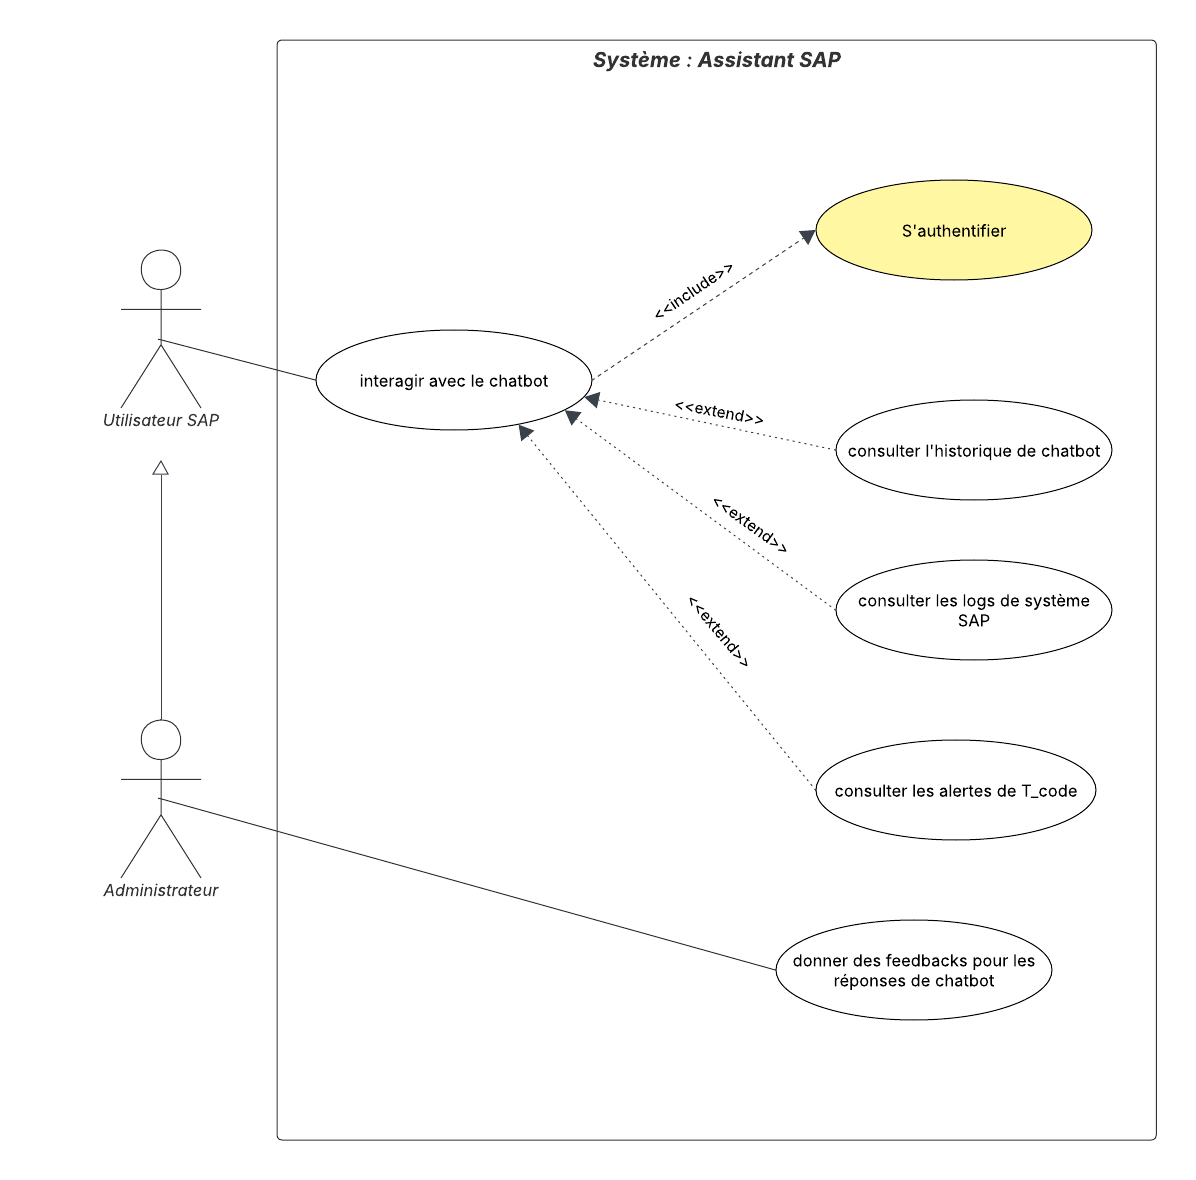
\includegraphics[width=0.9\textwidth]{images/casutilisation.png}
    \caption[Diagramme de cas d'utilisation]{Diagramme de cas d'utilisation général du système déployé}
    \label{fig:usecase_deploy}
\end{figure}

\subsection{Technologies utilisées}

L'ensemble de la pile technologique mise en œuvre est résumé dans le tableau~\ref{tab:tech_stack}.

\begin{table}[H]
\centering
\caption{Pile technologique du système déployé}
\label{tab:tech_stack}
\begin{tabularx}{\textwidth}{|l|l|X|}
\hline
\textbf{Couche} & \textbf{Technologie} & \textbf{Rôle} \\
\hline
Frontend & React 19 + SAP UI5 Web Components & Interface utilisateur, affichage du chatbot \\
\hline
Backend & SAP CAP v8 + Express.js & Services OData, proxy vers l'API RAG (port 4004) \\
\hline
Base de données & MongoDB Atlas & Stockage des données de monitoring SAP (18 collections) \\
\hline
API RAG & FastAPI + Uvicorn & Exposition du pipeline RAG en REST (port 8000) \\
\hline
LLM & Ollama (llama3.2:3b / qwen2.5:7b) & Génération locale des réponses (port 11434) \\
\hline
Embeddings & BAAI/bge-large-en-v1.5 & Vectorisation des requêtes et des documents \\
\hline
Base vectorielle & PostgreSQL + pgvector & Stockage et recherche hybride (port 5432) \\
\hline
\end{tabularx}
\end{table}


% ─────────────────────────────────────────────────────────────────────────────

% ─────────────────────────────────────────────────────────────
\section{Déploiement du système RAG}
% ─────────────────────────────────────────────────────────────

\subsection{Configuration de l'environnement}

Le système RAG est configuré à travers un fichier \texttt{.env} qui centralise les paramètres d'accès aux services externes. Les trois variables essentielles sont la chaîne de connexion à la base de données PostgreSQL, et les noms des modèles LLM disponibles via Ollama

\subsection{Infrastructure de la base de données vectorielle}

\begin{lstlisting}[language=SQL, caption={Création de l'index vectoriel HNSW sur la table sap\_chunks}]
CREATE INDEX sap_chunks_hnsw ON sap_chunks
    USING hnsw (embedding vector_cosine_ops)
    WITH (m = 16, ef_construction = 64);
\end{lstlisting}

% ─────────────────────────────────────────────────────────────
\subsection{Schéma de la base de données PostgreSQL}
\label{subsec:schema_bdd}
% ─────────────────────────────────────────────────────────────

La base de données PostgreSQL du système héberge \textbf{21 tables} organisées en quatre
groupes fonctionnels, chacun correspondant à un rôle distinct dans l'architecture RAG déployée~:

\begin{itemize}[leftmargin=2em]
  \item \textbf{Tables fondamentales RAG/CAG~:} \texttt{sap\_chunks} (76~463 vecteurs de
        dimension 1~024, index HNSW cosinus) et \texttt{qa\_cache} (cache sémantique des
        réponses générées avec leurs embeddings de requête).
  \item \textbf{Tables d'interaction utilisateur~:} \texttt{conversations} (historique de
        dialogue multi-tours avec détection d'intention et réécriture de requête) et
        \texttt{admin\_feedback} (notations et corrections humaines avec vecteur de la
        question originale pour invalidation du cache).
  \item \textbf{Tables de monitoring SAP~:} 12~tables alimentées en continu via PyRFC,
        correspondant aux T-codes de supervision~: SM37, SM51, SM66, SM12, SM13, SM58,
        SMQ1, SOST, SP01, ST03N, ST13, ST22.
  \item \textbf{Tables de métriques système~:} 5~tables de métriques OS et base de données
        (\texttt{cpu}, \texttt{memory}, \texttt{fsys}, \texttt{db02}, \texttt{mss\_db}).
\end{itemize}

La figure~\ref{fig:class_core} présente le diagramme de classes détaillé des quatre tables
fondamentales avec l'ensemble de leurs attributs et les associations logiques entre elles.
La figure~\ref{fig:class_monitoring} présente les 17~tables de monitoring et de métriques dans
un format compact.

\begin{figure}[H]
\centering
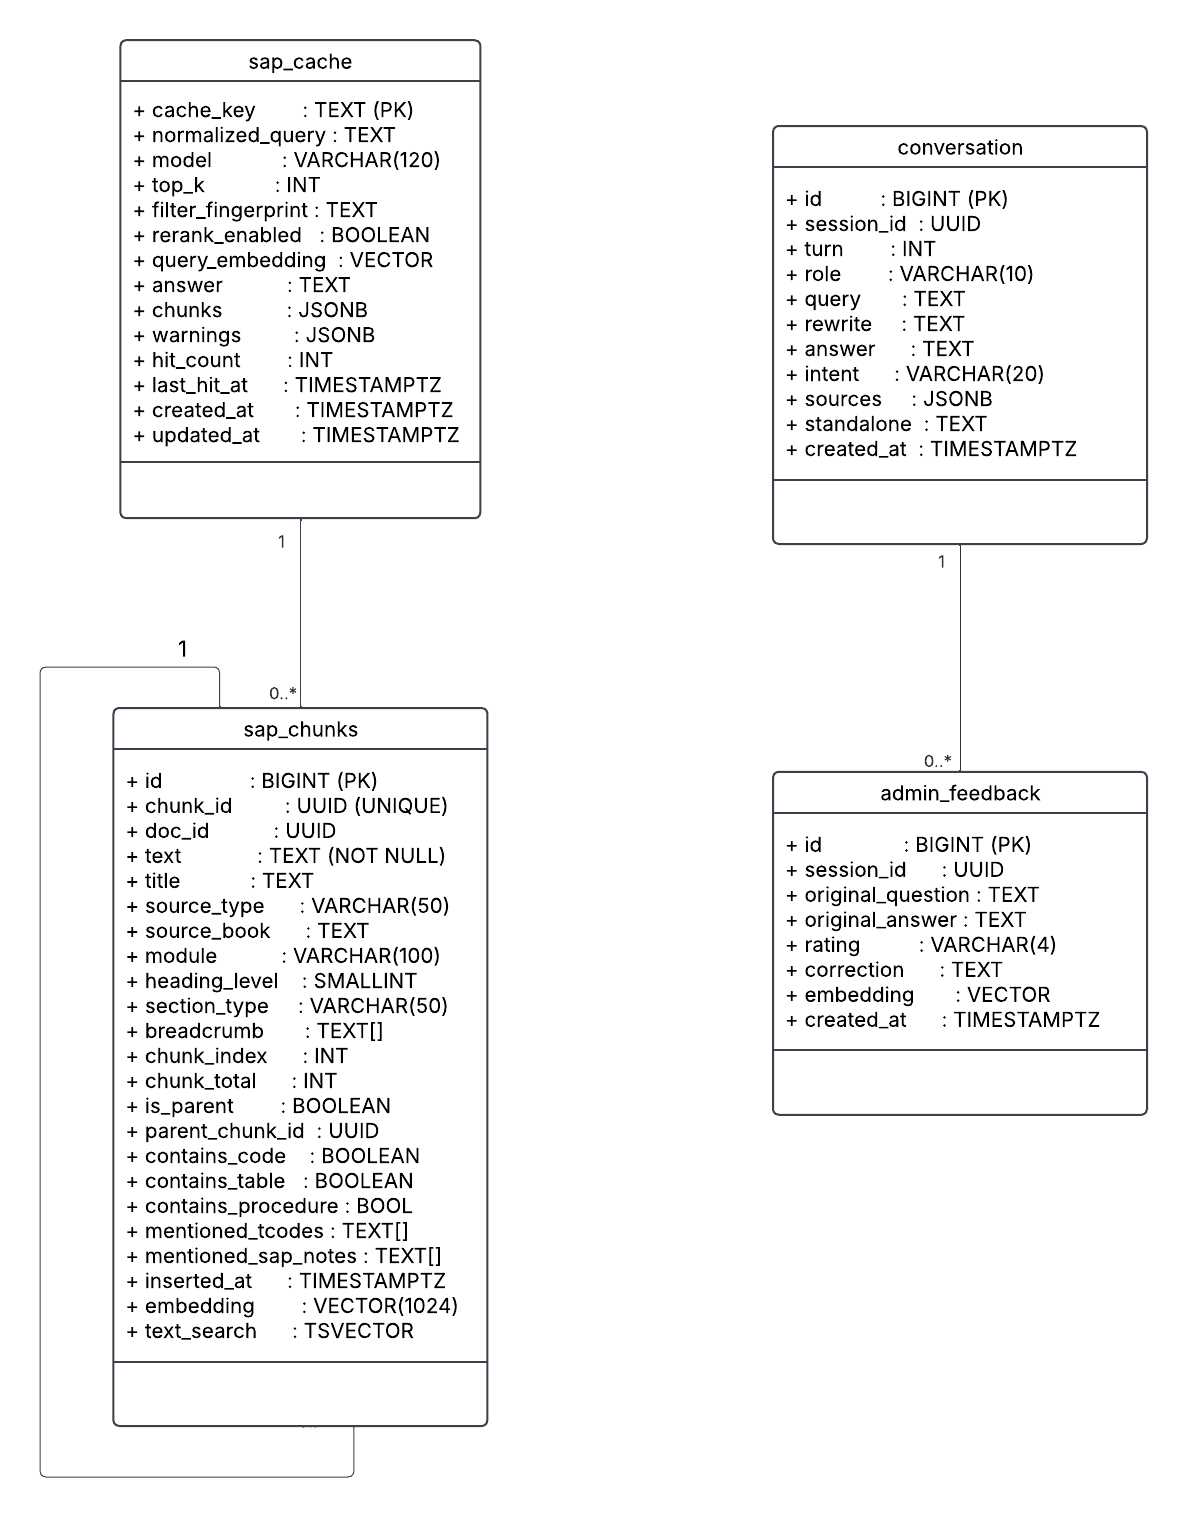
\includegraphics[width=0.90\textwidth]{images/Blank diagram.png}
\caption[Diagramme de classes (PostgreSQL)]{Diagramme de classes --- Tables fondamentales du système RAG (PostgreSQL)}
\label{fig:class_core}
\end{figure}


\subsection{Démarrage de l'API FastAPI}

Le serveur FastAPI est lancé via \textbf{Uvicorn}, le serveur ASGI de référence pour les applications Python asynchrones~:

\begin{lstlisting}[language=sh, caption={Commande de démarrage de l'API RAG}]
cd C:\Users\Youss\Documents\RAG_SAP\rag
uvicorn api:app --host 0.0.0.0 --port 8000 --reload
\end{lstlisting}

\subsection{Endpoints REST exposés}

L'API FastAPI expose trois endpoints documentés automatiquement via Swagger UI (\texttt{http://localhost:8000/docs})~:

\begin{table}[H]
\centering
\caption{Endpoints de l'API RAG (api.py)}
\label{tab:api_endpoints}
\begin{tabularx}{\textwidth}{|l|l|X|}
\hline
\textbf{Méthode} & \textbf{Endpoint} & \textbf{Description} \\
\hline
\texttt{POST} & \texttt{/query} & Reçoit une question et un session\_id, exécute le pipeline RAG, renvoie la réponse avec sources et avertissements \\
\hline
\texttt{DELETE} & \texttt{/session/\{session\_id\}} & Supprime l'historique de conversation associé à une session \\
\hline
\texttt{GET} & \texttt{/health} & Vérifie la disponibilité du service et retourne le modèle actif \\
\hline
\end{tabularx}
\end{table}

Le corps de la requête \texttt{POST /query} accepte les paramètres suivants~:

\begin{lstlisting}[language=Python, caption={Schéma de la requête POST /query (api.py)}]
class QueryRequest(BaseModel):
    question:      str
    session_id:    str = ""
    top_k:         int = TOP_K          # defaut : 5
    model:         str = OLLAMA_MODEL   # defaut : llama3.2:3b
    filter_tcode:  Optional[str] = None
    filter_module: Optional[str] = None
    filter_source: Optional[str] = None
\end{lstlisting}

\begin{figure}[H]
\centering
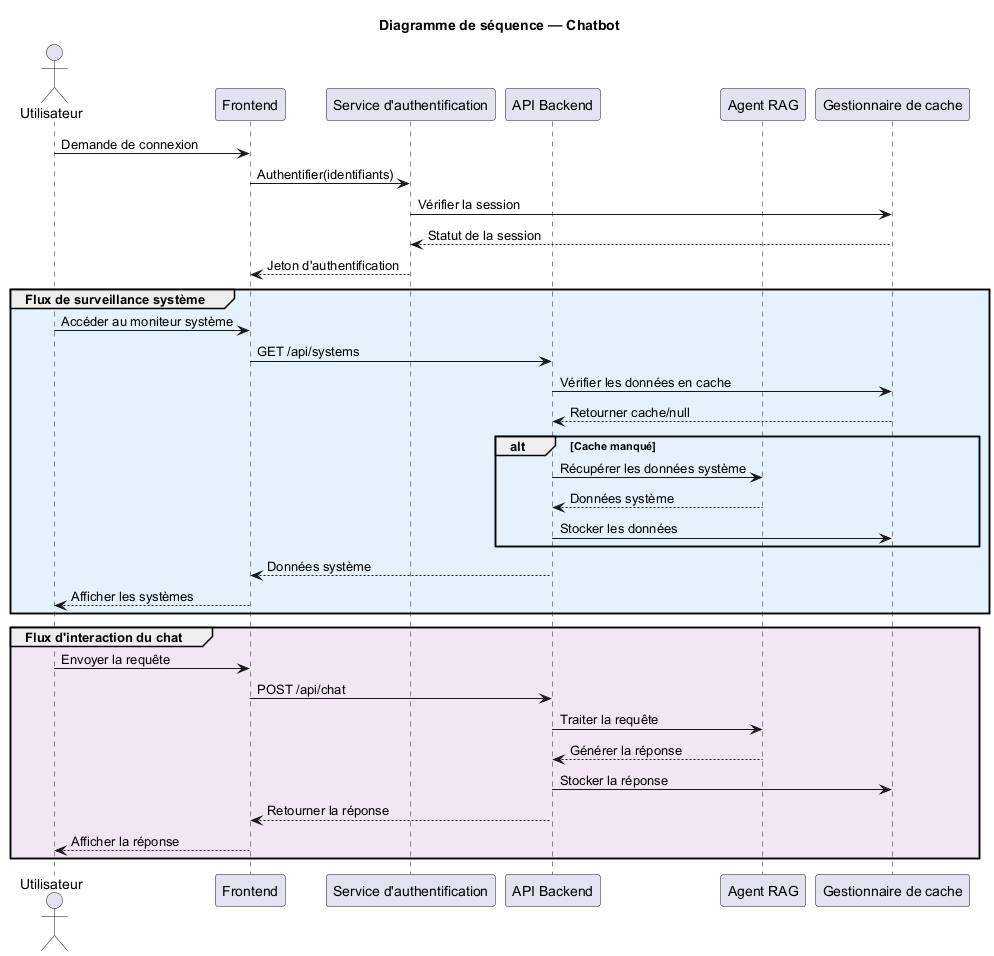
\includegraphics[width=\textwidth]{images/sequence_chatbot_fr.png}
\caption[Diagramme de séquence — interaction complète]{Diagramme de séquence  cycles complets d'interaction~: initialisation de session, surveillance SAP et chatbot RAG}
\label{fig:sequence_requete}
\end{figure}

\subsection{Paramètres clés du pipeline}

Le tableau~\ref{tab:pipeline_params} regroupe les hyperparamètres déterminants du pipeline RAG déployé en production~:

\begin{table}[H]
\centering
\caption{Paramètres de configuration du pipeline RAG (rag\_pipeline.py)}
\label{tab:pipeline_params}
\begin{tabularx}{\textwidth}{|l|l|X|}
\hline
\textbf{Paramètre} & \textbf{Valeur} & \textbf{Rôle} \\
\hline
\texttt{FETCH\_K} & 15 & Nombre de candidats récupérés par recherche vectorielle \\
\hline
\texttt{RERANK\_K} & 10 & Nombre de candidats transmis au cross-encoder après RRF \\
\hline
\texttt{TOP\_K} & 5 & Nombre final de chunks injectés dans le prompt LLM \\
\hline
\texttt{CAG\_MAX\_CHUNKS} & 3 & Chunks pré-chargés max pour les requêtes T-code (CAG) \\
\hline
\texttt{MIN\_SCORE} & 0.05 / 0.30 & Seuil minimal de similarité cosinus (adaptatif selon l'intention) \\
\hline
\texttt{MIN\_RERANK\_SCORE} & 2.0 & Seuil de rejet par le cross-encoder (échelle $-10$ à $+10$) \\
\hline
\texttt{MAX\_CHUNKS\_PER\_SOURCE} & 3 & Déduplication : maximum de chunks par source \\
\hline
$W_{\text{vec}}$ / $W_{\text{BM25}}$ & 0.4 / 0.6 & Poids de fusion RRF (BM25 privilégié pour corpus SAP) \\
\hline
\texttt{NUM\_CTX} & 4~096 & Fenêtre de contexte du LLM Ollama (en tokens) \\
\hline
\texttt{Temperature} & 0.1 & Température de génération (réponses déterministes) \\
\hline
\end{tabularx}
\end{table}

% ─────────────────────────────────────────────────────────────
\section{Intégration du chatbot dans l'application web}
% ─────────────────────────────────────────────────────────────

\subsection{Vue d'ensemble de l'intégration}

L'intégration du chatbot dans AutoMoni a été réalisée selon une architecture en trois niveaux~: la \textbf{définition du service} en CDS (Core Data Services), l'\textbf{implémentation du handler} en JavaScript côté CAP, et les \textbf{composants React} côté frontend.

% ── PLACEHOLDER 3 ────────────────────────────────────────────────────────────
% Diagramme à réaliser : architecture des composants de l'intégration chatbot
% Composants : ChatPanel.jsx, AppShell.jsx, chat-service.cds, chat-service.js, api.py
% Suggestions : diagramme de composants UML ou schéma bloc en draw.io

% ─────────────────────────────────────────────────────────────────────────────

\subsection{Définition du service OData (CAP CDS)}

Le service de chatbot est défini dans le fichier \texttt{chat-service.cds} à l'aide du langage CDS de SAP. Il expose une action OData qui accepte la question de l'utilisateur et un identifiant de session, et retourne la réponse structurée du système RAG~:

\begin{lstlisting}[language=SQL, caption={Définition du service chatbot en CDS (chat-service.cds)}]
service ChatService {
  action query(question: String, session_id: String) returns {
    answer:     String;
    sources:    array of String;
    warnings:   array of String;
    session_id: String;
  };
}
\end{lstlisting}

Cette définition génère automatiquement l'endpoint OData \texttt{POST /odata/v4/chat/query}, documenté et typé, directement accessible depuis le frontend React.



\subsection{Composants React du chatbot}

Le chatbot est implémenté côté frontend sous deux formes complémentaires~:

\begin{itemize}[leftmargin=2em]
  \item \textbf{Page dédiée} (\texttt{/chatbot})~: le composant \texttt{Chatbot.jsx} (515 lignes) offre une interface complète avec historique de conversations organisées en sessions, liste des conversations précédentes, zone de réponse avec rendu Markdown via \texttt{react-markdown}, et boutons d'action (nouvelle conversation, effacement).

  \item \textbf{ChatPanel — Tiroir latéral}~: exporté depuis \texttt{Chatbot.jsx}, ce panneau coulissant est intégré dans le composant \texttt{AppShell.jsx} et rendu accessible depuis toutes les pages de l'application via le bouton IA dans la \texttt{ShellBar}. Il est monté paresseusement (\textit{lazy mount}) à la première ouverture afin d'éviter un flash CSS indésirable~:

\begin{lstlisting}[language=JavaScript, caption={Montage paresseux du ChatPanel dans AppShell.jsx}]
const [isChatOpen,    setIsChatOpen]    = useState(false)
const [chatHasOpened, setChatHasOpened] = useState(false)

const onChatbotClick = () => {
  if (!chatHasOpened) setChatHasOpened(true)
  setIsChatOpen(prev => !prev)
}

{chatHasOpened && (
  <ChatPanel open={isChatOpen} onClose={() => setIsChatOpen(false)} />
)}
\end{lstlisting}
\end{itemize}

\subsection{Chatbot et évaluation intégrée en temps réel}
\label{subsec:chatbot-eval}

L'intégration du pipeline d'évaluation directement dans la boucle de traitement du chatbot constitue un apport majeur par rapport à une évaluation \textit{offline} classique. Plutôt que d'utiliser un juge LLM coûteux à chaque appel (comme G-Eval), le système repose sur deux mécanismes complémentaires déclenchés automatiquement à chaque réponse~:

\begin{enumerate}[leftmargin=2em]
  \item \textbf{Détection déterministe des hallucinations}~: la fonction \texttt{check\_hallucinations()} analyse la réponse générée à la recherche de T-codes SAP et de numéros de notes SAP qui ne figurent pas dans les chunks récupérés. Toute mention identifiée comme non ancrée dans les sources est supprimée par \texttt{sanitize\_answer()} avant renvoi à l'utilisateur. Ce mécanisme s'exécute en moins d'une milliseconde sans appel LLM supplémentaire.

  \item \textbf{Attribution des sources}~: les chunks utilisés pour construire la réponse sont retournés dans le champ \texttt{sources} de la réponse JSON, sous forme de références structurées (\textit{«~titre du livre $>$ section~»}).
\end{enumerate}

Ces deux informations sont remontées dans l'interface utilisateur via le contrat d'API défini dans \texttt{chat-service.cds}~:

\begin{lstlisting}[language=SQL, caption={Champs d'évaluation retournés par le service RAG}]
returns {
  answer:   String;          -- reponse nettoyee
  sources:  array of String; -- references des chunks utilises
  warnings: array of String; -- hallucinations detectees et supprimees
  session_id: String;
}
\end{lstlisting}

Le composant React \texttt{BotMessageContent} interprète ces champs et affiche, sous chaque réponse du bot, un indicateur de qualité et la liste des sources consultées~:

\begin{itemize}[leftmargin=2em]
  \item \textbf{Badge vert «~\checkmark~Réponse vérifiée~»}~: aucun avertissement détecté, la réponse est intégralement ancrée dans les sources récupérées.
  \item \textbf{Badge orange «~$\triangle$~N avertissement(s)~»}~: au moins une affirmation a été filtrée pour risque d'hallucination, l'utilisateur est averti.
  \item \textbf{Section «~Sources~» dépliable}~: liste des références documentaires utilisées, permettant à l'utilisateur de vérifier l'origine de chaque information.
\end{itemize}

\begin{lstlisting}[language=JavaScript, caption={Rendu du badge qualité et des sources dans BotMessageContent (Chatbot.jsx)}]
const BotMessageContent = ({ message }) => (
  <>
    <Markdown>{message.text}</Markdown>
    {(message.sources?.length > 0 || message.warnings?.length > 0) && (
      <div className="ag-eval-footer">
        <span className={`ag-quality-badge ${
          message.warnings?.length > 0
            ? 'ag-quality-badge--warn'
            : 'ag-quality-badge--ok'
        }`}>
          {message.warnings?.length > 0
            ? `Warning: ${message.warnings.length} hallucination(s) filtered`
            : 'Response verified'}
        </span>
        <details className="ag-sources">
          <summary>{message.sources.length} source(s)</summary>
          <ul>{message.sources.map((src, i) => <li key={i}>{src}</li>)}</ul>
        </details>
      </div>
    )}
  </>
)
\end{lstlisting}

Cette approche est délibérément \textbf{déterministe et légère}~: contrairement à RAGAS ou G-Eval qui nécessitent un second appel LLM pour scorer la réponse, la détection par règles (T-codes, numéros de notes) est instantanée et 100\,\% reproductible. Elle constitue un mécanisme de premier niveau suffisant pour alerter l'utilisateur sur les cas les plus risqués, RAGAS étant réservé à l'évaluation \textit{offline} en batch du pipeline.

\subsection{Intelligence de navigation — T-codes vers pages monitoring}

Une fonctionnalité avancée du chatbot est sa capacité à détecter dans le message de l'utilisateur une \textbf{intention de navigation} vers une page de monitoring, et à y rediriger automatiquement. Le composant \texttt{Chatbot.jsx} embarque un dictionnaire de 18 T-codes SAP mappés à leurs routes React~:

\begin{lstlisting}[language=JavaScript, caption={Mapping T-codes vers routes de navigation (Chatbot.jsx)}]
const TCODE_ROUTES = {
  st22:  { path: '/st22',  label: 'Runtime Errors (ST22)'    },
  sm37:  { path: '/sm37',  label: 'Background Jobs (SM37)'   },
  sm13:  { path: '/sm13',  label: 'Update Records (SM13)'    },
  sm66:  { path: '/sm66',  label: 'Work Processes (SM66)'    },
  db02:  { path: '/db02',  label: 'Database Space (DB02)'    },
  sm58:  { path: '/sm58',  label: 'RFC Monitoring (SM58)'    },
  smq1:  { path: '/smq1',  label: 'Outbound Queue (SMQ1)'   },
  // ... 11 autres T-codes
}
\end{lstlisting}

Lorsque l'utilisateur formule un message contenant à la fois un T-code reconnu et un mot-clé d'intention de navigation (\texttt{open}, \texttt{go to}, \texttt{ouvre}, \texttt{affiche}, etc.), le chatbot effectue une redirection directe vers la page correspondante, sans interroger l'API RAG. Cette détection supporte également l'extraction du \textbf{SID} (System ID, ex. \texttt{PRD}, \texttt{P01}) et d'un \textbf{filtre de date} depuis le message naturel.

% ─────────────────────────────────────────────────────────────
\section{Interface utilisateur — Présentation}
% ─────────────────────────────────────────────────────────────

\subsection{Page chatbot dédiée}

La page chatbot, accessible via la route \texttt{/chatbot}, propose une interface structurée en deux panneaux~: à gauche, la liste des conversations historiques identifiées par un titre auto-généré, et à droite, la conversation active avec l'assistant. Parmi ses fonctionnalités principales~:

\begin{itemize}[leftmargin=2em]
  \item \textbf{Gestion des sessions}~: chaque conversation est identifiée par un UUID de session unique, qui est transmis à l'API RAG afin de maintenir le contexte conversationnel côté serveur.
  \item \textbf{Quick Prompts}~: trois suggestions de questions fréquentes (\textit{Show top runtime errors today}, \textit{Any failed background jobs right now?}, \textit{Summarize DB space alerts}) sont proposées à l'utilisateur pour faciliter la prise en main.
  \item \textbf{Indicateur de traitement}~: un \textit{BusyIndicator} SAP UI5 s'affiche pendant le temps de réponse du système.
  \item \textbf{Avertissements d'hallucinations}~: si l'API RAG détecte un T-code ou une note SAP potentiellement hallucin\'{e}(e), un avertissement est affiché sous la réponse.
\end{itemize}

\subsection{ChatPanel : Tiroir latéral universel}

Le composant \texttt{ChatPanel} est directement intégré au sein du shell applicatif \texttt{AppShell.jsx}. Il peut être ouvert depuis n’importe quelle page de l’application grâce au bouton IA (\textit{icône d’intelligence artificielle}) positionné dans la \texttt{ShellBar}, en haut à droite de l’interface. Lors de son activation, le panneau apparaît latéralement depuis la droite via une animation de type \textit{slide-in}, offrant à l’utilisateur la possibilité d’interagir avec l’assistant conversationnel tout en conservant le contexte de la page de monitoring actuellement affichée.
% Placeholder pour captures d'écran
\begin{figure}[H]
\centering
 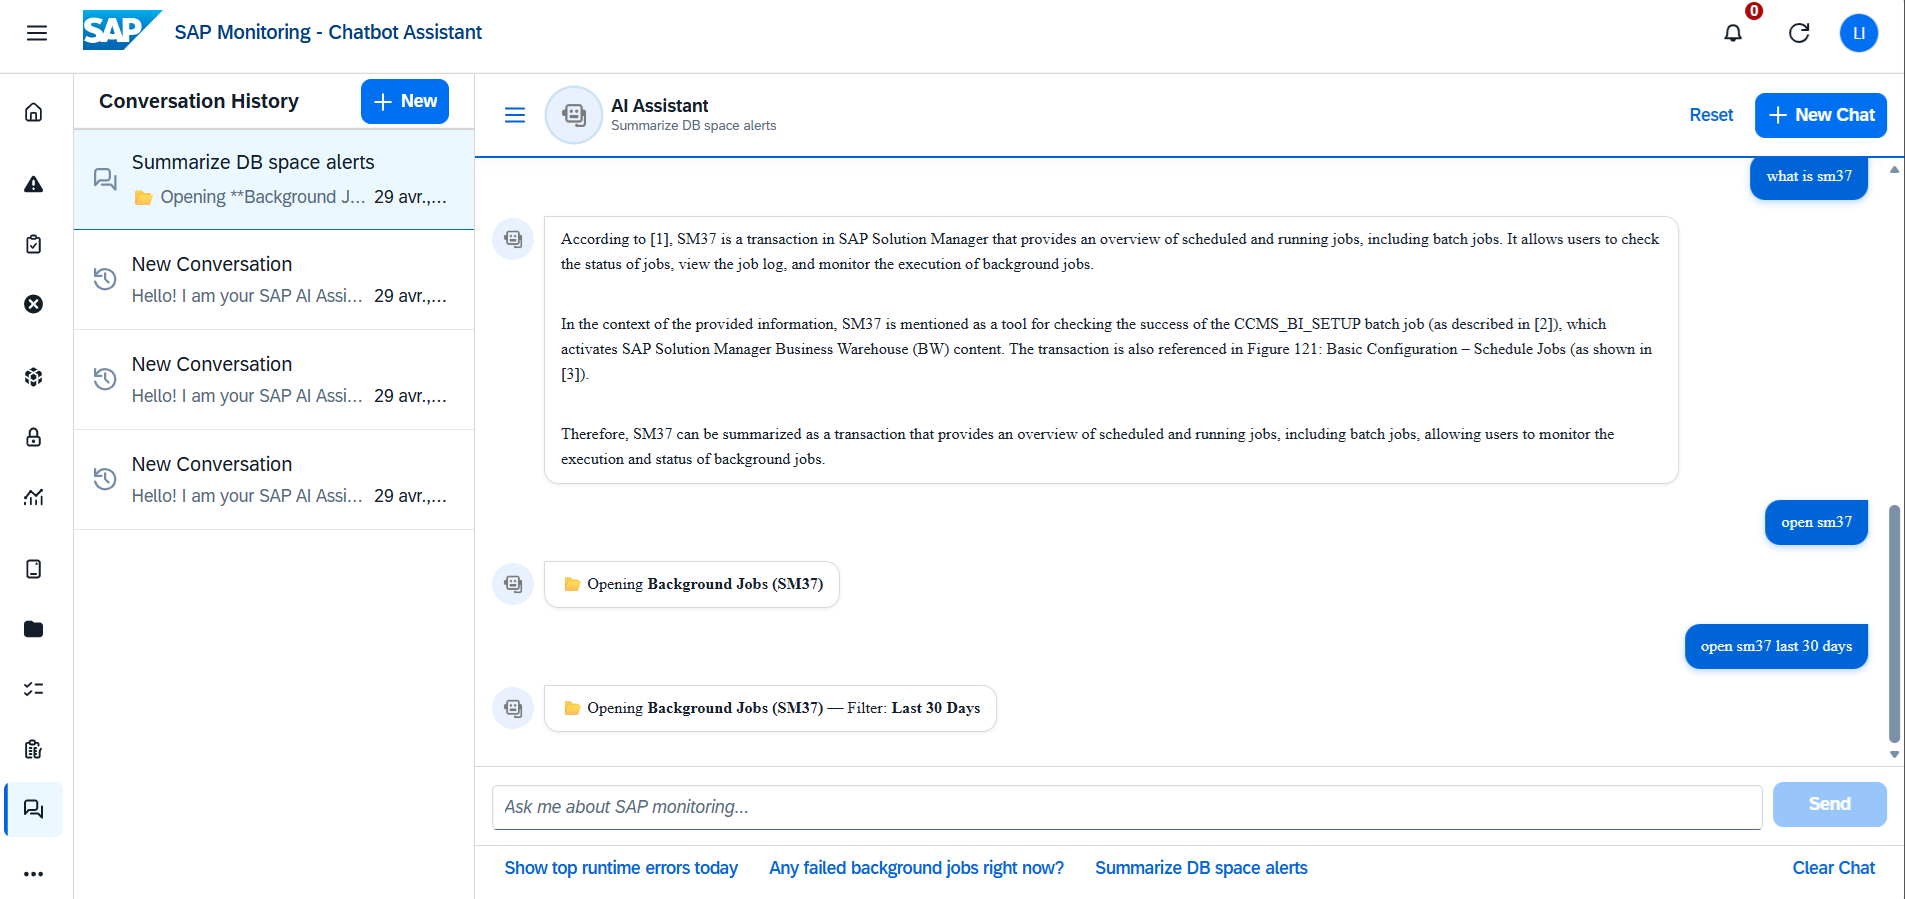
\includegraphics[width=0.9\textwidth]{images/chat.png}
\caption[Interface chatbot avec historique]{Interface de la page chatbot dédiée avec historique de conversations}
\label{fig:chatbot_page}
\end{figure}

\begin{figure}[H]
\centering
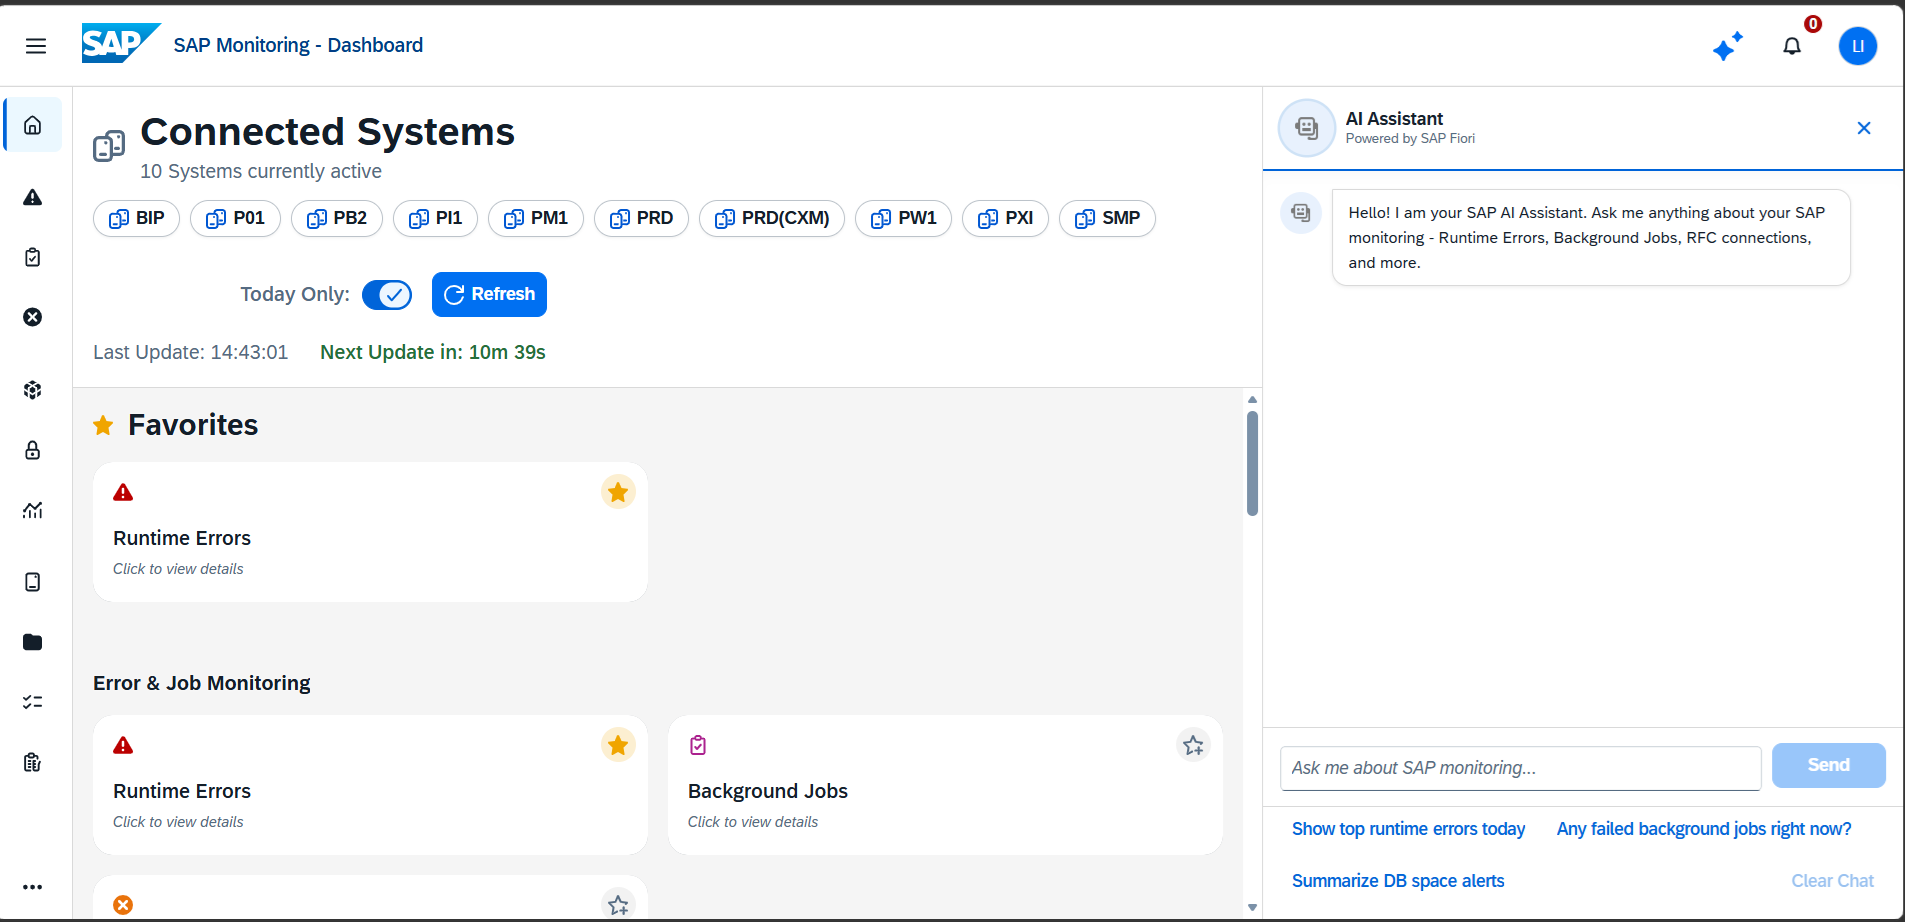
\includegraphics[width=0.9\textwidth]{images/lateral.png}
\caption[ChatPanel en tiroir latéral]{ChatPanel intégré en tiroir latéral sur une page de monitoring SAP}
\label{fig:chatpanel}
\end{figure}

% ─────────────────────────────────────────────────────────────
\section{Sélection du modèle LLM et benchmarking}
% ─────────────────────────────────────────────────────────────

\subsection{Protocole d'évaluation}

Afin de comparer objectivement les deux configurations LLM disponibles, un benchmark automatisé a été conduit le 12 mai 2026. Il porte sur un ensemble de \textbf{10 questions représentatives} des cas d'usage réels du système, couvrant des T-codes BASIS courants~:

\begin{enumerate}[leftmargin=2em]
  \item How to monitor background jobs in SM37?
  \item How to analyze a short dump in ST22?
  \item How to configure transport routes in STMS?
  \item How to manage user roles with SU01 and PFCG?
  \item How to create an ABAP program using SE38?
  \item What is a BAPI and how to test it with SE37?
  \item How to reprocess IDoc errors using BD87?
  \item How to analyze authorization errors with SU53?
  \item How to read system logs in SM21?
  \item How to analyze work processes with SM50?
\end{enumerate}

Les deux modèles évalués sont \textbf{LLaMA~3.2:3b} (modèle rapide, 3 milliards de paramètres) et \textbf{Qwen~2.5:7b} (modèle de qualité supérieure, 7 milliards de paramètres). Les métriques calculées sont le \textbf{Recall@K} (proportion de questions ayant au moins un chunk pertinent dans les K premiers résultats), le \textbf{MRR} (\textit{Mean Reciprocal Rank}, position moyenne du premier chunk pertinent) et le \textbf{nDCG} (\textit{Normalized Discounted Cumulative Gain}, qualité globale du classement). Les valeurs de K testées sont $K \in \{1, 3, 5, 10, 12\}$.

\subsection{Résultats}

La figure~\ref{fig:benchmark} présente les résultats visuels du benchmark comparatif entre les deux configurations LLM sur l'ensemble des métriques de retrieval.

\begin{figure}[H]
\centering
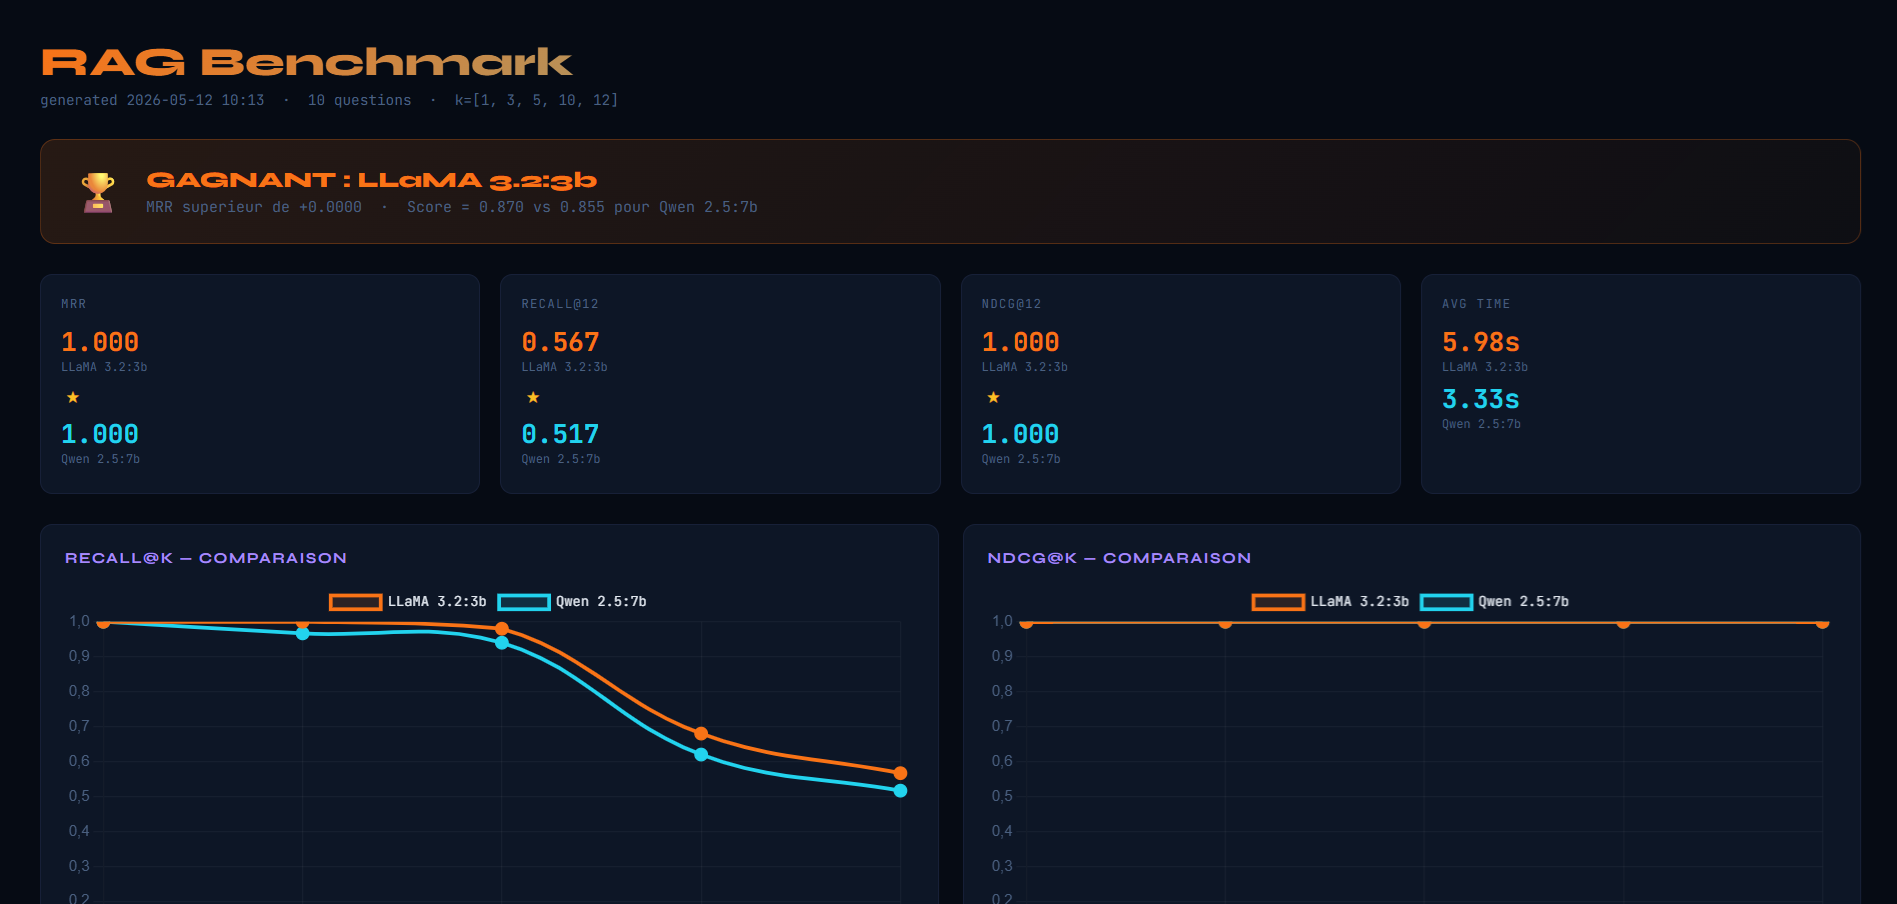
\includegraphics[width=0.95\textwidth]{images/bench.png}
\caption[Benchmark RAG — LLaMA 3.2:3b vs Qwen 2.5:7b]{Résultats du benchmark RAG — LLaMA 3.2:3b vs Qwen 2.5:7b (12 mai 2026, 76~463 vecteurs)}
\label{fig:benchmark}
\end{figure}

\subsection{Analyse des résultats}

Les résultats du benchmark mettent en évidence plusieurs constats~:

\begin{itemize}[leftmargin=2em]
  \item \textbf{Recall@K croissant}~: le rappel augmente logiquement avec K pour les deux modèles, atteignant des valeurs élevées à K=10 et K=12, confirmant que la base documentaire contient les informations nécessaires pour répondre aux questions posées.

  \item \textbf{Qualité de classement}~: le nDCG reflète la capacité du pipeline à placer les chunks les plus pertinents en tête de liste. La fusion RRF avec pondération asymétrique (BM25~: 0.6, vectoriel~: 0.4) favorise la précision lexicale, essentielle pour les T-codes SAP.

  \item \textbf{Impact des paramètres}~: Qwen~2.5:7b utilise un seuil de reranking (\texttt{MIN\_RERANK\_SCORE~=~2.0}) et un \texttt{FETCH\_K~=~40} plus élevés que LLaMA~3.2:3b (\texttt{MIN\_RERANK\_SCORE~=~1.0}, \texttt{FETCH\_K~=~30}), ce qui explique une sélectivité différente dans les résultats.

  \item \textbf{Compromis vitesse/qualité}~: LLaMA~3.2:3b offre des temps de réponse significativement plus courts, tandis que Qwen~2.5:7b produit des réponses de meilleure qualité rédactionnelle. Le choix du modèle peut être configuré dynamiquement via la variable \texttt{model} de la requête API.
\end{itemize}

% ─────────────────────────────────────────────────────────────
\section{Limites et perspectives}
% ─────────────────────────────────────────────────────────────

\subsection{Limites du déploiement actuel}

Malgré les performances satisfaisantes observées lors du benchmark, plusieurs limitations du déploiement actuel méritent d'être soulignées~:

\begin{itemize}[leftmargin=2em]
  \item \textbf{CORS ouvert en développement}~: La politique CORS de l'API FastAPI est actuellement configurée en mode permissif (\texttt{allow\_origins=["*"]}), adapté à un environnement de développement. Une configuration restrictive sera nécessaire pour un déploiement en production.

  \item \textbf{Cache sémantique en mémoire}~: Le cache sémantique du pipeline RAG est stocké uniquement en mémoire vive du processus. Son contenu est perdu à chaque redémarrage et ne peut pas être partagé entre plusieurs instances, ce qui limite son efficacité dans une architecture distribuée.

  \item \textbf{LLM local limité}~: Le modèle \texttt{llama3.2:3b} déployé localement via Ollama, bien qu'adapté à un contexte \textit{on-premise}, reste moins performant que les grands modèles hébergés dans le cloud (GPT-4o, Claude Sonnet) sur des questions complexes nécessitant un raisonnement approfondi.

  \item \textbf{Gestion des sessions en mémoire}~: Les sessions de conversation de l'API FastAPI sont stockées dans un dictionnaire Python en mémoire. En cas de redémarrage du service, toutes les sessions actives sont perdues. La persistance des sessions dans la base de données PostgreSQL est déjà implémentée mais dépend d'un mécanisme asynchrone de sauvegarde.

  \item \textbf{Détection d'hallucinations par heuristiques}~: La validation anti-hallucination repose sur des expressions régulières pour les T-codes et les numéros de notes SAP. Les affirmations factuellement erronées ne contenant pas d'identifiants SAP explicites ne sont pas détectées.
\end{itemize}

\subsection{Perspectives d'amélioration}

Plusieurs axes d'amélioration peuvent être envisagés pour renforcer le système à court et moyen terme~:

\begin{itemize}[leftmargin=2em]
  \item \textbf{Déploiement Cloud Foundry}~: Les fichiers \texttt{mta.yaml} et \texttt{manifest.yml} sont déjà configurés pour un déploiement sur SAP BTP (\textit{Business Technology Platform}) via Cloud Foundry. Cette étape permettrait de bénéficier d'une haute disponibilité, d'un équilibrage de charge et d'une authentification XSUAA intégrée.

  \item \textbf{Cache sémantique distribué}~: L'intégration d'un cache Redis permettrait de partager le cache sémantique entre plusieurs instances de l'API RAG et de le persister entre les redémarrages.

  \item \textbf{Modèle LLM plus performant}~: L'intégration d'un modèle de grande taille (qwen2.5:7b déjà supporté, ou un modèle cloud via API) améliorerait la qualité des réponses sur les requêtes complexes.

  \item \textbf{Mise à jour incrémentale de la base de connaissances}~: Un pipeline de synchronisation incrémentale (déjà prototypé dans \texttt{conv\_databaseMONGODB/}) permettrait d'enrichir automatiquement la base documentaire à mesure que de nouvelles notes SAP ou documentations sont publiées.

  \item \textbf{Collecte de feedback utilisateur}~: L'ajout d'un mécanisme de notation des réponses (pouce haut/pouce bas) permettrait de constituer un jeu de données d'évaluation continue et d'identifier les points faibles du système en production réelle.
\end{itemize}

% ─────────────────────────────────────────────────────────────
\section*{Conclusion}
% ─────────────────────────────────────────────────────────────
Ce chapitre a présenté le déploiement complet du système RAG SAP dans le cadre de la méthodologie CRISP-DM. L’architecture développée repose sur trois couches complémentaires : un backend Python/FastAPI pour le moteur RAG, un service SAP CAP assurant l’exposition OData, et une interface React SAP UI5 intégrant le chatbot. Les résultats du benchmark ont confirmé l’efficacité du pipeline hybride de retrieval sur un corpus SAP volumineux de 76~463 vecteurs. En environnement de production, la solution permet aux administrateurs SAP BASIS d’obtenir rapidement des réponses techniques fiables directement depuis l’interface de monitoring. Enfin, les perspectives d’évolution, notamment l’intégration sur SAP BTP et l’utilisation de modèles LLM plus performants, ouvrent la voie à une industrialisation avancée de la plateforme.
% ---- Bibliographie ----
\bibliographystyle{plainnat}
\bibliography{references}
\end{document}